


% ******************************* PhD Thesis Template **************************
% Please have a look at the README.md file for info on how to use the template

% \documentclass[a4paper,12pt,oneside,customfont,numbered,print]{Classes/PhDThesisPSnPDF}
\documentclass[a4paper,11pt,oneside,customfont,numbered]{Classes/PhDThesisPSnPDF}
% \documentclass[a4paper,11pt,oneside,customfont,numbered,print]{Classes/PhDThesisPSnPDF}
% \documentclass[a4paper,11pt,oneside,customfont,numbered,chapter]{Classes/PhDThesisPSnPDF}
% \documentclass[a4paper,11pt,oneside,customfont,numbered,chapter,draft]{Classes/PhDThesisPSnPDF}
\usepackage{indentfirst}

% ***************************** Chapter Mode ***********************************
% The chapter mode allows user to only print particular chapters with references
% Title, Contents, Frontmatter are disabled by default
% Useful option to review a particular chapter or to send it to supervisior.
% To use choose `chapter' option in the document class

\ifdefineChapter
 \includeonly{Chapter2/chapter2}
\fi

\setlength\parindent{11pt}

% Load basic packages
\usepackage{balance}       % to better equalize the last page
\usepackage{graphics}      % for EPS, load graphicx instead 
\usepackage[T1]{fontenc}   % for umlauts and other diaeresis
\usepackage{txfonts}
\usepackage{mathptmx}
% \usepackage[pdflang={en-US},pdftex]{hyperref}
\usepackage{color}
\usepackage{booktabs}
\usepackage{textcomp}
\usepackage{here}
\usepackage{multirow}
\usepackage{colortbl}
\usepackage{url}
\usepackage{subcaption}
\usepackage{subfig}

% my package
\usepackage{caption}
\usepackage{amsmath,bm}
\usepackage{here}
% \usepackage{tabularx}
% \setlength{\extrarowheight}{3pt}
% \usepackage{tabularx}
% \usepackage{arydshln}
\usepackage{colortbl,xcolor}
% \usepackage{mathspec}
% \usepackage[italic,noendash]{mathastext}
% \usepackage{amssymb}
\usepackage{makecell}
\usepackage{listings}
\usepackage{lipsum}
\usepackage{courier}

\lstset{basicstyle=\footnotesize\ttfamily,breaklines=true}
\lstset{framextopmargin=50pt,frame=bottomline}

\captionsetup[figure]{format=hang, labelformat=simple, labelsep=colon, font=small}
\captionsetup[table]{format=hang, labelformat=simple, labelsep=colon, font=small}

% ******************************************************************************
% ******************************* Class Options ********************************
% *********************** See README for more details **************************
% ******************************************************************************

% `a4paper'(The University of Cambridge PhD thesis guidelines recommends a page
% size a4 - default option) or `a5paper': A5 Paper size is also allowed as per
% the Cambridge University Engineering Deparment guidelines for PhD thesis
%
% `11pt' or `12pt'(default): Font Size 10pt is NOT recommended by the University
% guidelines
%
% `oneside' or `twoside'(default): Printing double side (twoside) or single
% side.
%
% `print': Use `print' for print version with appropriate margins and page
% layout. Leaving the options field blank will activate Online version.
%
% `index': For index at the end of the thesis
%
% `draftclassic': For draft mode without loading any images (same as draft in book)
%
% `draft': Special draft mode with line numbers, images, and water mark with
% timestamp and custom text. Position of the text can also be modified.
%
% `abstract': To generate only the title page and abstract page with
% dissertation title and name, to submit to the Student Registry
%
% `chapter`: This option enables only the specified chapter and it's references
%  Useful for review and corrections.
%
% ************************* Custom Page Margins ********************************
%
% `custommargin`: Use `custommargin' in options to activate custom page margins,
% which can be defined in the preamble.tex. Custom margin will override
% print/online margin setup.
%
% *********************** Choosing the Fonts in Class Options ******************
%
% `times' : Times font with math support. (The Cambridge University guidelines
% recommend using times)
%
% `fourier': Utopia Font with Fourier Math font (Font has to be installed)
%            It's a free font.
%
% `customfont': Use `customfont' option in the document class and load the
% package in the preamble.tex
%
% default or leave empty: `Latin Modern' font will be loaded.
%
% ********************** Choosing the Bibliography style ***********************
%
% `authoryear': For author-year citation eg., Krishna (2013)
%
% `numbered': (Default Option) For numbered and sorted citation e.g., [1,5,2]
%
% `custombib': Define your own bibliography style in the `preamble.tex' file.
%              `\RequirePackage[square, sort, numbers, authoryear]{natbib}'.
%              This can be also used to load biblatex instead of natbib
%              (See Preamble)
%
% **************************** Choosing the Page Style *************************
%
% `default (leave empty)': For Page Numbers in Header (Left Even, Right Odd) and
% Chapter Name in Header (Right Even) and Section Name (Left Odd). Blank Footer.
%
% `PageStyleI': Chapter Name next & Page Number on Even Side (Left Even).
% Section Name & Page Number in Header on Odd Side (Right Odd). Footer is empty.
%
% `PageStyleII': Chapter Name on Even Side (Left Even) in Header. Section Number
% and Section Name in Header on Odd Side (Right Odd). Page numbering in footer

% Uncomment to change page style
%\pagestyle{PageStyleII}

% ********************************** Preamble **********************************
% Preamble: Contains packages and user-defined commands and settings
% ******************************************************************************
% ****************************** Custom Margin *********************************

% Add `custommargin' in the document class options to use this section
% Set {innerside margin / outerside margin / topmargin / bottom margin}  and
% other page dimensions
\ifsetCustomMargin
  \RequirePackage[left=37mm,right=30mm,top=35mm,bottom=30mm]{geometry}
  \setFancyHdr % To apply fancy header after geometry package is loaded
\fi

% Add spaces between paragraphs
%\setlength{\parskip}{0.5em}
% Ragged bottom avoids extra whitespaces between paragraphs
\raggedbottom
% To remove the excess top spacing for enumeration, list and description
%\usepackage{enumitem}
%\setlist[enumerate,itemize,description]{topsep=0em}

% *****************************************************************************
% ******************* Fonts (like different typewriter fonts etc.)*************

% Add `customfont' in the document class option to use this section

\ifsetCustomFont
  % Set your custom font here and use `customfont' in options. Leave empty to
  % load computer modern font (default LaTeX font).
  %\RequirePackage{helvet}
  
  % Suigin Added for Japanese Font
  \RequirePackage{zxjatype}
  \RequirePackage[ipa]{zxjafont}

  % For use with XeLaTeX
  %  \setmainfont[
  %    Path              = ./libertine/opentype/,
  %    Extension         = .otf,
  %    UprightFont = LinLibertine_R,
  %    BoldFont = LinLibertine_RZ, % Linux Libertine O Regular Semibold
  %    ItalicFont = LinLibertine_RI,
  %    BoldItalicFont = LinLibertine_RZI, % Linux Libertine O Regular Semibold Italic
  %  ]
  %  {libertine}
  %  % load font from system font
  %  \newfontfamily\libertinesystemfont{Linux Libertine O}
\fi

% *****************************************************************************
% **************************** Custom Packages ********************************

% ************************* Algorithms and Pseudocode **************************

%\usepackage{algpseudocode}


% ********************Captions and Hyperreferencing / URL **********************

% Captions: This makes captions of figures use a boldfaced small font.
%\RequirePackage[small,bf]{caption}

\RequirePackage[labelsep=space,tableposition=top]{caption}
\renewcommand{\figurename}{Fig.} %to support older versions of captions.sty


% *************************** Graphics and figures *****************************

%\usepackage{rotating}
%\usepackage{wrapfig}

% Uncomment the following two lines to force Latex to place the figure.
% Use [H] when including graphics. Note 'H' instead of 'h'
\usepackage{here}
%\usepackage{float}
%\restylefloat{figure}

% Subcaption package is also available in the sty folder you can use that by
% uncommenting the following line
% This is for people stuck with older versions of texlive
%\usepackage{sty/caption/subcaption}
\usepackage{subcaption}

% ********************************** Tables ************************************
\usepackage{booktabs} % For professional looking tables
\usepackage{multirow}

%\usepackage{multicol}
%\usepackage{longtable}
%\usepackage{tabularx}


% *********************************** SI Units *********************************
\usepackage{siunitx} % use this package module for SI units


% ******************************* Line Spacing *********************************

% Choose linespacing as appropriate. Default is one-half line spacing as per the
% University guidelines

% \doublespacing
% \onehalfspacing
% \singlespacing


% ************************ Formatting / Footnote *******************************
% prevent hyphenation
\hyphenpenalty=10000\relax
\exhyphenpenalty=10000\relax
\sloppy

% Don't break enumeration (etc.) across pages in an ugly manner (default 10000)
%\clubpenalty=500
%\widowpenalty=500
\widowpenalty=10000
\clubpenalty=10000
% \usepackage[all]{nowidow}

%\usepackage[perpage]{footmisc} %Range of footnote options


% *****************************************************************************
% *************************** Bibliography  and References ********************

%\usepackage{cleveref} %Referencing without need to explicitly state fig /table

% Add `custombib' in the document class option to use this section
\ifuseCustomBib
   \RequirePackage[square, sort, numbers, authoryear]{natbib} % CustomBib

% If you would like to use biblatex for your reference management, as opposed to the default `natbibpackage` pass the option `custombib` in the document class. Comment out the previous line to make sure you don't load the natbib package. Uncomment the following lines and specify the location of references.bib file

%\RequirePackage[backend=biber, style=numeric-comp, citestyle=numeric, sorting=nty, natbib=true]{biblatex}
%\bibliography{References/references} %Location of references.bib only for biblatex

\fi

% changes the default name `Bibliography` -> `References'
\renewcommand{\bibname}{References}


% ******************************************************************************
% ************************* User Defined Commands ******************************
% ******************************************************************************

% *********** To change the name of Table of Contents / LOF and LOT ************

%\renewcommand{\contentsname}{My Table of Contents}
%\renewcommand{\listfigurename}{My List of Figures}
%\renewcommand{\listtablename}{My List of Tables}


% ********************** TOC depth and numbering depth *************************

\setcounter{secnumdepth}{2}
\setcounter{tocdepth}{2}


% ******************************* Nomenclature *********************************

% To change the name of the Nomenclature section, uncomment the following line

%\renewcommand{\nomname}{Symbols}


% ********************************* Appendix ***********************************

% The default value of both \appendixtocname and \appendixpagename is `Appendices'. These names can all be changed via:

%\renewcommand{\appendixtocname}{List of appendices}
%\renewcommand{\appendixname}{Appndx}

% *********************** Configure Draft Mode **********************************

% Uncomment to disable figures in `draft'
%\setkeys{Gin}{draft=true}  % set draft to false to enable figures in `draft'

% These options are active only during the draft mode
% Default text is "Draft"
%\SetDraftText{DRAFT}

% Default Watermark location is top. Location (top/bottom)
%\SetDraftWMPosition{bottom}

% Draft Version - default is v1.0
%\SetDraftVersion{v1.1}

% Draft Text grayscale value (should be between 0-black and 1-white)
% Default value is 0.75
%\SetDraftGrayScale{0.8}


% ******************************** Todo Notes **********************************
%% Uncomment the following lines to have todonotes.

%\ifsetDraft
%	\usepackage[colorinlistoftodos]{todonotes}
%	\newcommand{\mynote}[1]{\todo[author=kks32,size=\small,inline,color=green!40]{#1}}
%\else
%	\newcommand{\mynote}[1]{}
%	\newcommand{\listoftodos}{}
%\fi

% Example todo: \mynote{Hey! I have a note}

% ************************ Thesis Information & Meta-data **********************
% Thesis title and author information, refernce file for biblatex
% ************************ Thesis Information & Meta-data **********************
%% The title of the thesis
\title{English Title Here}
%\texorpdfstring is used for PDF metadata. Usage:
%\texorpdfstring{LaTeX_Version}{PDF Version (non-latex)} eg.,
%\texorpdfstring{$sigma$}{sigma}

%% Subtitle (Optional)
\subtitle{表紙はWordとかでいいや}

%% The full name of the author
\author{37-176441 柴藤 大介}

%% Department (eg. Department of Engineering, Maths, Physics)
\dept{工学系研究科電気系工学専攻}

%% University and Crest
\university{東京大学大学院}
% Crest minimum should be 30mm.
% \crest{\includegraphics[width=0.2\textwidth]{University_Crest}}
%% Use this crest, if you are using the college crest
%% Crest long miminum should be 65mm
%\crest{\includegraphics[width=0.45\textwidth]{University_Crest_Long}}

%% College shield [optional] 
% Crest minimum should be 30mm.
%\collegeshield{\includegraphics[width=0.2\textwidth]{CollegeShields/Kings}}


%% Supervisor (optional)
%% for multiple supervisors, append each supervisor with the \newline command
\supervisor{矢谷\ 浩司\ 准教授}

%% Supervisor Role (optional) - Supervisor (default) or advisor
% \supervisorrole{\textbf{Supervisors: }}
%% if no title is desired:
% \supervisorrole{}

%% Supervisor line width: required to align supervisors
\supervisorlinewidth{1.2\textwidth}

%% Advisor (optional)
%% for multiple advisors, append each advisor with the \newline command
%\advisor{Dr. A. Advisor\newline
%Dr. B. Advisor}
     
%% Advisor Role (optional) - Advisor (default) or leave empty
% \advisorrole{Advisors: }
%% if no title is required
% \advisorrole{}

%% Advisor line width: required to align supervisors
%\advisorlinewidth{0.25\textwidth}


%% You can redefine the submission text:
% Default as per the University guidelines:
% ``This dissertation is submitted for the degree of''
\renewcommand{\submissiontext}{}

%% Full title of the Degree
% \degreetitle{Doctor of Philosophy}

%% College affiliation (optional)
% \college{King's College}

%% Submission date
% Default is set as {\monthname[\the\month]\space\the\year}
\degreedate{February 2018} 

%% Meta information
% \subject{LaTeX} \keywords{{LaTeX} {PhD Thesis} {Engineering} {University of Cambridge}}


% ***************************** Abstract Separate ******************************
% To printout only the titlepage and the abstract with the PhD title and the
% author name for submission to the Student Registry, use the `abstract' option in
% the document class.

\ifdefineAbstract
 \pagestyle{empty}
 \includeonly{Declaration/declaration, Abstract/abstract}
\fi



%%%%%%%%%%%%% IIS Lab macros %%%%%%%%%%%%%%
% \usepackage{bm}

% myquote command
\renewenvironment{quote}[1][0.04\linewidth]
  {\list{}{\leftmargin=#1\rightmargin=#1}\item\relax}{\endlist}
\newcommand{\myquote}[2]
{
\begin{quote}
\textit{#1} [#2]
\end{quote}
}

% for comments
\usepackage{color}
\definecolor{orange}{RGB}{255,127,0}
\definecolor{limegreen}{RGB}{50, 205, 50}
\definecolor{violet}{RGB}{148,0,211}
\definecolor{red}{RGB}{255,0,0}
\definecolor{blue}{RGB}{0,0,255}
\newcommand{\xxx}{{\textcolor{red}{\bf XXX }}}
\newcommand{\XXX}{{\textcolor{red}{\bf XXX }}}


\usepackage{lipsum}                     % Dummytext
\usepackage{xargs}                      % Use more than one optional parameter in a new commands

\usepackage[colorinlistoftodos,prependcaption,textsize=footnotesize]{todonotes}
\newcommandx{\koji}[2]{\todo[linecolor=blue,backgroundcolor=blue!15,bordercolor=blue]{Koji:\newline #2}{#1}}
\newcommandx{\daisuke}[2]{\todo[linecolor=orange,backgroundcolor=orange!15,bordercolor=orange]{Daisuke:\newline #2}{#1}}

% make COMMENTS true to enable comments
\newif\ifCOMMENTS
\COMMENTStrue

% \ifCOMMENTS
% \newcommand{\koji}[2]{\textcolor{violet}{#1\bf{ (Koji: #2)}}}
% \newcommand{\daisuke}[2]{\textcolor{blue}{#1\bf{ (Daisuke: #2)}}}
% \else
% \newcommand{\koji}[2]{#1}
% \newcommand{\daisuke}[2]{#1}
% \fi
%%%%%%%%%%%%% IIS Lab macros %%%%%%%%%%%%%%

% ******************************** Front Matter ********************************
\begin{document}

\renewcommand{\figurename}{図}
\renewcommand{\tablename}{表}

\frontmatter

\maketitle

% ************************** Thesis Acknowledgements **************************

\begin{acknowledgements}

研究を遂行するにあたり,的確な助言と温かい激励をくださった矢谷浩司准教授に深い感謝の意を表します.
毎週の1on1を通じて,研究の方向性や論文の執筆に関するご指導にとどまらず,生産性の高め方やキャリア形成など様々な面で私の面倒を見てくださり,本当に有り難うございました.

研究室の後輩には多大な協力と励ましを頂き,精神的にも支えられました.
特に日頃の会話を通じて多くの刺激と示唆を与えてくれたM1の坂口達彦君,正木博明君,松井秀憲君には大変感謝しております.
また,Dimas Antony Chacon SalasとArissa Janejera Satoには終始英語に関する質問に答えて頂き,大変助かりました.

事務的な作業において終始手助けを頂いた元岡みさ子さんに深く感謝いたします.
ユーザ実験や研究発表の度に迅速に対応していただき,自分の研究に専念することができました.

最後になりますが,私が大学で学ぶ環境を整えてくださった両親に大変感謝しております.
おかげさまで後悔のない大学生生活を送ることができました.
本当に有り難うございました.

\end{acknowledgements}

% ************************** Thesis Abstract *****************************
% Use `abstract' as an option in the document class to print only the titlepage and the abstract.
\begin{abstract}
Programming exercises used at school and in textbooks mostly focus on fundamental concepts, and lack reflections from real-world software development.
As a result, learners may not be able to achieve sufficient experience for practical software development from such learning materials.
I develop RealCode, a system that repurposes real issue and code diff data on GitHub to programming exercises.
Exercises in RealCode are intended to provide learning experience grounded to real-world projects.
I present my feasibility explorations, resulting in a decision tree for extracting GitHub issues appropriate for exercise use.
This thesis also reports the prototype implementation as well as the informal qualitative study confirming unique benefits of RealCode exercises.
\end{abstract}

\begin{abstractja}
学校や教科書におけるプログラミング演習問題の多くは基礎的知識の習得支援を目的としており,実際のソフトウェア開発に関する知識やスキルを対象とすることは限られている.
その結果,プログラミング演習問題で扱われる内容と実践的なソフトウェア開発の間には隔たりが生じている.
そこで本研究では,実際のソフトウェア開発に関連するプログラミング演習問題を学習者に提供するために,GitHubのコード変更データを転用することで演習問題を生成するRealCodeを開発した.
TA経験者および学生によるRealCodeのシステム評価を行った結果,GitHubのイシューをプログラミング演習問題へと転用することで,既存の学習環境にはない独自の演習問題を提供可能であることが明らかとなった.
\end{abstractja}

% *********************** Adding TOC and List of Figures ***********************

\tableofcontents

\listoffigures

\listoftables

% \printnomenclature[space] space can be set as 2em between symbol and description
%\printnomenclature[3em]

% \printnomenclature

% ******************************** Main Matter *********************************
\mainmatter

%#
%# Introduction chapters
%############################
%!TEX root = ../thesis.tex
%*******************************************************************************
%*********************************** First Chapter *****************************
%*******************************************************************************

\chapter{はじめに}  %Title of the First Chapter

\graphicspath{{Chapter1/Figs/}}

\section{背景}
プログラミング演習問題はソフトウェアに関するスキルを高めるために広く利用されている手段である.
プログラミングの教科書では学習者が学んだことを復習するために演習問題が使用されている.
加えて,演習問題を通じて学習者はプログラミングのさらなる知識やスキルを習得することができる.
したがって,プログラミング教育において演習問題の重要性は広く認知されている~\cite{ericsson1993role,Winslow:1996:PPP:234867.234872}.


しかし,学校や教科書における演習問題の多くが,アルゴリズムやデータ構造といった基礎的知識を重視しており,実際のソフトウェア開発に関する知識やスキルを対象することは限られている~\cite{Allen:2003:PPC:611892.611940}.
さらに,新しいプログラミング言語やライブラリに関する演習問題を手動で作り出すのは,教師にとって大きな負担となり,生成される演習問題の数にも限りがある.
したがって,プログラミング演習問題で扱われる内容と実践的なソフトウェア開発の間には隔たりが生じている.
このため,実際のソフトウェア開発に即したプログラミング演習問題をより効率的に生成するシステムがあれば,次々と拡張されていく様々なプログラミング言語を学習することの支援につながる.

そこで本研究では,実際のソフトウェア開発に関係したプログラミング演習問題を学習者に提供するために,GitHub\footnote{\url{https://github.com}}のコード変更データを転用することで演習問題を生成するRealCodeというシステムを実装した.
RealCodeにおいてプログラミング演習問題を提供するため,我々は機械学習の手法(現在のシステムでは決定木)を用いて,演習問題として適用可能なGitHub上のイシューと関連するプルリクエストのコード変更を抽出した.
これらをそれぞれ演習問題の問題文とその解答コード例として,3つのインタフェース(単語帳形式,選択式,及び穴埋め問題)を通して提供することで,実際のソフトウェア開発で行われたコード変更を学習素材として利用可能としている.
TA経験者および学生によるRealCodeのシステム評価を行った結果,GitHubのイシューをプログラミング演習問題へと転用することで,既存の学習環境にはない独自の演習問題が提供可能となることが明らかとなった.


\section{貢献}
本研究の目的はGitHub上にて公開されているイシューとプルリクエストをプログラミング演習問題へと転用することの実現可能性を示し,実際に生成された演習問題の妥当性,および教科書等との問題の性質の差を評価することにある.
本研究がソフトウェア工学とヒューマン・コンピュータ・インタラクションの分野にもたらす貢献は以下の通りである.

\begin{itemize}
\item 演習問題として適用可能なGitHub上のイシューと関連するプルリクエストのコード変更を抽出する手法
\item RealCode上で提供される演習問題の妥当性の評価
\item RealCode上で提供される演習問題と教科書等における演習問題の性質の差に関する評価
\end{itemize}
%!TEX root = ../thesis.tex
%*******************************************************************************
%****************************** Second Chapter *********************************
%*******************************************************************************
\chapter{関連研究}
\graphicspath{{Chapter2/Figs/}}

%
% Automatic programming exercises generation based on a template-based approach
%
\section{プログラミング演習問題の自動生成}
プログラミング演習問題はソフトウェア開発に関するスキル向上を目指して,プログラミング教育において広く利用されている~\cite{felder1988learning}.
しかし,一般的にプログラミング演習問題の作成は時間がかかる上に,専門知識を必要とするため,多様な演習問題を数多く作成することは大変な労力を必要とする~\cite{Algorithm_Visualization_in_CS_Education,Guo_Codeopticon}.
そこで,プログラミング演習問題を自動的に生成する手法が研究されている.
Pradosらは,テンプレートの書き換えによるプログラミング演習問題の自動生成システムを開発した~\cite{prados_automatic_exercise_generation}.
このシステムでは,ユーザが登録したテンプレートとなるソースコード内の変数の値や関数の入力を異なる値に書き換えることで,プログラミング演習問題を自動的に生成する.
同様の手法により,Sadighらは,プログラミングに関する教科書の例題を活用し,演習問題を自動生成する手法を開発した~\cite{Sadigh_automatic_exercise_generation}.
このシステムでは教科書の例題を抽象化することで,演習問題のテンプレートを作成しており,Pradosらのシステムと同様にテンプレートの値を書き換えることで,演習問題を生成している.
O'Rourkeらは,加減乗除を実行するプログラムからインタラクティブなプログラミング学習材料を自動生成するシステムを開発した~\cite{O'Rourke_Scaffolding_CHI15}.
本システムでは,加減乗除を筆算により計算する様子を示すインターフェースが提示される.
プログラムの各行とシステム上の構成要素が紐づけられているため,プログラムの動作を段階的に表現することが可能となっている.

上記の手法とは異なり,本研究はGitHub上に実在するイシューとプルリクエストのデータを転用することにより,プログラミング演習問題を生成することを目指す.
同時に,GitHub上のデータを利用することにより,一般的な教科書では扱われていない内容を学ぶことができるプログラミング演習問題を学習者に提供することを目指している.

% Unlike the work above, we investigate the feasibility of using real issue and pull request data on GitHub to generate programming exercises.
% Another goal of our work is to understand how programming exercises created by our approach would cover content that is not commonly seen in textbooks.



\section{オンラインの情報を活用したプログラミング学習支援}

% Online learning becomes common in programming learning. 
% Web-based learning systems can lower the burden of preparing coding environments.
% Python Tutor developed by Guo~\cite{PythonTutor} is a web-based tool for Python learning where users can view variables and their contents at the user-selected execution point.
% Other online learning services also offer an environment where users can directly write and test their code along with tutorials.

%
% Programming learning using Q&A websites, such as Stack Overflow.
%

Stack Overflow\footnote{\url{https://stackoverflow.com/}}などに代表されるオンラインコミュニティでは,プログラミングに関する質問やその回答となるコードが共有されており,多くのソフトウェア開発者にとって有益な学習素材となっている~\cite{Mamykina_Design_SO}.
そこでSubramanianら~\cite{Live_in_Documentation}は,APIとStack Overflow上の投稿のコード例を紐付けるアルゴリズムを実装した.
またTreudeら\cite{Augmenting_API_Documentation}は,教師あり学習を用いてStack Overflowからユーザのソースコードに関連する情報を抽出する手法を実装し,教師なし学習を用いた手法と比較してより多くの有用な情報をStack Overflowから抽出できることを明らかにした.

Stack Overflowはプログラミング学習において有用な情報源となりうる可能性があるが,ユーザが学習している内容と関連する投稿を検索するには手間がかかる~\cite{study_SO}.
そこでにGottipatiらは,プログラミングに関するオンラインコミュニティ上での投稿を,説明文及び投稿のタグを解析することで分類するモデルを実装した~\cite{Gottipati_finding_resource}.
モデルの精度評価を行った結果,学習内容に関連する投稿を通常の検索エンジンと比較してより素早く見つけることが出来ることが明らかとなった.
Sillitoらは,プログラミング学習に有用な投稿を定義するために,StackOverflowにおいて質問投稿者が最も優れているとして選択された回答の特徴を分析した~\cite{StackOverflowCodeExample}.
その結果,簡単なコードの例があることと背景知識が明確に記されていることが,有用だと評価を受けた回答の特徴であることを明らかにした.


% Online programming communities (e.g., StackOverflow\footnote{\url{https://stackoverflow.com/}}) share questions and possible code solutions, which can serve as a learning resource for non-expert programmers.
% Prior work has revealed that developers often read on these websites to learn an API method or a programming language~\cite{Mamykina_Design_SO}.
% However, finding helpful posts can be time-consuming, especially in large websites.
% Gottipati et al.~\cite{Gottipati_finding_resource} built a text classification model on different types of entries in software Q\&A websites, and showed that their tool outperforms normal search engines in finding relevant posts to given queries.
% Sillito et al.~\cite{StackOverflowCodeExample} found that both concise code examples and clearly-described backgrounds in posts determine perceived helpfulness.
% They found that both concise code examples and \koji{use of a question context}{not sure what you mean} determines the helpfulness.


%
% Programming learning using online source code. Code search engines, such as searchcode and GitHub
%

コメントや質問・回答以外に,実際のソースコードもプログラミング学習のための情報源の一つであり,多くの人がオンライン上のソースコードを活用してプログラミング学習を行っている~\cite{Brandt:2009:TSO:1518701.1518944}.
XieとPeiによって実装され~\cite{MAPO},Zhongらによって拡張されたMAPO~\cite{extended_MAPO}では,コード検索エンジン(~searchcode\footnote{\url{https://searchcode.com/}}やGitHubなど)から取得したコードを用いて,APIの使用例を抽出することができる.
MAPOは文字列の類似度を分析することでAPIの使用例を分類し,その使用例に優先順位を付けた上でユーザに推薦することが可能となっている.
また,FowkesとSuttonはパラメータの調整が不要な確率的モデルを用いることで,APIの使用例を抽出する手法を構築した~\cite{GitHubAPIMining}.
そのモデルをGitHubのコード検索と比較した結果,より高い精度で関連するAPIの使用例を抽出することができると分かった.
% Actual source code can be another resource for learning.
% MAPO, built by Xie and Pei~\cite{MAPO} and extended by Zhong et al.~\cite{extended_MAPO}, mines API usage patterns from code snippets extracted through code search engines.
% %(e.g., searchcode~\footnote{\url{https://searchcode.com/}} and GitHub~\footnote{\url{https://github.com/explore}}).
% MAPO clusters API method usage based on string similarity, and prioritizes for recommendations.
% Fowkes and Sutton~\cite{GitHubAPIMining} built a new API mining algorithm using parameter-free probabilistic modeling.
% Their approach significantly outperformed existing algorithms at retrieving relevant API call sequences from GitHub.

% プログラミング学習だけでなく,ソフトウェア開発者の多くが効率的な実装のためにオンライン上のソースコードを参照している.
% しかし,オンラインのソースコードを理解し再利用するにはその背景知識などが必要となる.
% そこでHarmsらは,オンラインのソースコードに対しチュートリアルを自動生成することで,ソースコードの再利用を支援するシステムを開発した~\cite{Harms:2013:AGT:2485760.2485764}.
% システム上でユーザが再利用したいコードを選択すると,その中の変数名が抽象化されると同時に,ユーザのソースコードに組み込むためのチュートリアルが提示される.


上記の先行研究ではコードの検索を改善することでユーザの能動的な情報収集を支援している.
ただし,能動的な検索は明確な学習目標と検索に適したキーワードの知識が必要となる.
RealCodeでは,そのようなキーワードの知識がなくとも,実際のプログラミング開発で行われたコード変更を通した学習をすることができ,より探索的な学習を支援できると期待される.

% The work above focuses on addressing user's active information seeking by providing improved search methods.
% However, in our main scenario, users are interested in practicing with a broad set of examples.
% We thus need to develop a different approach to extract appropriate code examples for exercise.



% \subsection{オンラインのソースコードを利用した学習支援}

% 現在,多くの人がオンライン上のソースコードを活用してプログラミングの学習を行っている~\cite{Brandt:2009:TSO:1518701.1518944}.
% しかしオンライン上のソースコードは他人によって書かれており,理解するためには様々な障壁がある.
% そこで,学習者がオンラインのソースコードからプログラミングを勉強する際の,情報の検索方法と検索時の障壁に関して調査を行った先行研究が幾つかある.
% Grossらはプログラミング学習におけるオンラインのソースコードの有用性を調査するためにユーザ実験を行なった~\cite{Gross_eup}.
% \shibato{}{}
% 実験参加者は,与えられた入力と出力に対し,入力を受け取るコードと出力を返すコードをオンラインのソースコード上で特定するタスクを行なった.
% その結果初心者のプログラマーにとって,ソースコード全体の仕組みの理解(big picture)と,タスクのために理解すべきコードとそうでない取捨選択が難しいことを明らかにした.

% Grossらはプログラミング経験に乏しいユーザがオンラインのコードを再利用するシステムを開発した~\cite{Gross_code_reuse}.
% このシステムは,ユーザが再利用したいと考えた機能を実現しているコード箇所を特定し,そのコードを第三者でも理解可能なように抽象化することができる.

% Hartmannらは,ウェブサイトのインターフェースと使用しているAPIのドキュメントを関連させることで,インターフェース上でAPIの説明を追加するシステムを開発した~\cite{Hartmann_DMix}.

% Harmsらはオンラインのソースコードに対しチュートリアルを自動生成するシステムを開発した~\cite{Harms:2013:AGT:2485760.2485764}.

\section{APIの学習と活用支援}

多くのソフトウェア開発プロジェクトでは,実装済みのApplication Programming Interfaces~(API)を活用することで,複雑なプログラムの記述を必要とする高度な処理をわずか数行のコードで実装している~\cite{Patterns_for_API_migration}.
しかし,ソフトウェア開発者にとってAPIの使用方法を学習し実装に適用することは多大な労力を必要とする~\cite{robillard2011field}.
そこで,APIの学習と活用を支援するための様々な手法が研究されている.

最も単純なAPIの活用支援として,頻繁に使用されるAPIのリストを表示する手法がある.
統合開発環境内での表示~\cite{Holmes_2008_MSR_Eclipse_APIs},開発中のソフトウェア内での表示~\cite{UIST_2009_CommunityCommands},ドキュメント内での表示~\cite{VLHCC_2009_API_doc_API_usage}といったシステムがこれまでに提案されてきた.
また,提案したAPIが実際に使用されたかどうかを学習データとして用いることで,ユーザに提示するAPIの順序を協調フィルタリングにより改善する研究も行われている~\cite{colab_filtering_api_recommend}.

ソースコード中のAPIの使用方法を抽出することで,ユーザにより充実した情報を提供することが可能となる.
Holmesらは,ソースコードからAPIが使用されている箇所をAPIの使用例としてユーザに提示することで,ユーザのAPI活用の理解を支援するシステムを開発した~\cite{Holmes_2006_recommend_api_example}.
Holmesらの手法では,APIに関する情報だけでなく,親クラスや子クラス,関連する関数の情報も提示される.
また,ZhongらによるMAPOでは,頻繁に併用される他の関数を特定し提示することも可能となっている~\cite{extended_MAPO}.
Bajracharyaらは,文字列の類似度を用いてユーザの検索ワードとAPIを紐付ける手法を実装し,APIの使用例をより正確に抽出できることを確認した~\cite{Bajracharya:2010:LUS}.

ユーザが取り組んでいる作業内容と関連するプログラミング学習材料を提供することで,ユーザの適時的な学習を支援する研究も存在する.
Cordeiroらは,ユーザが実装しているAPIに関する投稿をStack OverFlowから抽出し,統合開発環境内で提示するシステムを実装した\cite{Cordeiro_2012_extract_QA_SO}.
同様にMatejkaらが開発したAmbientHelpは,ユーザがソースコード中で使用しているAPIと関連するオンラインのドキュメントや動画などを提示することで,ユーザの適時的なプログラミング学習を支援するシステムである~\cite{Matejka_Ambient_Help}.
AmbientHelpのシステム評価では,ユーザの作業を阻害することなく,2.6倍のプログラミング学習のための有用な情報を提供できることが明らかとなった.
同様にZolaktafらが開発したCoDisは,ユーザのコマンドの使用履歴から,ユーザがまだ知らないと思われるコマンドを提示するシステムである~\cite{Zolaktaf_Recommending_Commands}.
MAPOと同様にCoDisも,ユーザが使用したコマンドと頻繁に併用されるコマンドを抽出することで,次に学習すべきとコマンドを推定している.
一方でIchincoらが開発したExample Guruは,ユーザのソースコードと関連するAPIを提示する際に,複数の使用例を提示することで,ユーザのより深いAPIの理解を支援するシステムである~\cite{Ichinco_Suggesting_API_Usage}.
それぞれの使用例では異なる引数が使用されており,動作の違いを強調することでAPIの理解を促している.

既存のソースコード中からAPIを活用できる箇所を特定することで,より簡潔に実装することを支援する手法も提案されている.
Heinemannらは,ソースコード中の変数名や関数名などを解析することで,活用可能と推定されたAPIを提示するシステムを開発した~\cite{Heinemann_Identifier_Based_API_Recommendation}.
例えば``angleDelta''や``getAngle''という名前がコード中に使用されていた場合,システムは``Math.sin ()''や``Math.cos ()''といったAPIの使用を推奨する.
Kawrykowらは,APIによって代替可能な冗長なコードを検出し,ユーザにAPIを提示するシステムを開発した~\cite{Kawrykow_Improving_API_Usage}.
10個のオープンソフトウェアにおける150万行のソースコードを用いたシステム評価の結果,APIによって代替可能なコードを400箇所以上見つけることに成功した.

このようにAPIの学習と活用支援を目的とした様々な手法が提案されてきた.
一方で本研究ではAPIのみならず,実践的なソフトウェア開発において必要な知識を学習することができるプログラミング演習問題を提供することを目的とする.


\section{GitHubのイシューの大規模な分析}

GitHubでは多くのソフトウェア開発プロジェクトがリポジトリとして管理されており,開発上の課題管理ツールとしてイシューが利用されている.
ソフトウェア開発プロセスの理解と改善を目的として,イシューの大規模な分析を行った研究がいくつか報告されている.
Vasilescuらはイシューを開発に導入しているリポジトリの特徴を明らかにするために,GitHub上の223のリポジトリを対象としたデータ分析を行った~\cite{Continuous_Integration_in_a_Social_Coding_World}.
その結果,PythonまたはRubyで開発されているリポジトリの多くが,イシューとプルリクエストを用いた開発を行っていることが分かった.
Mantylaらはイシューの重要性を判定するために, Software Engineering Arousal(SEA)語彙集と,Warrinerらによる一般向けの語彙集を組み合わせた語彙集を作成した~\cite{Mantyla:issue:word:list}.
新たに作成された語彙集を用いて実装されたイシューの重要度判定器は,既存の語彙集を単体で使用した判定器よりも高い判定精度を示した.
Bissyandeらは,イシューのラベルの種類と使用頻度を明らかにするために,10万以上のリポジトリにおけるイシューのラベルの分析を行った~\cite{Bissyande:gh:issues}.
その結果,バグまたは新機能に関するラベルが最も頻繁に使用されていることが明らかとなった.
またKalyanasundaramらは,bootstrapのリポジトリ\footnote{\url{https://github.com/twbs/bootstrap}}におけるイシューの自動ラベリングを実装した~\cite{kalyanasundaram2014automatic}.
この研究ではイシューのタイトルと説明文をナイーブベイズ分類器で学習させることで,85\%の精度でbootstrapのリポジトリのイシューのラベルを推定することができた.

GitHubのイシューは開発における課題管理だけでなく,オープンソースソフトウェア(OSS)開発参加の入り口としても活用されている~\cite{github_analysis}.
外部の開発者の参加を奨励するリポジトリでは,誰でもイシューを作成したり,公開されているイシューに取り組みプルリクエストを送信したりすることができる.
先行研究では,こうしたGitHubを中心とする共同開発に関する分析が報告されている.
Dabbishらはリポジトリ管理者にとってOSS開発を導入する利点を明らかにするために,OSSのリポジトリ管理者24人にインタビュー調査を行った~\cite{Social_Coding_in_GitHub}.
その結果,OSS開発を導入することで,開発しているシステムにおけるユーザのニーズ理解や,ソフトウェア開発者の採用活動を円滑に行えることが明らかとなった.
またThungらは,OSS開発の導入により外部開発者とどの程度繋がりを作ることができるのかを明らかにするために,100,000のリポジトリと30,000人の開発者のデータの分析を行った~\cite{Network_Structure_of_Social_Coding}.
その結果,OSS開発を推奨するリポジトリの管理者は優位に多くの外部開発者とコネクションを作ることに成功していることが分かった.

このように,ソフトウェア開発プロセスの改善を目的として,これまでにGitHubのイシューの大規模な分析が行われてきた.
一方で本研究では,プログラミング演習問題への転用を目的として,GitHubのイシューの抽出および分類を行うため,新たな分類手法が必要となる.


\section{まとめ}
これまでに提案されたプログラミング演習問題の自動生成手法は,テンプレートの書き換えや教科書の例題の活用によって実現されており,実際のソフトウェア開発において必要な知識の習得には焦点を当てていない.
また,多くのソフトウェア開発プロジェクトが活用しているGitHubの理解を目的とした研究がこれまでに行われてきたが,GitHubのデータを教育目的に転用することの実現可能性は明らかとなっていない.
そこで本研究では,GitHub上に実在するイシューとプルリクエストを転用することで,実践的なプログラミング演習問題を提供することを目的とする.
本研究により既存のプログラミング学習環境にはない独自の演習問題を生成できるようになることが期待される.



%#
%# Implementation chapters
%############################
\def\vector#1{\mbox{\boldmath $#1$}}

%!TEX root = ../thesis.tex
%*******************************************************************************
%****************************** Forth Chapter **********************************
%*******************************************************************************
\chapter[演習問題に転用可能なGitHubのイシューの抽出]{演習問題に転用可能なGitHubのイシューの抽出}
\graphicspath{{Chapters_implementation/Figs/}}

\label{section:issue-classification}



\section{実現を目指すシステム}

\begin{figure}[tb]
    \centering
    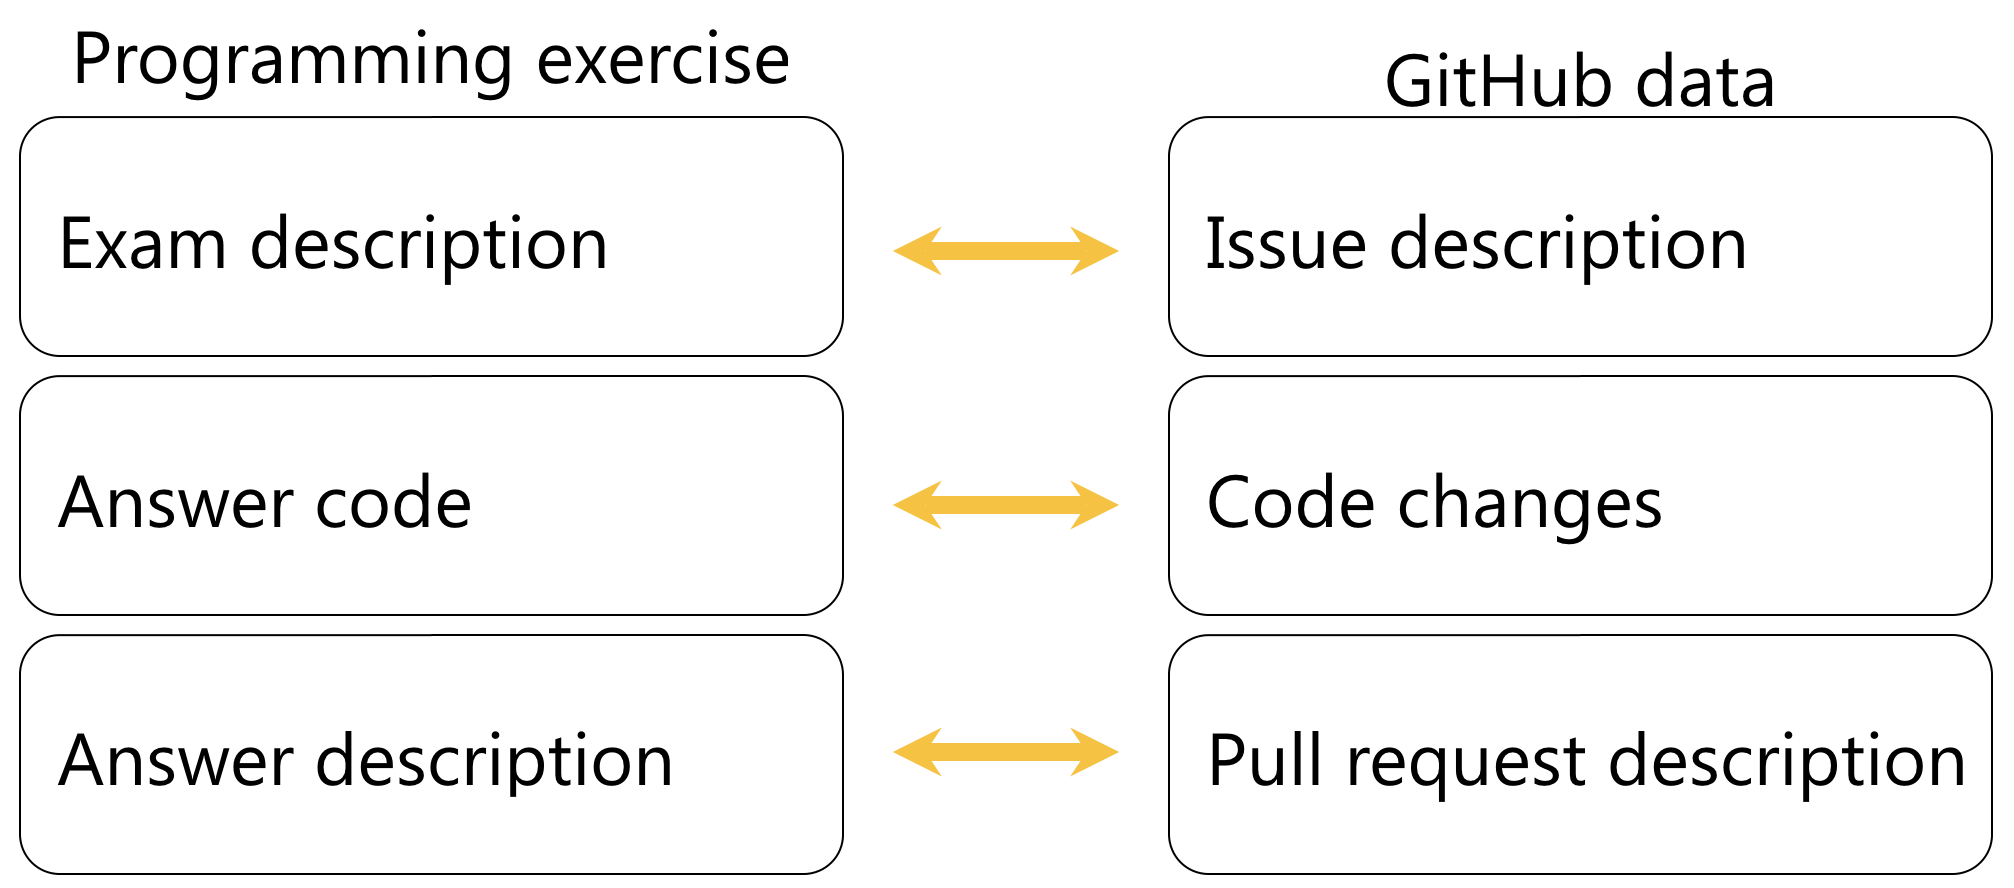
\includegraphics[width=0.9\columnwidth]{system_diagram.png}
    \caption{GitHubのイシューとプルリクエストをプログラミング演習問題へと転用するシステムの概念図.プログラミング演習問題とその解答の説明文を,イシューとプルリクエストの説明文から生成する.さらに解答となるソースコードをプルリクエストのコード変更から生成する.}~\label{fig:system_diagram}
\end{figure}

現実のソフトウェア開発において行われたソースコードの変更データを収集するために,本研究ではソフトウェア開発を管理するウェブ上のプラットフォームであるGitHubのイシューとプルリクエストを使用する.
GitHubが提供するイシューは,ソフトウェア開発における課題を登録し管理する機能である.
イシューを導入することにより,新機能開発や修正すべきバグといった対応すべき課題を開発チーム内にて円滑に共有することが可能となる.
イシューはタイトル・説明文・ラベルなどの情報から構成される.
GitHubのプルリクエストと呼ばれる機能は,イシューを解決するためのコード変更を管理する機能である.
プルリクエストはタイトルや説明文などのイシューと同様の情報に加えて,イシューを解決するためのコード変更の情報から構成される.

多くのソフトウェア開発者がGitHubを利用しており,2016年9月から1年の間に約1200万件のイシューが作成された~\footnote{\url{https://octoverse.github.com/}}.
従ってGitHubには実践的なソースコード変更の膨大なデータが蓄積されており,それらからプログラミング演習問題を生成し提供することで,より実践的な情報技術の習得を支援することができると考えられる.
本研究が提案するイシューとプルリクエストをプログラミング演習問題へと転用するシステムの概念図を図\ref{fig:system_diagram}に示す.
イシューの説明文は対応すべきソフトウェア開発の課題を説明し,その課題を解決するために必要なコード変更はプルリクエストに含まれている.
プログラミング演習問題も同様に,解答すべき課題の説明と,その解答となるソースコードから構成される.
従って,イシューとプルリクエストからプログラミング演習問題に適した情報を抽出することで,半自動的にプログラミング演習問題を生成することができると考える.


\section{データ収集とヒューリスティクスによる事前処理}

% Our goal is to create programming exercises using issues and code diffs on GitHub, and provide learning experience grounded to real development.
本研究の目的は,GitHubのイシューとプルリクエストを転用することで,実際のプログラミング開発で行われたコード変更を演習問題として提供することにある.
% However, not all the issues and code diffs available on GitHub are appropriate for exercise use.
しかし,GitHub上の全てのイシューやプルリクエストが演習問題への転用に適しているとは限らない.
% For instance, issues may contain lengthy code revisions.
例えば説明のないイシューや,リポジトリに関する専門的な知識を必要とするプルリクエストは,学習者にとって理解することが難しいことが想定される.
% \masaki{例えば説明のないイシューや,リポジトリに関する専門知識を含むプルリクエストは,学習者にとって理解することが難しい.}{「説明のない」がどこまでかかるのか最初分からなかったので,イシューやの後に読点があった方が良いかも?}
% Issues without descriptions would be difficult for a third person to understand their objectives.
% Exercises that require special knowledge about a project or are unnecessarily complex would be inappropriate as well.

% Because of an enormous number of issues and code diffs on GitHub, we performed screening before performing classification.
そこで本研究では,GitHub上の公開されているイシューとプルリクエストのうち,プログラミング演習問題に転用できると考えられるものを抽出するため,以下の5つのヒューリスティクスを用いた.
\begin{enumerate}
\item[H1] \textbf{リポジトリ外部の開発者でも対応可能と明示的に指定されているイシューであること}: この情報がイシューに対して明示的に与えられていることは,コード変更に必要な情報が全てイシュー内で提供されていると想定できるため.
\item[H2] \textbf{プルリクエストに含まれるコード変更が50行以下であること}: 極端に長いコード変更は演習問題として不適切であるため.
\item[H3] \textbf{プルリクエストのコード変更が1ファイルのみにて行われていること}: 複数のファイルにまたがるコード変更は各ファイルの役割などリポジトリ特有の知識を必要とする可能性が高いため.
\item[H4] \textbf{イシューが説明文を含むこと}: 説明文をプログラミング演習問題の問題文として利用するため,その情報がないイシューは不適切であるため.
\item[H5]  \textbf{イシューが閉じられており,関連するプルリクエストがマージされていること}: マージはコード変更が開発チームで認められたことを示すものであり,コード変更が適切であることを示すと考えられるため.
\end{enumerate}

\begin{figure}[t]
    \begin{tabular}{c}
      %-------------------------------
      \begin{minipage}[t]{0.5\columnwidth}
        \centering
        
        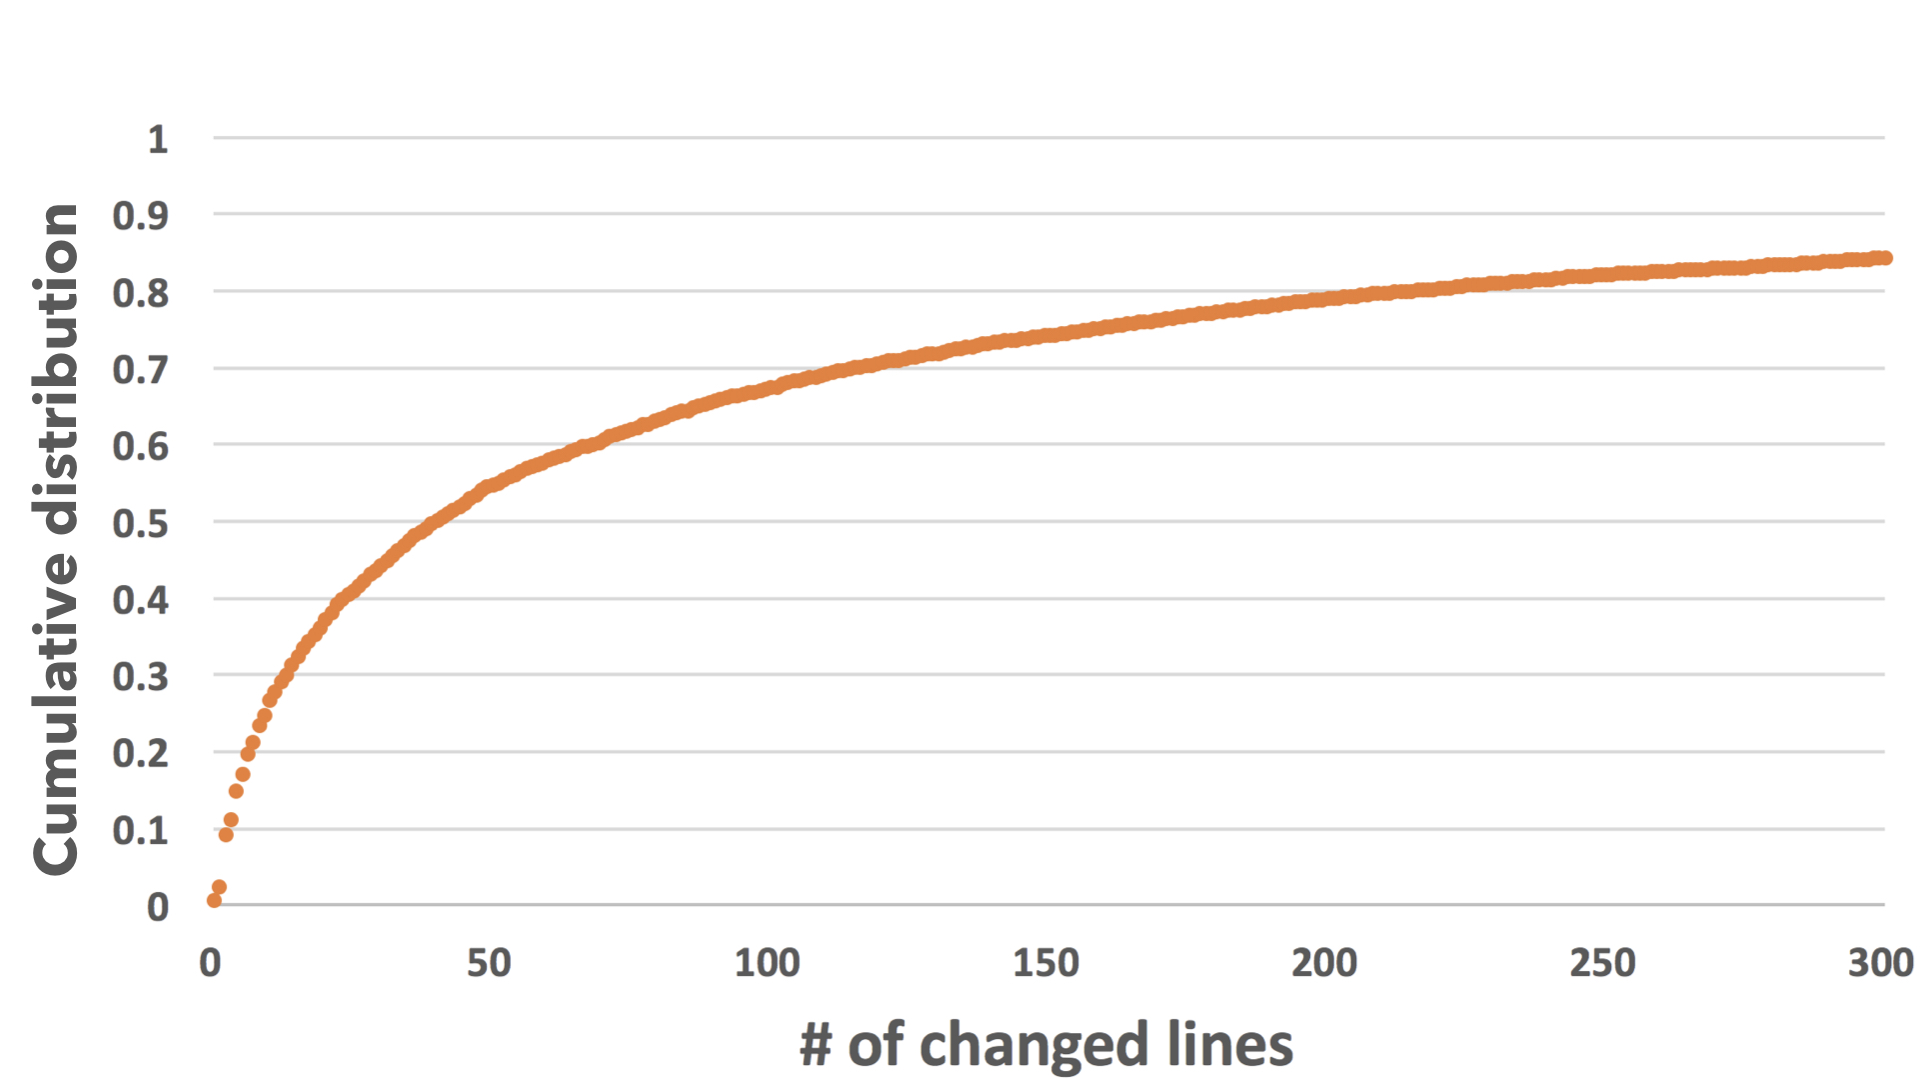
\includegraphics[width=0.95\columnwidth]{realcode_histogram_changed_lines.jpeg}
        \subcaption{コードの変更行数の累積分布.}~\label{fig:histogram_changes}
      \end{minipage}
      
      \hspace{0.05cm}
      
      %------------------------------
      \begin{minipage}[t]{0.5\columnwidth}
        \centering
        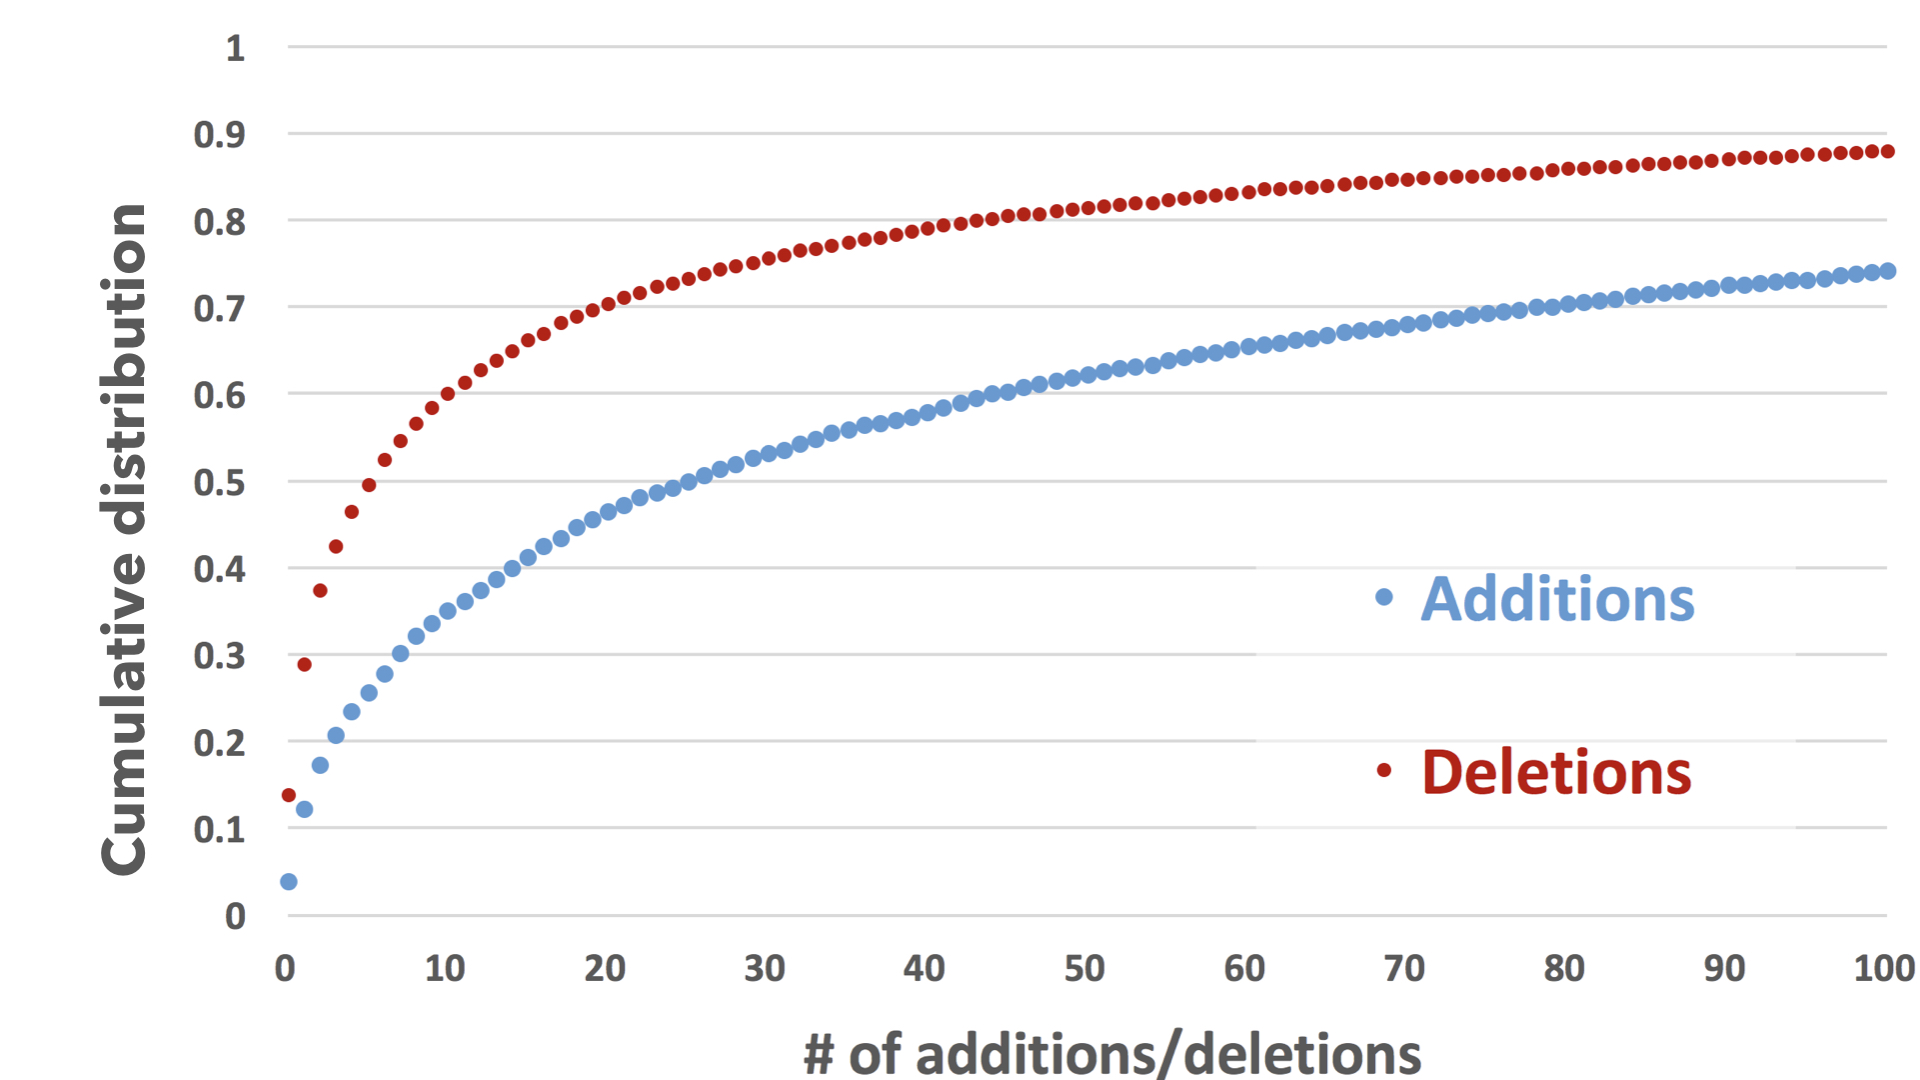
\includegraphics[width=0.92\columnwidth]{realcode_histogram_add_del.jpeg}
        \subcaption{コードの追加および削除行数の累積分布.}~\label{fig:histogram_adds_dels}
      \end{minipage}
      
      \\
      \vspace{-0.5cm}
      
      %------------------------------
      \begin{minipage}[t]{0.5\columnwidth}
        \centering
        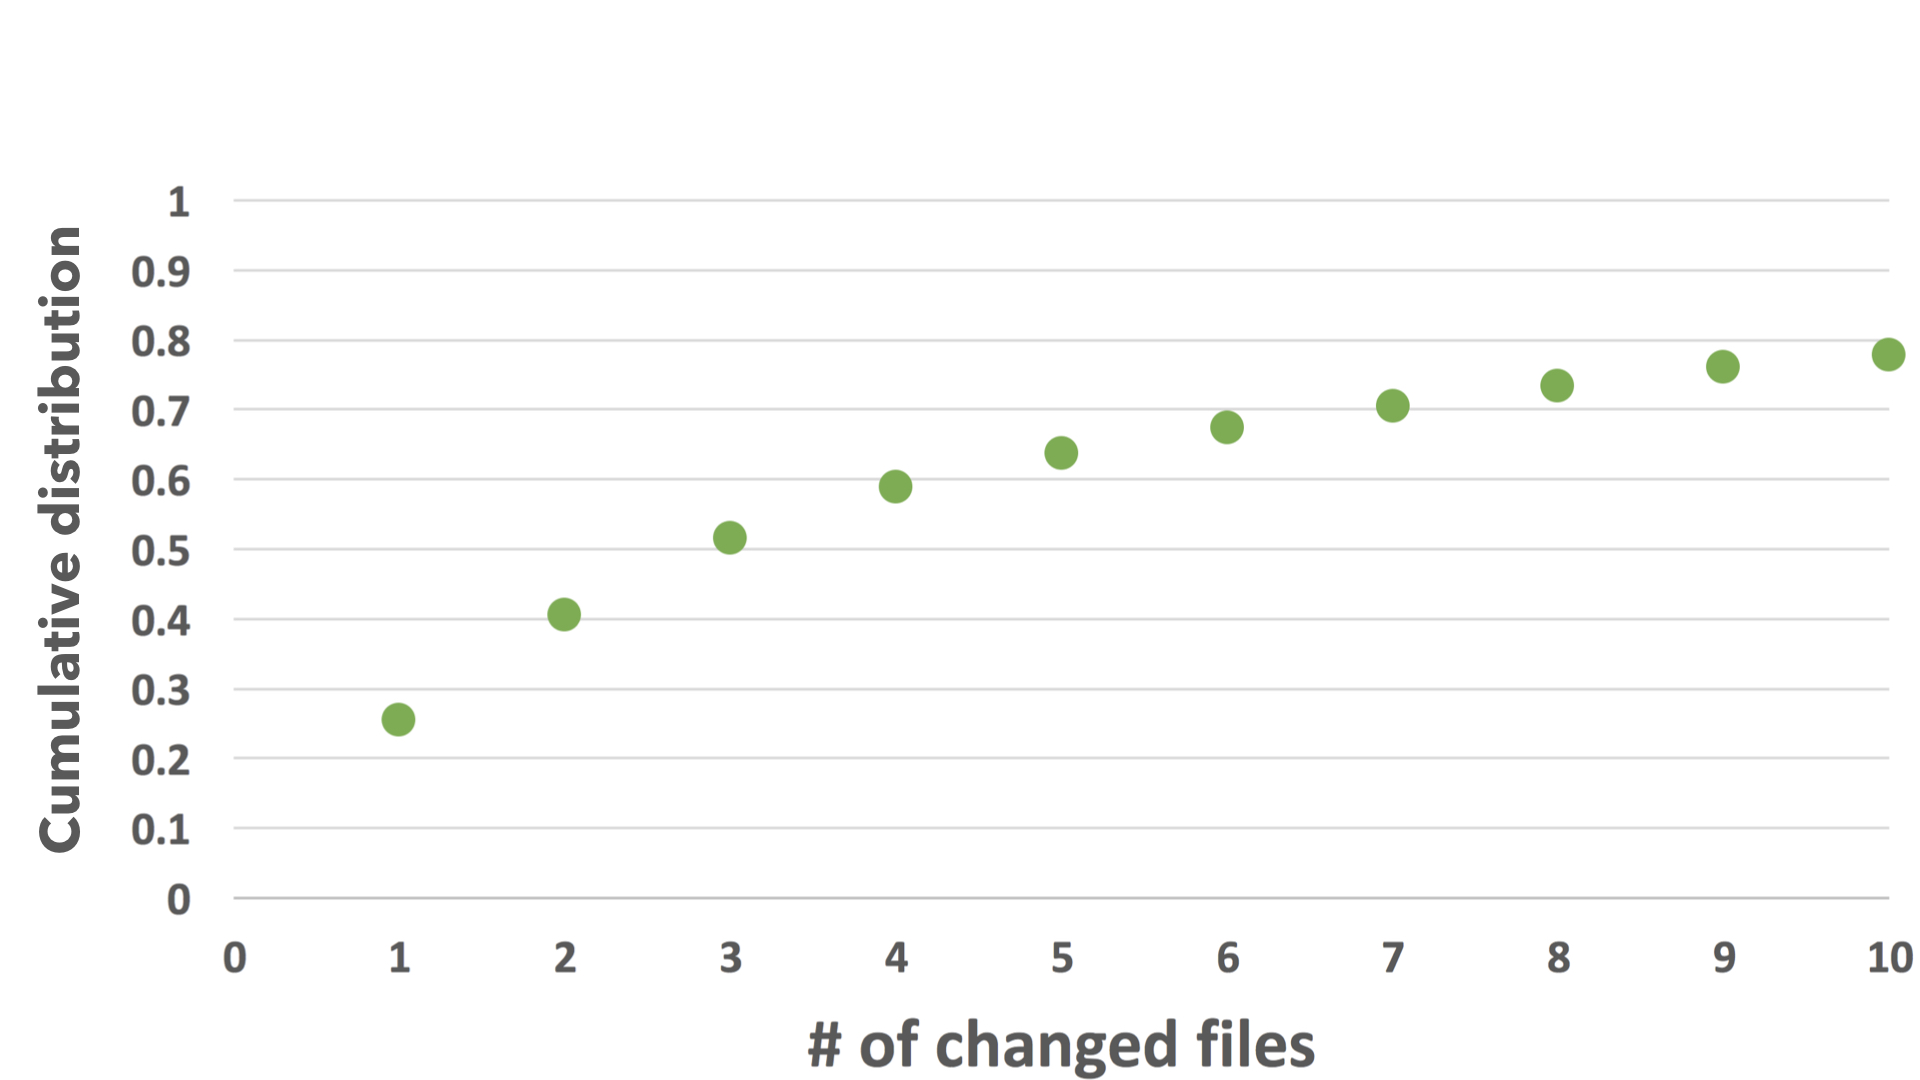
\includegraphics[width=1.0\columnwidth]{realcode_histogram_changed_files.jpeg}
        \subcaption{変更ファイル数の累積分布.}~\label{fig:histogram_changed_files}
      \end{minipage}
     
    \end{tabular}
    \caption{プルリクエストによって変更されたコード変更の行数,追加および削除行数,および変更ファイル数の累積分布.}
\end{figure}

Up for grabs\footnote{\url{http://up-for-grabs.net}}というウェブサイトでは,リポジトリ外部の開発者であっても取り組むことができるイシューを列挙している.
我々はこのウェブサイトが掲載しているラベル(例えば``good first issue''や``help-wanted'')が付けられているイシューのみを利用することで,H1を適応することとした.
また,データ収集時にクエリを使用することで,H4とH5に対応した.
その結果,2018年3月12日の時点で更新が新しい順に3,000件のリポジトリから,H1,H4,H5を満たすイシューと関連するプルリクエストを取得した.
% 成果輪講の話
次に,H2とH3を満たすイシューがどの程度存在するのかを検証するために,収集したプルリクエストにて行われたコードの変更行数の分析を行った.
プルリクエスト内にて変更された行数の累積分布を図\ref{fig:histogram_changes}に,追加・削除された行数の累積分布を図\ref{fig:histogram_adds_dels}に,変更されたファイル数の分布を図\ref{fig:histogram_changed_files}に示す.
以上の分析により,GitHubから収集したイシューと関連するプルリクエストのうち6,381件(1.6\%)がH2とH3を満たすことが明らかとなった.
それらのイシューを抽出することでデータセットを構築した.
% そしてそれらのイシューにH4とH5を適用した結果,6,381件のイシューと関連するプルリクエストを抽出した.

% Data collecting
%%%%%%%%%%%%%%%%%%%


\begin{figure}[tb]
    \centering
    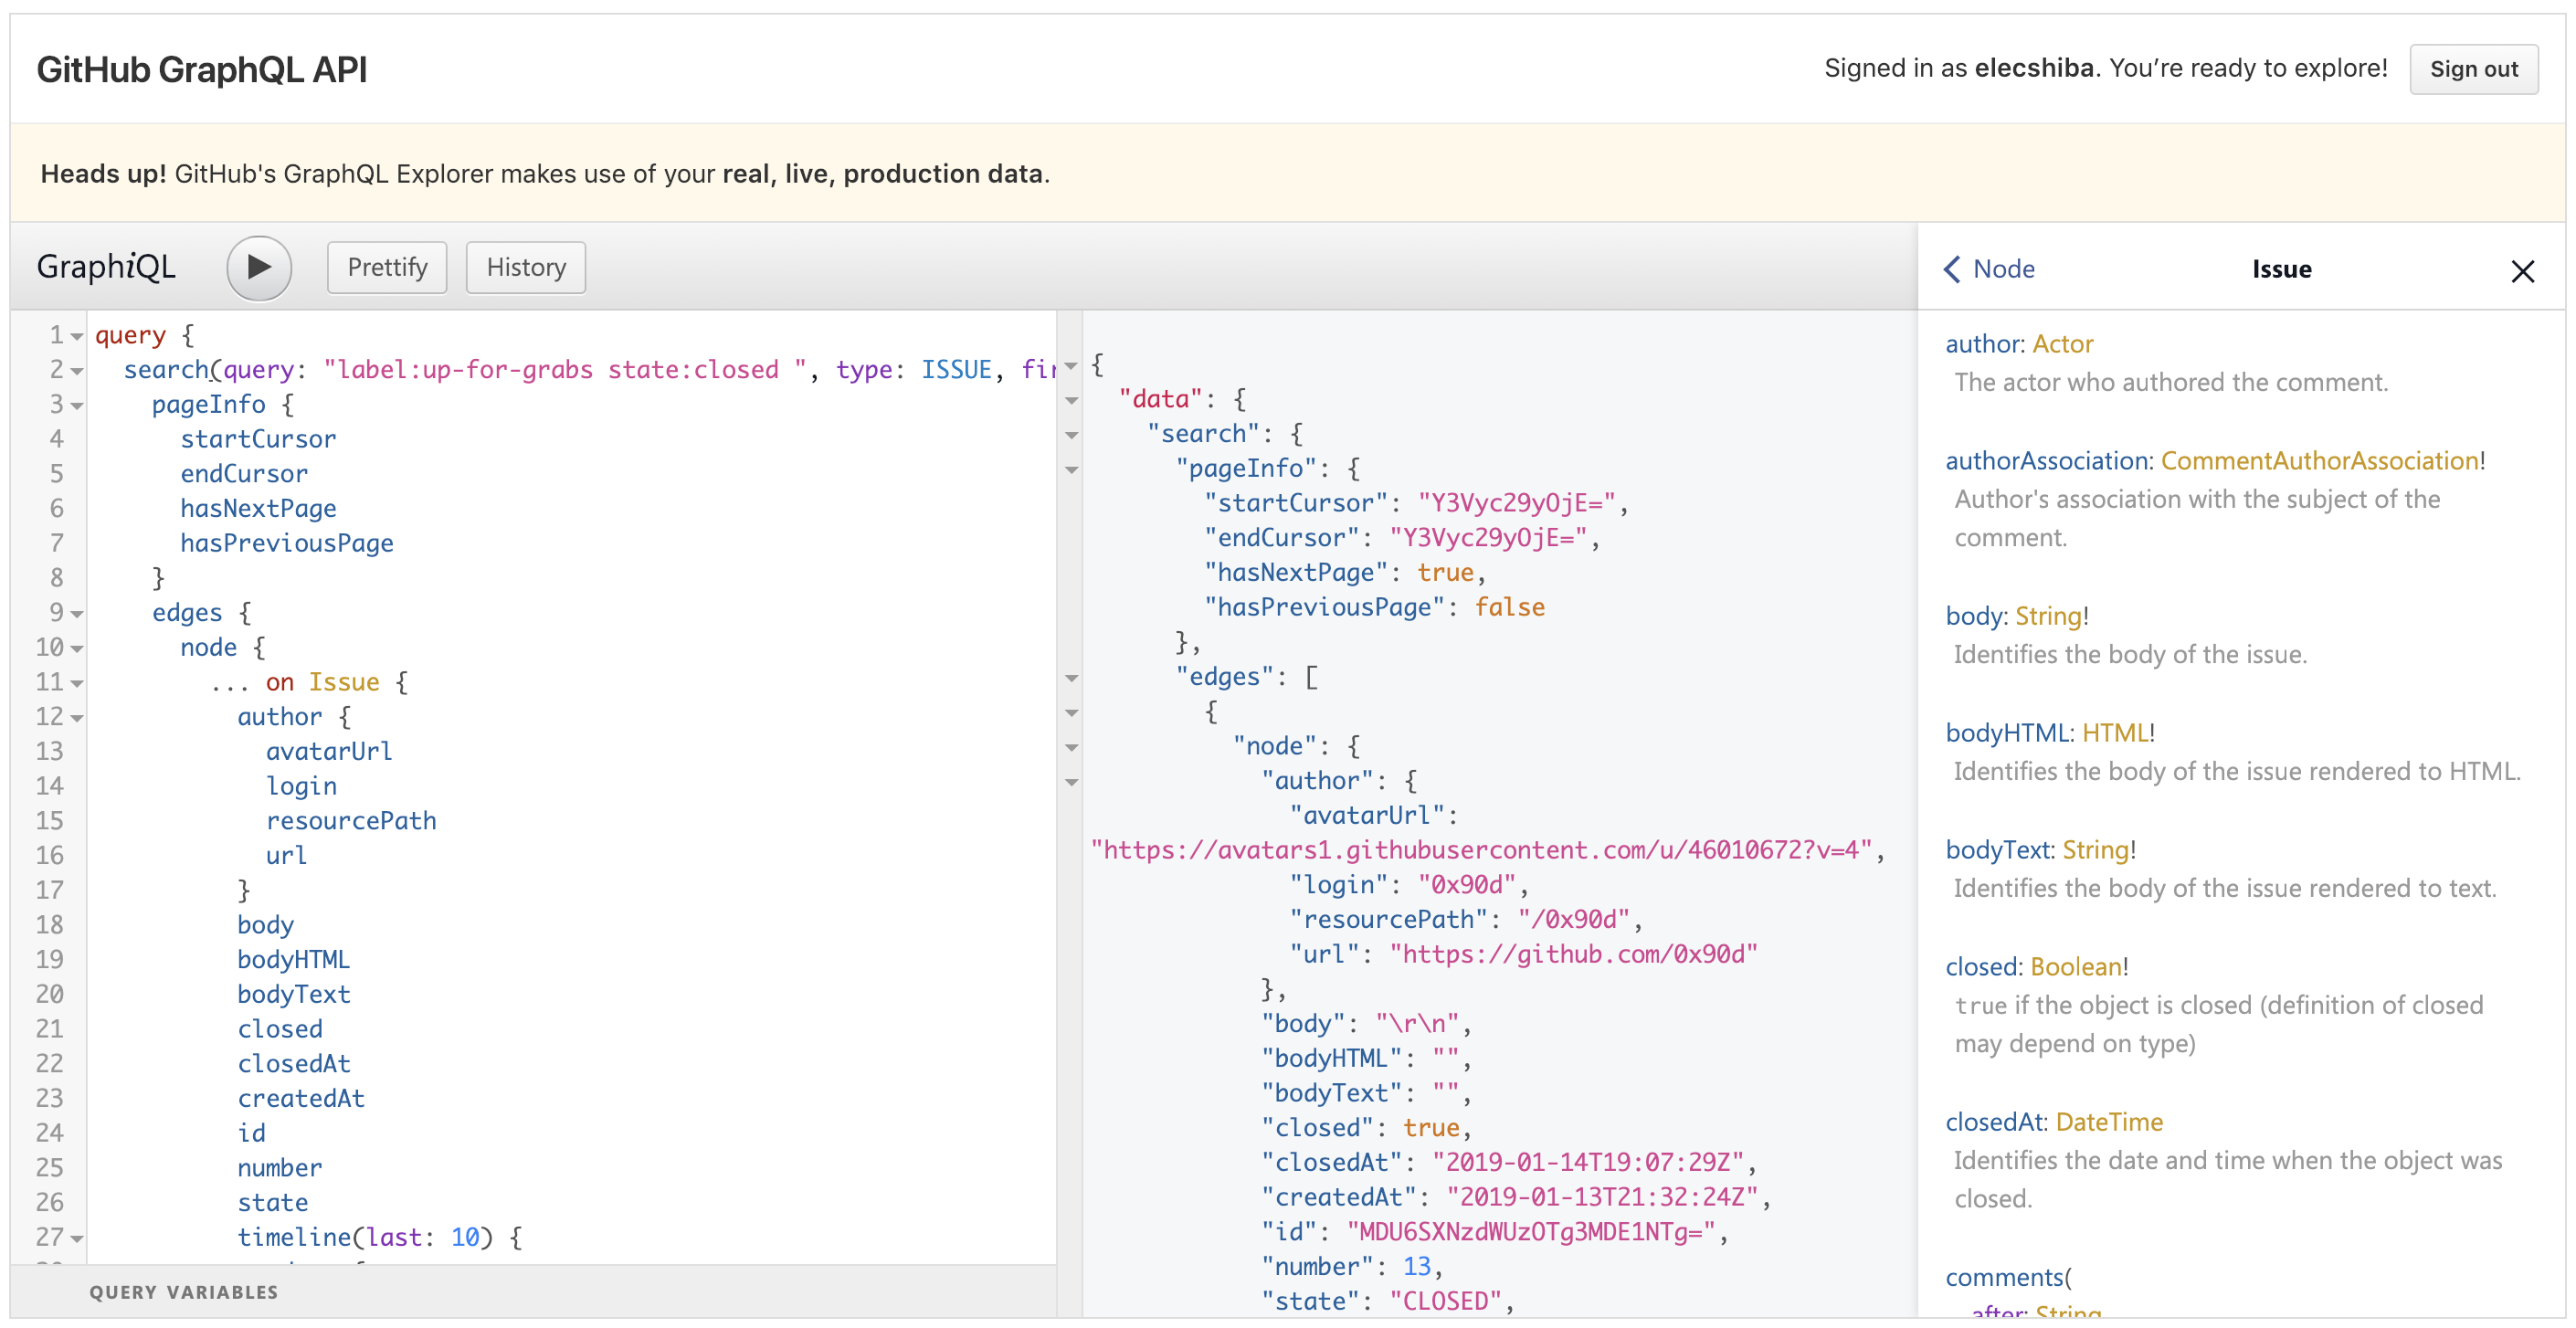
\includegraphics[width=1.0\columnwidth]{GitHub_api_explorer.png}
    \caption{GitHub GraphQL API Explorerにてデータ収集用のクエリを実装している様子.左のエディタ上で実装したクエリを実行した結果が中央に表示されている.また,使用可能なスキーマやフィールドのドキュメントを右側のパネルで閲覧できる.}
    \label{fig:GitHub_api_explorer}
\end{figure}


\begin{table}[t]

  \centering
  \caption{GitHubから収集したデータの構造.}
  \label{table:format_collected_GH_data}
    
  \begin{tabular}{l | c | c } \Xhline{3\arrayrulewidth}
      名前 & 型 & 説明 \\ \hline \hline
      author & json & ユーザ名やユーザページのURLなど\\
      body & string & イシューの説明文  \\
      bodyHTML & string & HTML表記でのイシューの説明文 \\
      comments & [json] & コメントの本文や作成者の情報など \\
      createdAt & datetime & イシューが作成された日時 \\
      labels & [json] & イシューに付与されているラベルに関する情報 \\
      repository & json & リポジトリ名やURL,主要な開発言語など\\  
      state & string & イシューの状態(open,closedなど) \\
      pullRequest & json & プルリクエストの説明文やコード変更量など \\
      title & string & イシューのタイトル \\
      url & string & イシューのURL \\
      
      \Xhline{3\arrayrulewidth}
  \end{tabular}
\end{table}

GitHubからのデータ収集にはGitHub GraphQL~\footnote{\url{https://developer.github.com/v4/}}を使用した.
GraphQLではデータの構造とフィールドを指定することで,必要な情報のみを取得することができる.
また,イシューに関連するプルリクエストといった,関連する異なるオブジェクトをも1クエリで取得することができるという特徴をもつ.
図\ref{fig:GitHub_api_explorer}にGitHub GraphQL API Explorer~\footnote{\url{https://developer.github.com/v4/explorer/}}にてクエリを実装している様子を,表\ref{table:format_collected_GH_data}にデータ収集にて使用したデータ構造を示す.
型がjsonの項目については,その項目に関する必要な情報がネスト形式で記述されている.

\begin{figure}[t]
  \centering
  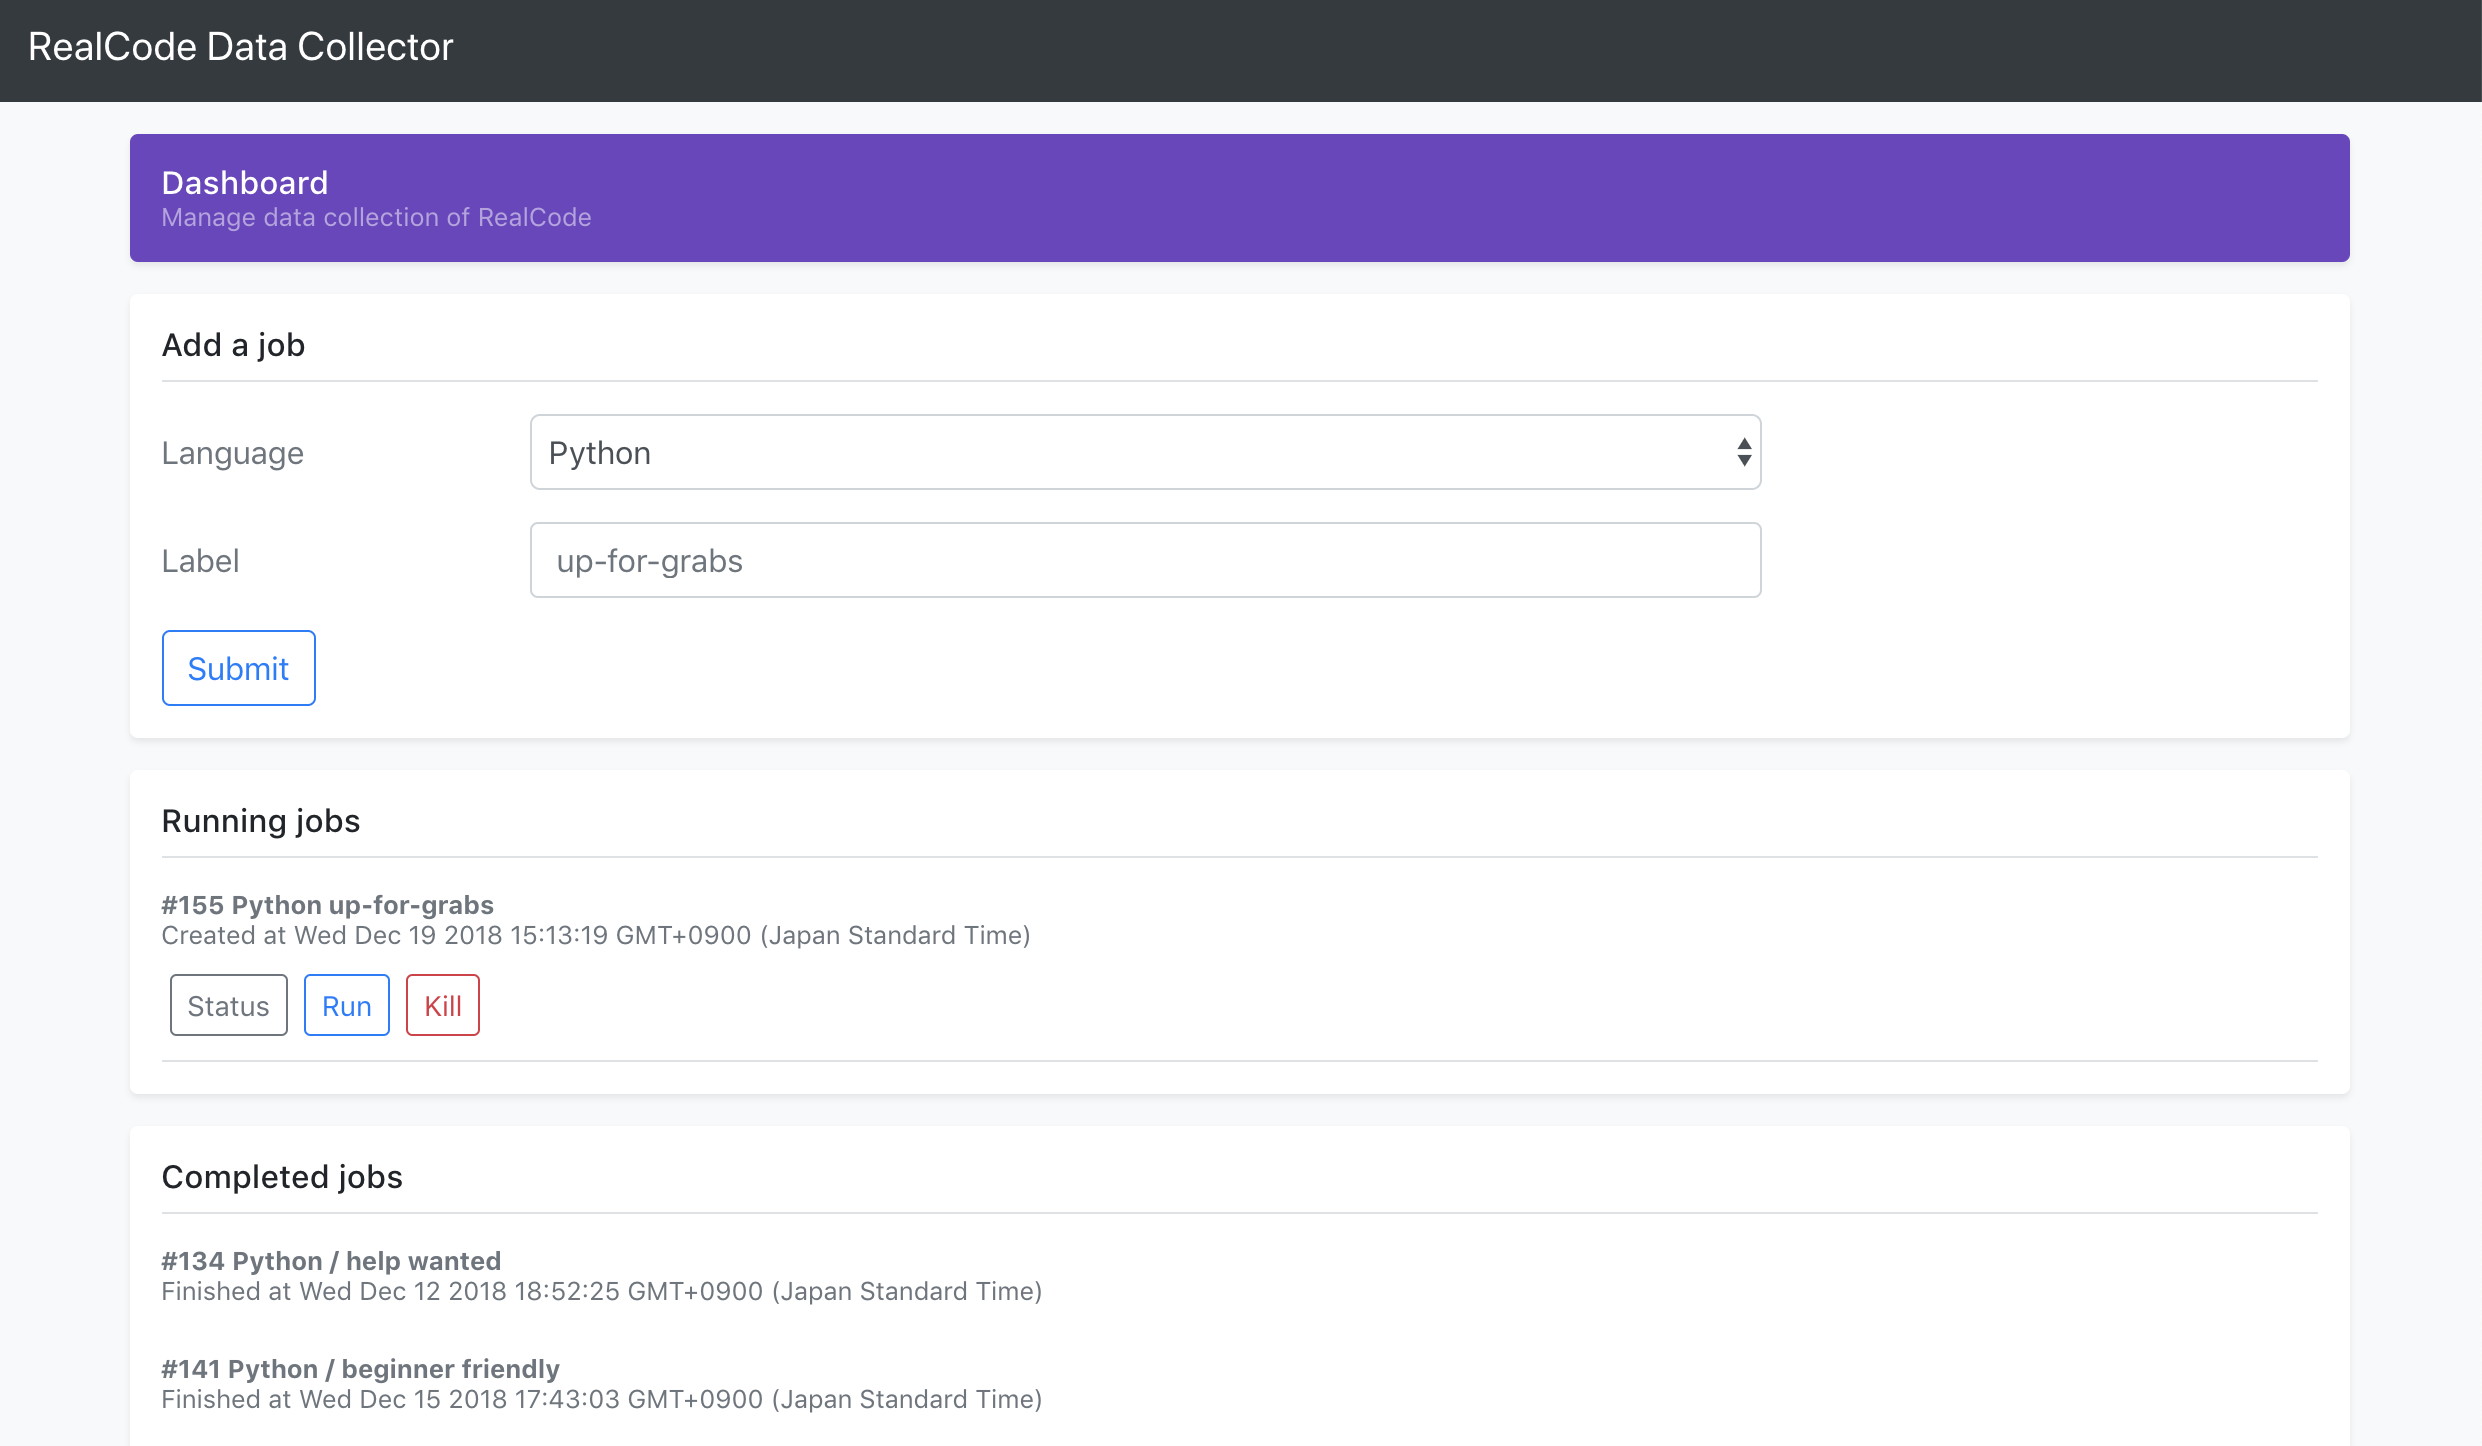
\includegraphics[width=1.0\columnwidth]{realcode-data-collector-screenshot.png}
  \caption{RealCode用のデータ収集管理画面.``Add a job''にてプログラミング言語とイシューのラベルを指定すると,該当するGitHubのデータの収集がジョブとしてバックグラウンドで実行される.実行中のジョブは``Running jobs''に表示され,ジョブの現在の状態を確認できる.完了したジョブは``Completed jobs''に表示される.}
  \label{fig:realcode-data-collector}
\end{figure}

図\ref{fig:realcode-data-collector}に,GitHubからのデータ収集を管理するために開発したシステムのインターフェースを示す.
``Add a job''というタイトルのフォームにて収集するデータのプログラミング言語とイシューのラベルを指定することで,バックグラウンドにてデータ収集のジョブを実行する.
バックグラウンドでジョブを実行するためにKue\footnote{\url{https://github.com/Automattic/kue}}というライブラリを,ジョブの状態を管理するためにRedis\footnote{\url{https://redis.io/}}というインメモリDBを使用している.
実行中のジョブは図\ref{fig:realcode-data-collector}の``Running jobs''に,完了したジョブは``Completed jobs''にそれぞれ表示されている.

GraphQLによりイシューと関連するプルリクエストの情報を抽出することができるが,プルリクエストにて行われた実際のコード変更データはGraphQLからは取得することができない.
GraphQLから収集したイシューについて,gitコマンドを用いて関連するリポジトリとコード変更履歴をクローンし,変更前と変更後のバージョンのコードを比較することでコード変更データを抽出した.
また,Pythonからgitコマンドを実行する際にはGitPython~\footnote{\url{https://gitpython.readthedocs.io/en/stable/}}を使用した.

  
\section{決定木を用いた転用に適したイシューの抽出}

\subsection{データのラベル付け}
前節にて述べたGitHub上のデータ抽出作業により,プログラミング演習問題に転用する上で不適切であると考えられるイシューおよびプルリクエストを取り除くことができた.
しかし,抽出されたデータから作られた演習問題がすべて適切であるとは限らない.
例えばソースコード中のコメントを修正するような演習問題は,プログラミング言語の学習において学べることは非常に小さい.
そこで我々は妥当でないプログラミング演習問題を生成し得るイシューを除去するために,機械学習を用いた分類器を実装することとした.
%また,分類器の学習に必要なデータセットを構築するために,学生によるラベル付けを行った.

% Although our screening filtered out issues clearly unusable for our purpose, it is still unknown whether generated exercises would offer valid problems.
% We thus decided to create a classifier to remove issues and code diffs that would result in invalid exercises.
% To this end, we conducted an experiment to collect human ratings.

分類器の実装にあたり,イシューから転用した演習問題がプログラミング演習問題として成立するかどうかの評価を行い,教師あり学習におけるラベルを生成することとした.
まず,事前処理後のデータに修正を加えずに,イシュー内の説明文とコード変更をそれぞれ問題文,解答コード例とするプログラミング演習問題を生成した.
それぞれの演習問題に対し,「与えられた演習問題は,問題として成立していた.」かを,Pythonの授業を大学で受講した経験がある10人の学生(PA1--10)に5段階で評価してもらった(1: 全く同意しない -- 5: 強く同意する).
各実験参加者には時間の許す限りできるだけ多くの演習問題の評価を行ってもらうように指示した.
評価の結果,少なくとも2人の実験参加者が評価を行ったイシューが211件得られた.

% We recruited 10 students (PA1--10) who had taken at least one Python class at their universities.
% During the experiment spanning for three days, we asked the participants to solve at least 50 exercises generated by our system.
% For each exercise, the participants were asked to response to a 5-Likert scale question of ``This was a valid programming exercise.'' (1=Strongly disagree -- 5=Strongly agree).
% %We offered approximately 45 USD in local currency as a compensation at the end of the experiment.
% The participants were also encouraged to solve as many exercises as possible with an incentive of additional compensation for the top three contributors.
% As a result, we collected 211 exercises that contain ratings from 2 participants.

211件のイシューに対して,得られた回答の平均値が3.5点以上のイシューをプログラミング演習問題への転用に適するもの,それ以外を転用に適さないものとした.
その結果,85件の転用に適するイシュー(``repurposable")と,126件の転用に適さないイシュー(``unrepurposable")を得た.

% We took the average value for the two ratings on each exercise.
% We then categorized each exercise to ``valid'' if the average was equal to or higher than 3.5.
% The rest of the exercises were grouped to ``invalid" to make our classification rather conservative.
% After categorization, we had 85 and 126 exercises for the valid and invalid categories, respectively.

\subsection{分類手法}
% 
ラベル付けされたプログラミング演習問題の件数が限られているため,本研究では決定木を用いた分類器を利用することとした.
決定木は分類の工程や結果を可視化することができるため,どの特徴量が分類に有効であるかどうかを議論することが可能となる~\cite{FRIEDL1997399}.

% Data-intensive methods (e.g., deep learning) would be infeasible due to the small size of our dataset. 
% We instead decided to use a decision tree (a Classification and Regression Tree) for our classification.
% A decision tree also visualizes classification process, and we can examine what features would contribute to accurate classification.

はじめに我々はunrepurposableと分類されるべきイシューを特定するための次の3つの仮説を立てた.
% \sakaguchi{}{これは上の実験のインタビュー結果からでしょうか?}
\begin{itemize}
\item[\textbf{仮説1}: ] \textbf{コード変更が短すぎる.} コードの変更量が少なすぎるものは含まれている学習すべき内容が少ないと想定されるため.
\item[\textbf{仮説2}: ] \textbf{イシューの説明文が短すぎる,あるいは長すぎる.} 説明文が短いものは問題内容を理解するためには十分な情報が入っていない,長過ぎるものは問題内容を読むこと自体に時間がかかりすぎてしまうと想定されるため.
\item[\textbf{仮説3}: ] \textbf{イシューを取得してきたリポジトリが,リポジトリ外部の開発者向けのイシューを頻繁には作成していない.} このようなリポジトリでは,リポジトリ外部の開発者との連携が少なく,外部の開発者向けのイシューの難易度,説明文の情報量に関する十分な経験がないと考えられるため.
\end{itemize}

% To derive potential features, we first derived the following hypotheses for identifying issues to be removed: H1) A code diff causes syntax errors; H2) A code diff is too short; H3) A description is too long or too short; and H4) The associated repository rarely creates entry tasks for external contributors.

上記の仮説を元に,我々は次の3つの特徴量を作成した.

% The second hypothesis is derived because too short code diff would not hold much information to learn.
% We expect that descriptions in a repository which rarely creates issues for external basic-level contributors may not be easy for non-members to understand.
% Based on these hypotheses, we created the four following features:

\begin{itemize}
% \setlength{\leftskip}{-3mm}
  \item \textit{code\_lines}: コード変更の行数
  \item \textit{desc\_words}: イシューの説明文の単語数
  \item \textit{entry\_issues}: 各リポジトリにおいて外部の開発者向けと指定されているイシューの数
\end{itemize}

% \begin{itemize}
% \setlength{\leftskip}{-3mm}
%   \item \textit{syntax\_error}: 1 if the portion affected by a code diff causes syntax errors, and otherwise 0.
%   \item \textit{code\_lines}: the number of lines in code diffs.
%   \item \textit{desc\_words}: the number of words in issue descriptions.
%   \item \textit{entry\_issues}: the number of entry issues in the same repository. For this feature, we counted issues listed in Up for Grabs for each repository.
% \end{itemize}

%We calculated the value of these features for all labeled issue and code diff data.

決定木の学習においては,過学習を防ぐために決定木の深さを3以下にし,分類されたサンプルが3つ以下の枝については枝刈りを行った.
決定木の精度の評価には10分割交差検証法を採用した.

% We then trained a decision tree with constraining its depth to be three to avoid over-fitting.
% We also pruned trees that applied to fewer than three samples.
% We conducted 10-fold cross validation for performance measurement.



\begin{figure}[t]
	\centering
	\vspace{0.2cm}
  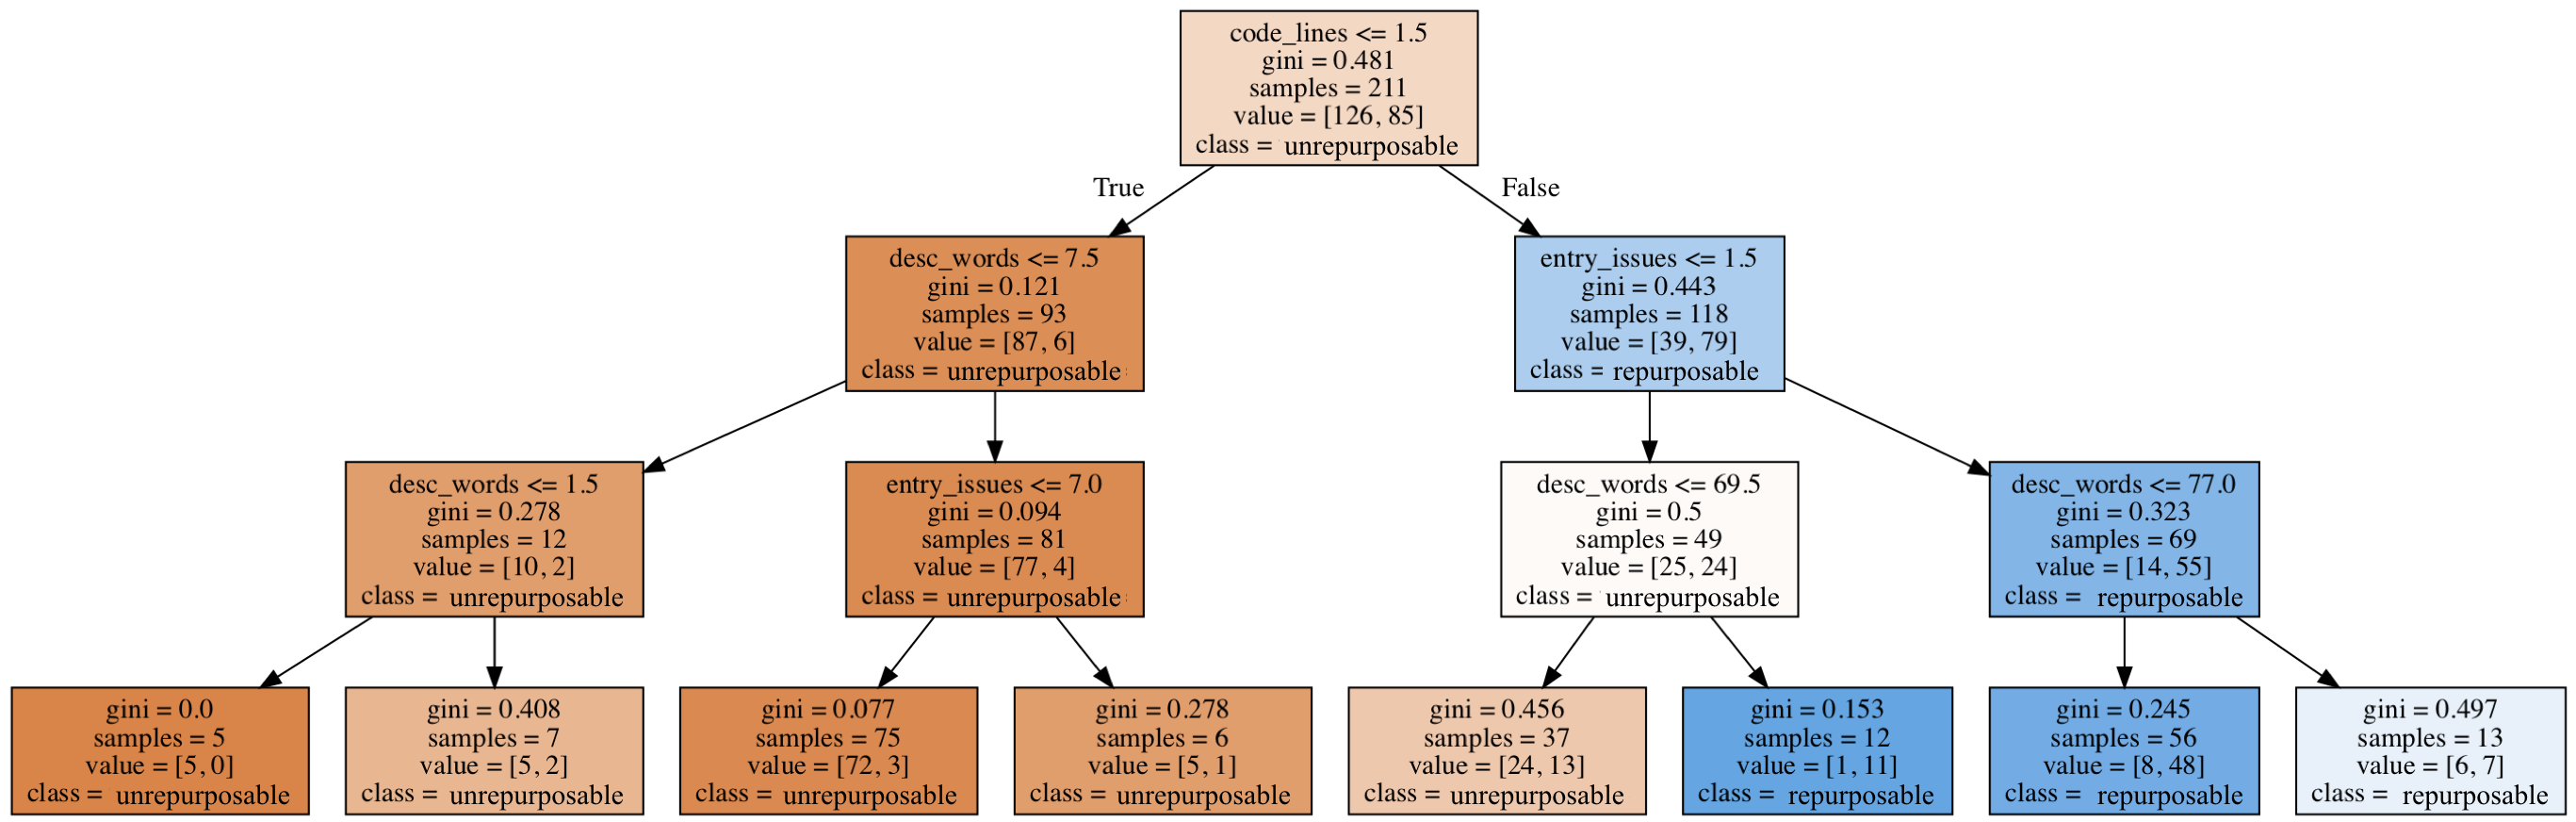
\includegraphics[width=1.0\columnwidth]{graph_20190125.png}
  \vspace{0.2cm}
  \caption{プログラミング演習問題への転用に適するイシュー(``repurposable")と,転用に適さないイシュー(``unrepurposable")を分類する決定木.背景色が青の葉はrepurposableへと,橙の葉はunrepurposableへと分類する.葉の背景色が濃いほど,ジニ係数が小さいことを意味する.}
  \label{fig:dtgraph}
\end{figure}


図\ref{fig:dtgraph}に211件のラベルづけされた全てのイシューを用いて学習させた決定木を示す.
橙はunrepurposable,青はrepurposableとして分類されることを意味する.
10分割交差検証法で識別精度を検証した結果,unrepurposableな演習問題において適合率が0.89,再現度が0.73,repurposableなイシューにおいて適合率が0.71,再現度が0.83であった.
図\ref{fig:dtgraph}が示すように,コード変更の行数を用いた分類が第1段階で行われており,イシューの識別において大きな役割を担っていることが示唆される.
特に,1行のコード変更からなる演習問題の多くがunrepurposableな演習問題として分類されている.
また,\textit{desc\_words}と\textit{entry\_issues}も分類に一定の寄与を示しており,仮説から構築した特徴量がある程度の効果を上げていることが見て取れる.
% Figure~\ref{fig:dtgraph} shows the decision tree trained with all 211 samples.
% Orange and blue represent the ``invalid" and ``valid" classes, respectively.
% This decision tree showed reasonable classification accuracy: precision: 0.89, recall: 0.73 for invalid exercises; and  precision: 0.71, recall: 0.83 for valid exercises.
% It suggests that the numbers of lines in code diffs is the key feature.
% A single-line code diff is likely to result in invalid exercise.
% \textit{desc\_words} and \textit{entry\_issues} offer additional contributions to the classification.
%This decision tree showed reasonable classification accuracy: precision: 0.84, recall: 0.64 for invalid exercises; and  precision: 0.67, recall: 0.83 for valid exercises.
%It suggests that the numbers of lines in code diffs and entry issues in the associated repositories are the key features.
%Valid exercises are likely to have 2--13 lines in code diffs and to be in a repository that has produced multiple entry issues.




図\ref{fig:dtgraph}の深さが1の左の葉では既にジニ係数が0.1207となっており,unrepurposableと分類する純度の高い葉が$\textit{code\_lines}=1$のみの条件により生成できていることが分かる.
この条件では,ソースコード中の1行のタイプミスの修正や,1行のみのコード変更によるバグ修正などの例が確認できた.
そういった演習問題では,プログラミング言語の学習において学べることは非常に小さい,あるいは前後のコードが明示的に与えられない為に解答するうえで必要な背景知識が十分に提示できていないことが多く存在する.
図\ref{fig:dtgraph}に示す分類器は,このようなイシューを正しくunrepurposableと分類できている.

一方で深さが3の右二つの葉では,repurposableと分類されており,かつジニ係数が高くなっている(0.245と0.497).
即ち,unrepurposableと分類されるべき多くのイシューが誤ってrepurposableと分類されてしまっている.
図\ref{fig:dtgraph}を見ると,\textit{code\_lines}が2以上かつ\textit{entry\_issues}が2以上を満たすイシューがこれら右2つの葉に分類されている.
それらの条件を満たすunrepurposableなイシューの例としては,実験参加者にとってあまり馴染みのないソフトウェア(例えば自動デプロイ用のコンソールアプリ)のリポジトリから抽出されたイシューなどがあった.
ウェブアプリやライブラリといったリポジトリの特徴を決定木の特徴量に加えることで,さらに決定木の精度を向上させることができると考えられる.

この決定木を用いたフィルタリングは完全ではないが,F値の平均が0.79の精度でプログラミング演習問題への転用に適さないイシューを取り除くことができており,現在のプロトタイプに導入することとした.
この決定木により,6,381件中の2,592件のイシューと関連するプルリクエストが転用に適すると判断され,現在のRealCodeのシステムにおいてプログラミング演習問題に使用されている.



\section{構築したデータセットの分析}
決定木により転用可能とされたイシューを用いることで,RealCodeのデータセットを構築することができた.
次にデータセットの概要を理解するために,データセットに含まれるリポジトリとイシューの分析を行った.
以下に分析結果とその考察を記す.

\subsection{リポジトリに関する分析結果}

表\ref{table:stats_repos}にデータセットのイシューが属するリポジトリに関する各種統計量を示す.
平均のコミット数・イシュー数・プルリクエスト数がそれぞれ約4337・1188・1022件と,比較的大規模なリポジトリからデータセットが構築されていることが分かる.
またスター数やフォーク数も高いことから,人気があり外部の開発者も実装に貢献しているリポジトリが多く含まれていることが分かる.

\begin{table}[!b]
  \small
  \centering
  \caption{RealCodeのデータセットのリポジトリに関する各種統計量.}
  \label{table:stats_repos}
  \begin{tabular}{c || c | c | c | c | c | c} \Xhline{3\arrayrulewidth}
        & \# of commits & \# of issues & \# of pull requests & \# of languages & \# of forks & \# of stars \\ \hline
        % count & 458 & 466 & 466 & 466 & 466 & 466 & 466 \\
        mean & 4337.33 & 1188.29 & 1022.16 & 4.95 & 780 & 4165.52 \\
        std & 7797.91 & 1728.25 & 1439.18 & 4.36 & 1230.71 & 5645.54 \\
        min & 35 & 5 & 3 & 1 & 1 & 8 \\
        25\% & 727.25 & 239.25 & 191.5 & 3 & 174.25 & 823 \\
        50\% & 1795.5 & 582 & 524 & 4 & 422 & 2405.5 \\
        75\% & 4948.75 & 1422.25 & 1223.25 & 6 & 909.75 & 4806.75 \\
        max & 114532 & 14464 & 15442 & 52 & 13261 & 43610 \\
    \Xhline{3\arrayrulewidth}
\end{tabular}
\end{table}

\begin{table}[!b]
\small
    \centering
    \caption{RealCodeのデータセットの出現頻度が高いリポジトリのトピック100件.}
    \label{table:repo_topic_freq}
    \begin{tabular}{ c | c || c | c || c | c || c | c} \Xhline{3\arrayrulewidth}
        トピック名 & 頻度 &  &  &  &  &  & \\ \hline \hline
        python & 68 & django & 7 & symfony & 5 & jupyter & 4 \\
        javascript & 54 & typescript & 7 & babel & 5 & awesome-list & 4 \\
        react & 18 & game-engine & 7 & automation & 5 & golang & 4 \\
        php & 17 & machine-learning & 7 & browser & 5 & electron & 4 \\
        go & 13 & java & 7 & server & 5 & monitoring & 4 \\
        swift & 13 & html & 7 & documentation & 5 & dotnet & 4 \\
        android & 13 & database & 6 & performance & 5 & csharp & 4 \\
        nodejs & 12 & gamedev & 6 & awesome & 5 & package-manager & 4 \\
        ios & 11 & data-science & 6 & mongodb & 5 & list & 4 \\
        linux & 11 & kubernetes & 6 & visualization & 5 & eslint & 4 \\
        docker & 10 & api & 6 & theme & 5 & metrics & 4 \\
        ruby & 9 & github & 6 & testing & 5 & rest & 4 \\
        rust & 9 & security & 6 & sass & 5 & blockchain & 4 \\
        c-sharp & 9 & rails & 6 & git & 5 & ecommerce-platform & 3 \\
        containers & 9 & tls & 6 & cms & 4 & macos & 3 \\
        css & 8 & redux & 6 & artificial-intelligence & 4 & cpp & 3 \\
        web & 8 & flask & 6 & es6 & 4 & swift-library & 3 \\
        python3 & 8 & terminal & 6 & irc & 4 & privacy & 3 \\
        c-plus-plus & 8 & cli & 6 & laravel & 4 & cncf & 3 \\
        framework & 8 & scala & 6 & shell & 4 & selenium & 3 \\
        wordpress & 8 & game-development & 5 & visual-studio & 4 & web-framework & 3 \\
        http & 8 & github-api & 5 & ecommerce & 4 & development & 3 \\
        c & 7 & linter & 5 & functional-programming & 4 & plotting & 3 \\
        node & 7 & gui & 5 & open-source & 4 & rest-api & 3 \\
        windows & 7 & react-native & 5 & p2p & 4 & kotlin & 3 \\
        \Xhline{3\arrayrulewidth}
    \end{tabular}
\end{table}

次にデータセット中のリポジトリが何を開発しているのかを理解するために,リポジトリに付与されているトピックのうち出現頻度が高い100件を抽出した(表\ref{table:repo_topic_freq}).
上位に``python''や``javascript''といったプログラミング言語名が多く現れている.
また,``css''や``web''といったウェブや,``ios''や``android''などのモバイル,``docker''や``framework''などのソフトウェア管理といった多様なトピックが上位に出現しており,RealCodeのデータセットには様々な目的のリポジトリが含まれていることが分かる.
加えて,``react''や``nodejs''といったフレームワーク名もトピック名として多く指定されている.
RealCodeが出題する演習問題のトピックを指定することができるようになれば,ユーザが学習したい内容に応じて演習問題を提供できるようになると考えられる.

\begin{table}[!b]
 \small
  \centering
  \caption{RealCodeのデータセットのイシューに関する各種統計量.}
  \label{table:stats_issues}
  \begin{tabular}{c || c | c | c | c | c } \Xhline{3\arrayrulewidth}
        & \# of additions & \# of deletions & \# of commits & \# of comments & \# of changed lines \\ \hline \hline
        mean & 4.5 & 1.79 & 1.12 & 2.02 & 5.69 \\
        std & 5.44 & 1.53 & 0.12 & 2.6 & 5.65 \\
        min & 0 & 0 & 1 & 0 & 0 \\
        25\% & 1 & 0 & 1 & 1 & 2 \\
        50\% & 7 & 3 & 1 & 1 & 4 \\
        75\% & 11 & 6 & 1 & 3 & 7 \\
        max & 48 & 8 & 3 & 28 & 50 \\
    \Xhline{3\arrayrulewidth}
\end{tabular}
\end{table}

\begin{table}[!b]
    \small
    \centering
    \caption{コード変更のプログラミング言語の頻度表.} 
    \label{table:issue_lang_freq}
    \begin{tabular}{c | c || c | c || c | c || c | c} \Xhline{3\arrayrulewidth}
        プログラミング言語名 & 件数 &  &  &  &  &  &   \\ \hline \hline
        JavaScript & 336 & Ruby & 34 & Less & 6 & FreeMarker & 2 \\
        Go & 117 & Shell & 33 & Slim & 6 & VimL & 2 \\
        Python & 116 & Jade & 32 & Clojure & 6 & Groff & 2 \\
        C++ & 116 & XML & 29 & HTML+ERB & 5 & F# & 2 \\
        RenderScript & 112 & SCSS & 28 & Limbo & 5 & Lua & 2 \\
        C# & 97 & Scala & 26 & TOML & 5 & IDL & 2 \\
        Hack & 94 & Swift & 24 & Handlebars & 4 & Objective-C++ & 2 \\
        CSS & 65 & TypeScript & 23 & INI & 4 & NSIS & 2 \\
        JSON & 63 & Twig & 21 & Dart & 4 & Pascal & 2 \\
        HTML & 60 & Kotlin & 16 & AsciiDoc & 4 & PLSQL & 1 \\
        Java & 57 & Perl & 15 & Cucumber & 4 & Makefile & 1 \\
        Text & 48 & PowerShell & 8 & CMake & 4 & Erlang & 1 \\
        C & 44 & Haml & 7 & Stylus & 4 & desktop & 1 \\
        YAML & 37 & CoffeeScript & 6 & SVG & 4 & Gradle & 1 \\
        reStructuredText & 35 & JSX & 6 & OCaml & 3 & HTML+PHP & 1 \\

        \Xhline{3\arrayrulewidth}
    \end{tabular}

\end{table}

\subsection{イシューに関する分析結果}

次に表\ref{table:stats_issues}にデータセットのイシューに関する各種統計量を示す.
平均の追加行数・削除行数がそれぞれ約4.5・1.8行と,比較的小さいコード変更から構成されていることが分かる.
また追加行数が削除行数よりも大きいことから,RealCodeのデータセットの多くが主に新規にコードを追加したイシューであることが分かる.

次にコード変更がどのプログラミング言語が行われているかを分析した(表\ref{table:issue_lang_freq}).
計60のプログラミング言語(但し``HTML+ERB''のような組み合わせも含む)がRealCodeのデータセット中に存在し,多様なプログラミング言語の学習支援に対応できる可能性があることが分かる.
また,``JavaScript''や``Python''といった人気のプログラミング言語\footnote{\url{https://octoverse.github.com/projects.html}}が上位にあることが分かる.
一方で,``JSON''や``Text''といったデータや文章を記述するための言語も上位に位置している.
それらの言語で行われたコード変更の多くがリポジトリのドキュメントの更新であり,プログラミング学習においては妥当でないデータである可能性が高い.
今回行った決定木にはプログラミング言語に関する特徴量が含まれていなかったため,このようなデータを除去できていないと考えられる.

次にデータセット中のイシューが作成された目的を理解するために,イシューに付与されているラベルのうち出現頻度が高い100件を抽出した(表\ref{table:issue_label_freq}).
``help wanted''や``good first issue''といった,外部の開発者を積極的に歓迎するためのラベルが多く表れている.
また``enhancement''といった新規機能開発や``Bug''といったバグ修正など,データセット中のイシューには様々な開発目的があることが分かる.
リポジトリのトピックと同様に,同じ意味をもつラベル(例えば``bug''と``kind/bug''など)を集約することができれば,ユーザの好みに応じて提示する演習問題を限定できるようになると考える.


% リポジトリのトピックと同様に,演習問題のラベルを指定できるようになればユーザの適応的なプログラミング学習を支援できる可能性がある.
% 一方で現状のデータセット中には非常に多くのラベルが存在するため,ユーザにとってそれらから選択するのは困難である.
% 同じ意味をもつラベル(例,``bug''と``kind/bug''など)を分類することができれば,コード変更の種類を限定した上で演習問題を提示できると考える.

\begin{table}[!b]
    \small
    \centering
    \caption{RealCodeのデータセットの出現頻度が高いイシューのラベル100件.}
    \label{table:issue_label_freq}
    \begin{tabular}{ c | c || c | c || c | c } \Xhline{3\arrayrulewidth}
        ラベル名 & 頻度 &  &  &  &  \\ \hline \hline
        help wanted & 889 & Missing Documentation & 24 & Good first issue & 12 \\
        good first issue & 526 & kind/enhancement & 24 & Priority: High & 12 \\
        bug & 339 & question & 23 & release\_note:enhancement & 12 \\
        enhancement & 224 & Good for New Contributors & 22 & small & 11 \\
        easy & 165 & trivial & 22 & cleanup & 11 \\
        Bug & 154 & welcome contribute & 21 & low-hanging-fruit & 10 \\
        E-easy & 122 & Junior & 20 & cosmetic & 10 \\
        up for grabs & 104 & help-wanted & 20 & component: documentation & 10 \\
        Actionable & 94 & P-low & 20 & C-chore & 10 \\
        low hanging fruit & 84 & in-progress & 19 & priority: 2 - low & 10 \\
        beginner & 79 & Design & 18 & L-rust & 10 \\
        I-bug & 70 & Type: Enhancement & 18 & A-builder & 10 \\
        up-for-grabs & 67 & easy pickings & 18 & type - bug & 10 \\
        Hacktoberfest & 63 & category - doc & 18 & type: bug & 10 \\
        docs & 61 & Status: Available & 17 & v4.1.0 & 10 \\
        Help Wanted & 60 & type: documentation & 16 & minor & 10 \\
        Low-Hanging Fruit & 59 & Type: Bug & 16 & comp: help & 10 \\
        hasPR & 54 & Form & 16 & priority: minor & 10 \\
        documentation & 54 & Documentation & 16 & component/host & 9 \\
        Easy & 53 & Enhancement & 16 & p2 & 9 \\
        Easy Pick & 45 & junior job & 15 & difficulty/newcomer & 8 \\
        I-ui & 40 & difficulty: easy & 15 & ruby 2.0-2.2 & 8 \\
        effort/easy & 38 & UX & 15 & proposal & 8 \\
        first-timers-only & 33 & ui & 15 & JRuby 9000 & 8 \\
        complexity/easy & 31 & Ready for PR & 14 & Console & 8 \\
        C-bug & 30 & A-headers & 14 & Validator & 8 \\
        kind/bug & 29 & Improvement & 14 & broken site & 8 \\
        feature & 27 & type:bug & 13 & Mend It Monday & 8 \\
        PR sent & 26 & easy fix & 13 & Grooming & 8 \\
        hacktoberfest & 26 & Feature & 13 & cmake & 8 \\
        easy-fix & 25 & newbie & 13 & A-studio & 8 \\
        good-first-issue & 24 & kind/documentation & 12 & L-shell & 8 \\
        difficulty: beginner & 24 & core & 12 & ingame/ai & 8 \\
        Priority: Medium & 24 & & & & \\
        \Xhline{3\arrayrulewidth}
    \end{tabular}
\end{table}






\def\vector#1{\mbox{\boldmath $#1$}}

%!TEX root = ../thesis.tex
%*******************************************************************************
%****************************** Forth Chapter **********************************
%*******************************************************************************
\chapter[インターフェース]{インターフェース}
\graphicspath{{Chapters_implementation/Figs/}}



RealCodeは\ref{section:issue-classification}章で転用可能とされたイシューのデータを3種類のインターフェースを通じて演習問題として学習者に提供することができる.
図\ref{fig:interface-selector},~\ref{fig:realcode-mobile}に示すように,システムはデスクトップとモバイルの両方に対応しており,ユーザの柔軟な学習を支援できる~\cite{gassler2004integrated}.
3種類のインターフェースはそれぞれ,単語帳(図\ref{fig:flash}),選択式(図\ref{fig:mcq}),穴埋め式(図\ref{fig:fill})の形式で演習問題を提示する.
RealCodeではイシューの説明文を問題文として,対応するプルリクエストのコード変更を解答コードとして利用している.
現在のRealCodeには一般的なプログラミング言語(例,Python)に加えて,マークアップ言語(例,CSS)や拡張言語(例,Sass),設定言語(例,TOML)を含む60のプログラミング言語の演習問題が用意されている(但し,穴埋め式のインターフェースはPythonのみ).

\begin{figure}[H]
	\centering
  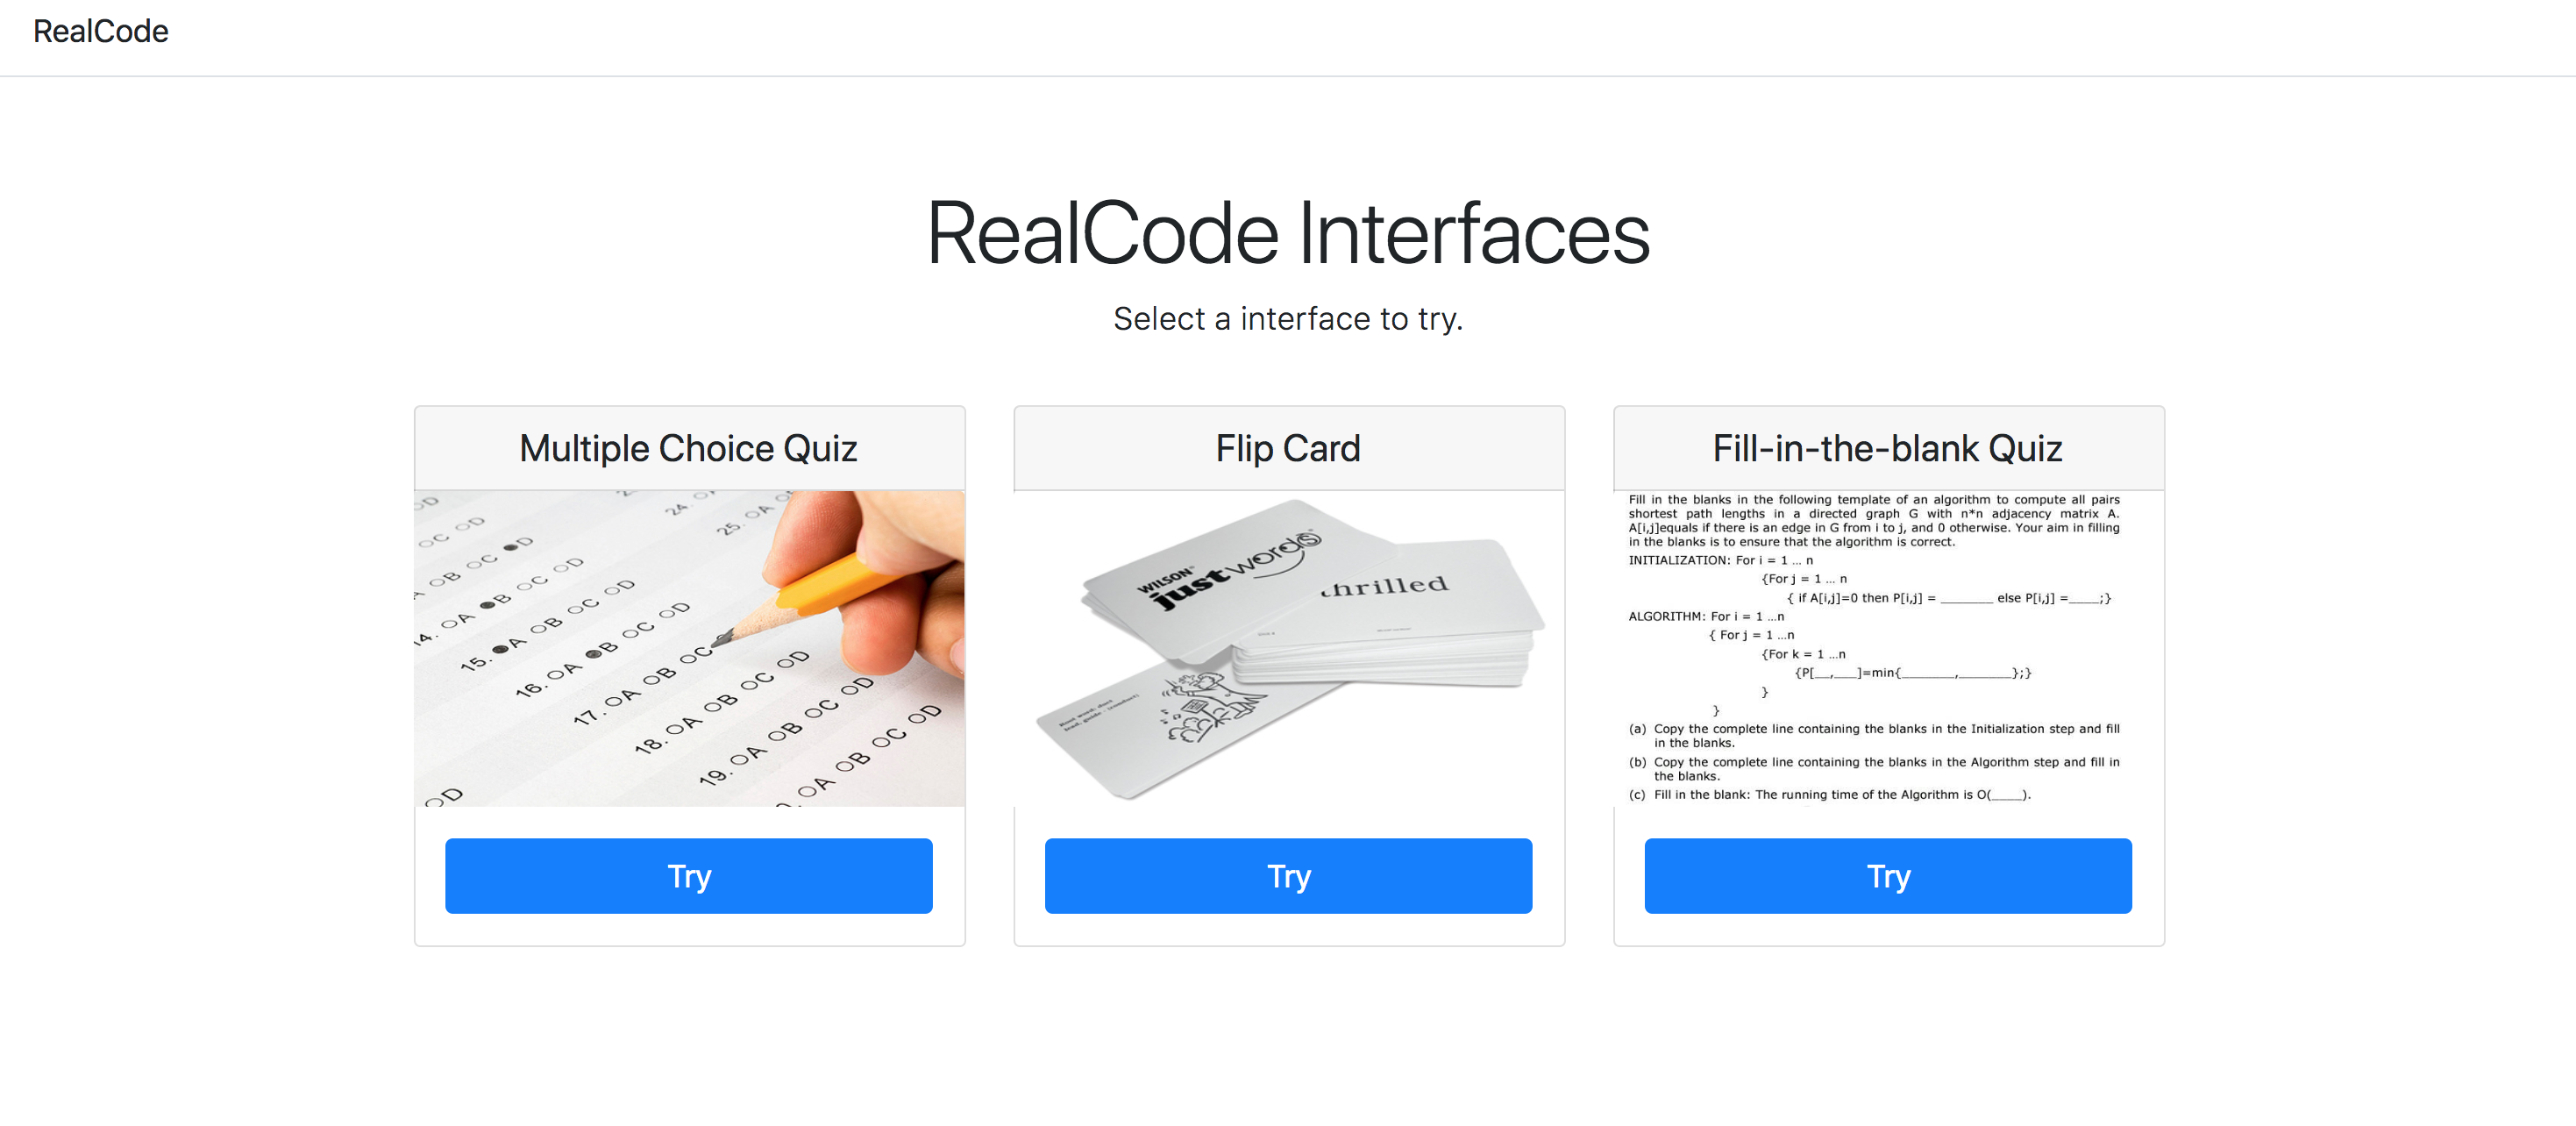
\includegraphics[width=1.0\columnwidth]{20181228-realcode-interfaces-select.png}
  \caption{デスクトップ版のRealCodeのインターフェース選択画面.}
  \label{fig:interface-selector}
\end{figure}

% \begin{figure}[H]
% 	\centering
%   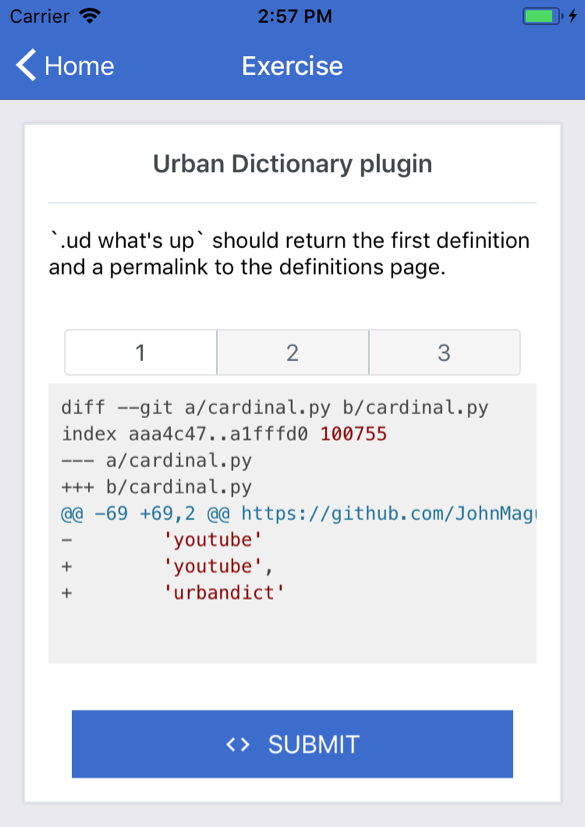
\includegraphics[width=1.0\columnwidth]{realcode_mobile.png}
%   \caption{モバイルのインターフェース.WIP.}
%   \label{fig:realcode-mobile}
% \end{figure}

\begin{figure}[H]
    \begin{tabular}{ccc}
      \begin{minipage}[t]{0.33\columnwidth}
        \centering
        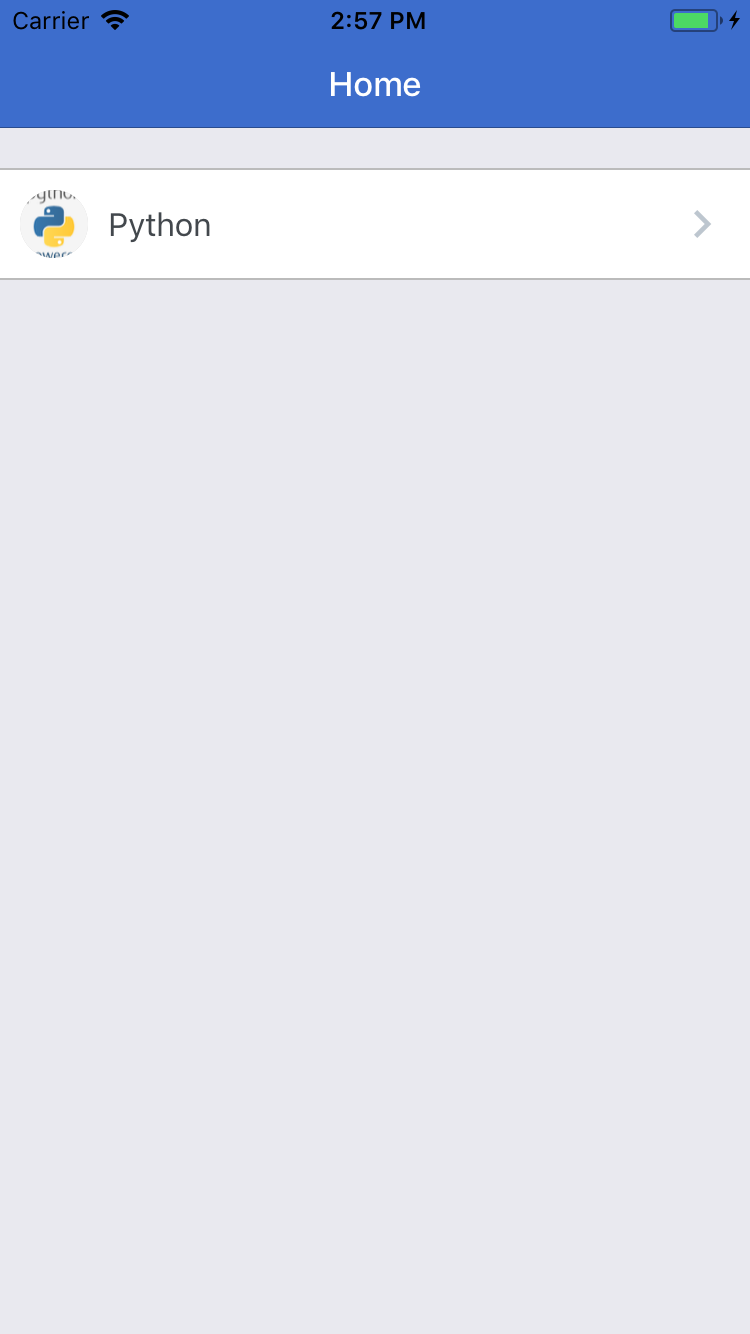
\includegraphics[width=1.0\columnwidth]{realcode-mobile-lang-selection.png}
        \subcaption{プログラミング言語の選択画面.}
      \end{minipage}
      \begin{minipage}[t]{0.33\columnwidth}
        \centering
        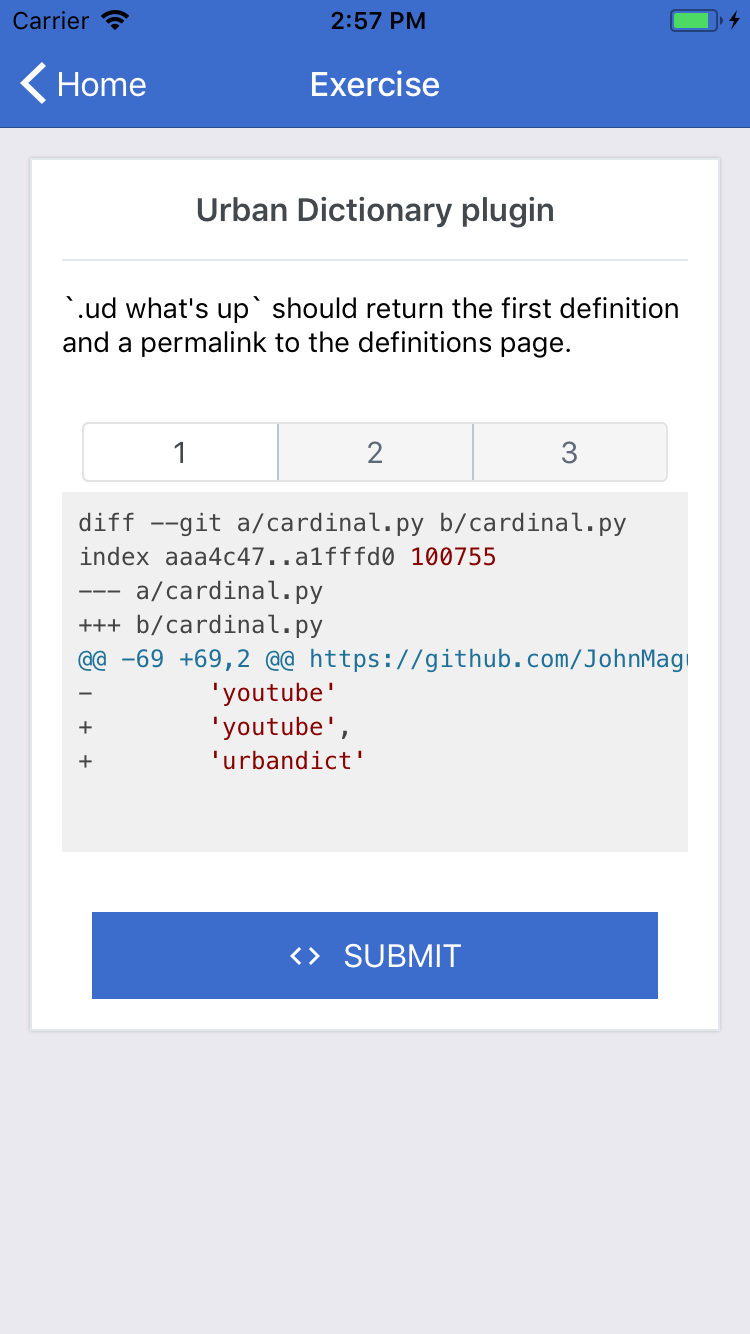
\includegraphics[width=1.0\columnwidth]{realcode-mobile-exercise.png}
        \subcaption{演習問題の画面.}
      \end{minipage}
      \begin{minipage}[t]{0.33\columnwidth}
        \centering
        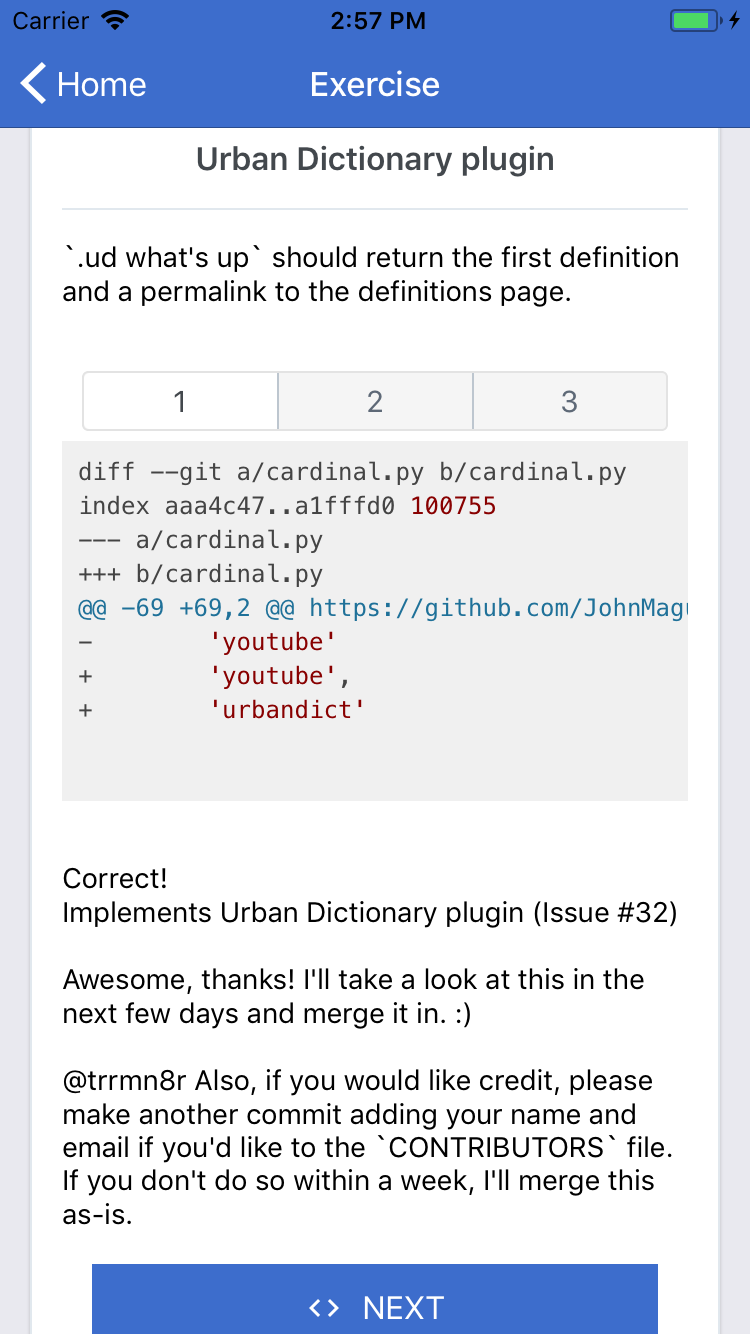
\includegraphics[width=1.0\columnwidth]{realcode-mobile-answer.png}
        \subcaption{演習問題の解答後の画面.}
      \end{minipage}
    \end{tabular}
    \caption{モバイル版のRealCodeのインターフェース.}
    \label{fig:realcode-mobile}
\end{figure}


\section{単語帳形式}

\begin{figure}[t]
    \begin{tabular}{cc}
      %---- Flip card, before ---------------------------
      \begin{minipage}[t]{1.0\columnwidth}
        \centering
        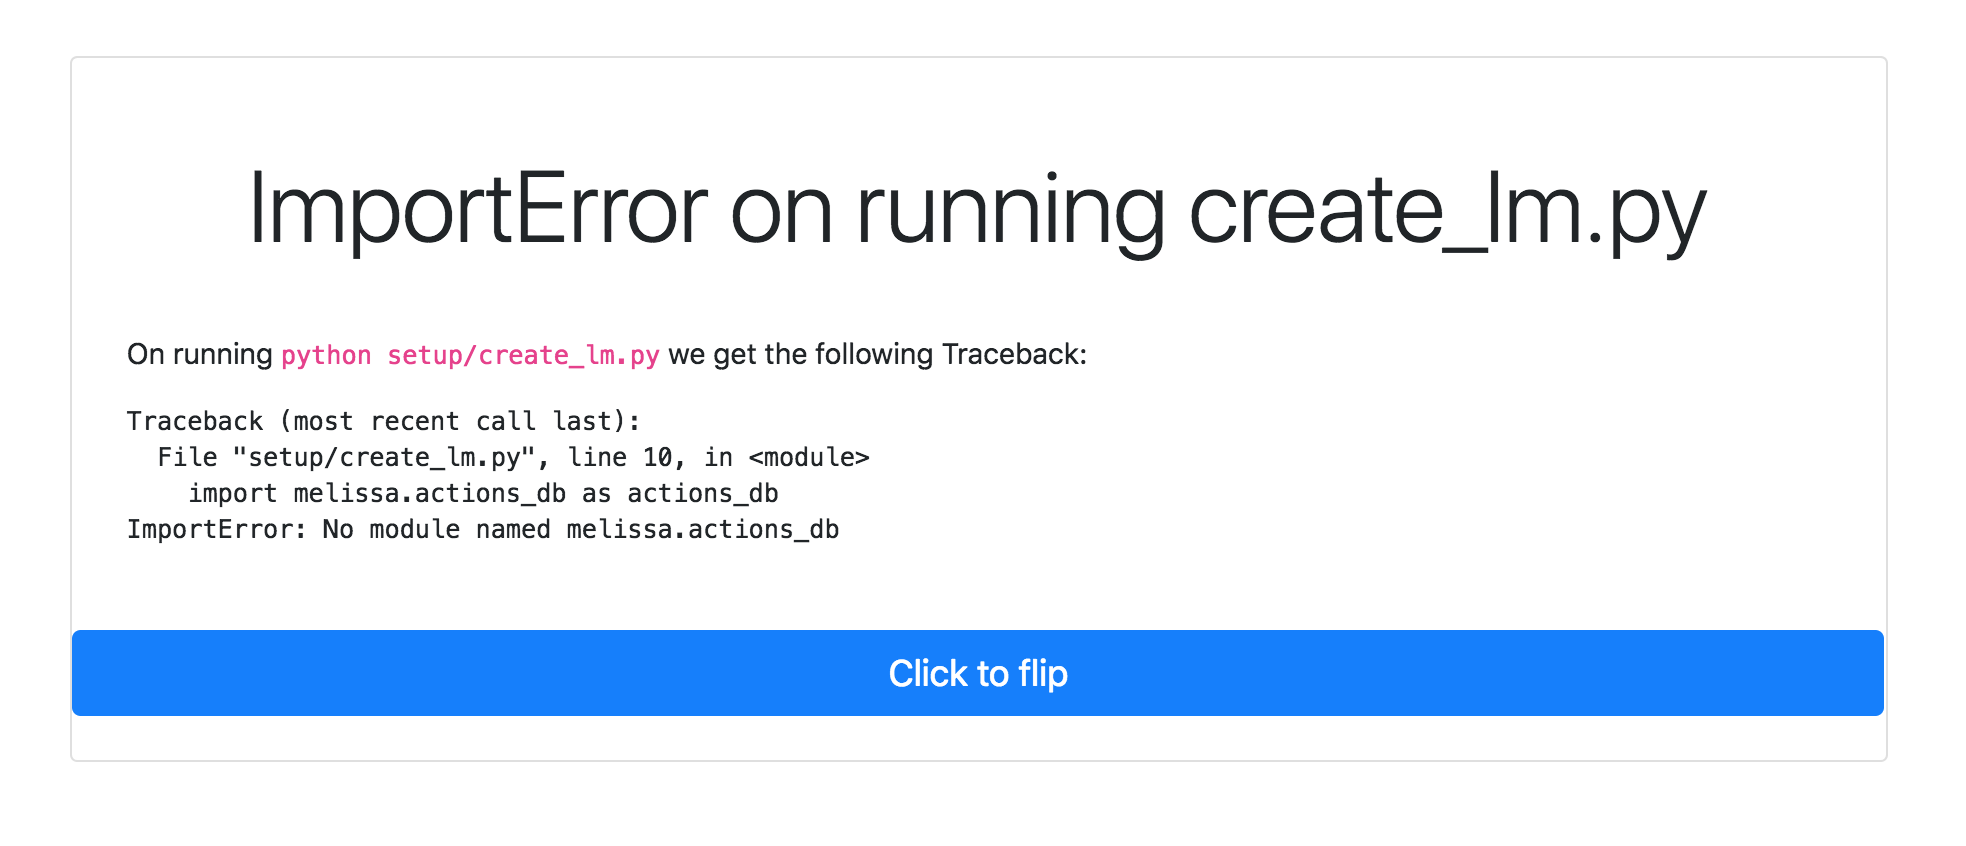
\includegraphics[width=1.0\columnwidth]{20181228-interface-flip-before.png}
        \subcaption{問題文側のインターフェース.}
        \label{fig:flash-before}
      \end{minipage} \\
      %---- Flip card, after --------------------------
      \begin{minipage}[t]{1.0\columnwidth}
        \centering
        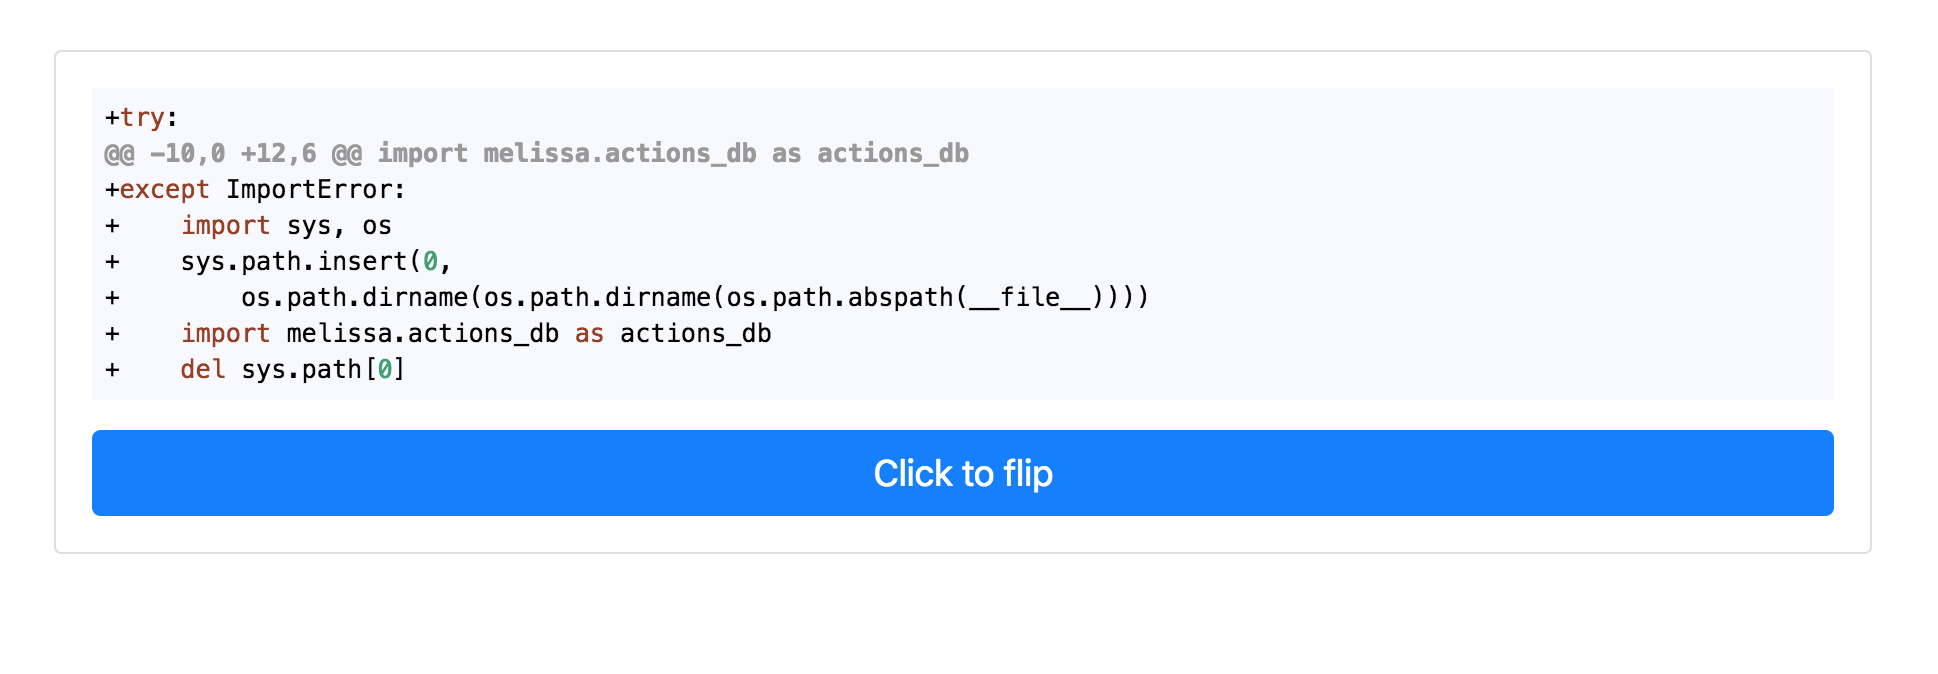
\includegraphics[width=1.0\columnwidth]{20181228-interface-flip-after.png}
        \subcaption{解答コード側のインターフェース.}
        \label{fig:flash-after}
      \end{minipage}
    \end{tabular}
    \caption{RealCodeの単語帳形式のインターフェース.``Click to flip''のボタンをクリックすることで,問題文と解答コードの画面を切り替えることができる.}
    \label{fig:flash}
\end{figure}

単語帳のようなフラッシュカードは繰り返し学習のための最も基本的な学習様式であり,特に反復による記憶に効果があることが確認されている~\cite{macquarrie2002comparison}.
図\ref{fig:flash}に示す単語帳形式のインターフェースを提供する目的は,問題文と解答コードを見比べて読むことにより,演習問題の鍵となる構文(例えば関数やAPIなど)の学習を促すことにある.
% 図\ref{fig:flash}に示すインターフェースにてユーザは問題文と解答コード見比べて読むことにより,演習問題の鍵となる構文(例,関数やAPIなど)を学習することを促す目的でこのインターフェースが提供されている.

% The \textit{FlashCard} interface is the most basic style for repeated learning~\cite{macquarrie2002comparison}.
% Users can simply review exercises and answer keys like flash cards.
% But unlike those for other purposes (e.g., vocabulary), it is not intended to make learners remember answer keys verbatim.
% Instead, learners are encouraged to examine what key components in the answer keys are (e.g., functions and APIs) and focus on remembering them.


\section{選択式}
\begin{figure}[t]
	\centering
  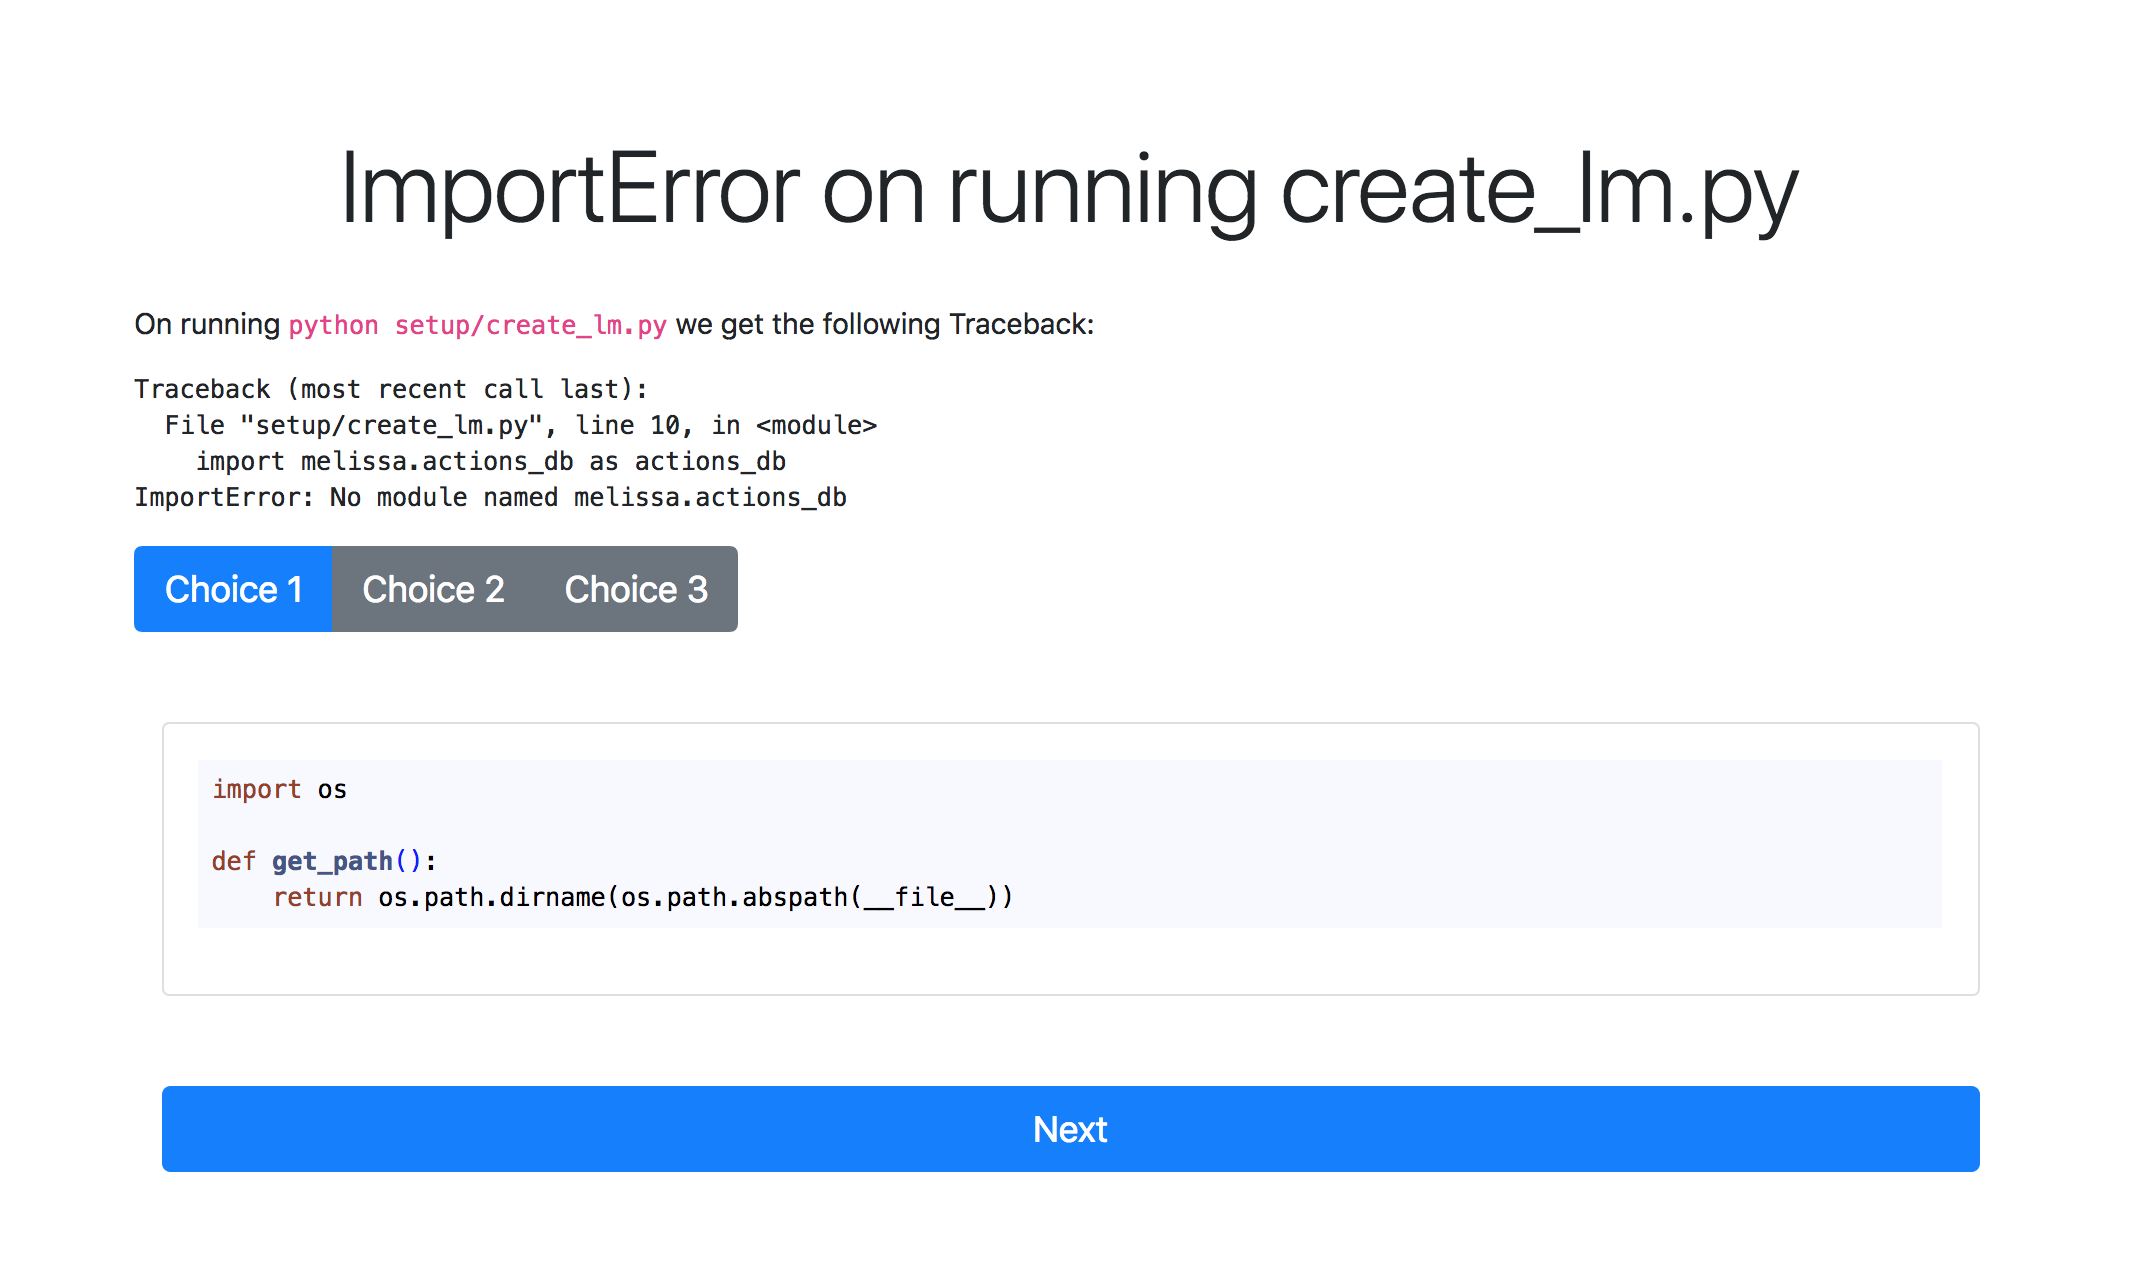
\includegraphics[width=1.0\columnwidth]{20181228-interface-mcq.png}
  \caption{RealCodeの選択式のインターフェース.``Choice~1'', ``Choice~2'', ``Choice~3''のボタンをクリックすると,解答の候補となる選択肢が表示される.}
  \label{fig:mcq}
\end{figure}

図\ref{fig:mcq}に示す選択式のインターフェースでは,演習問題ごとに解答の候補となる複数の選択肢(3択)を提供する.
適度な難易度の演習問題にするためには,不正解の選択肢は正解の選択肢の解答コードと似ていながらも異なっている必要がある.
例えばコメントのみが異なる(正解とすべき正しく動作する)コードを不正解の選択肢として提示した場合,選択式の問題としては不適切となる.
そこで各演習問題につき2つの適切な不正解の選択肢を生成するために,我々はプログラミング言語ごとにコードの文字列的類似度の上限値を定め,上限値を超えない中で最も類似度の高いコードを不正解の選択肢として提供することとした.
その上限値の設定方法は以下の通りである.
はじめに上限値を仮に1と設定する.
次に,ランダムに選択された50問の演習問題の解答コードに対して,その他の全ての演習問題の解答コードとの文字列的類似度をword-level fuzzy matching~\cite{sankoff1983time}により計算する.
そして,上限値を超えない中で最も類似度の高かった2つのコードが,解答コード例とどの程度異なるかを著者が判断した.
2つのコードが正解の選択肢と類似しすぎていた場合,上限値を0.05小さくしてから同様の処理を繰り返す.
以上の処理をプログラミング言語ごとに行うことで,上限値を決定している.
現在のプロトタイプでは上限値の決定を自動で行うことができないため,自動的に上限値が決定できるようになればRealCodeの拡張性がさらに高まると考える.



\begin{figure}[tb]
    \begin{tabular}{cc}
      %---- Flip card, before ---------------------------
      \begin{minipage}[t]{0.95\columnwidth}
        \centering
        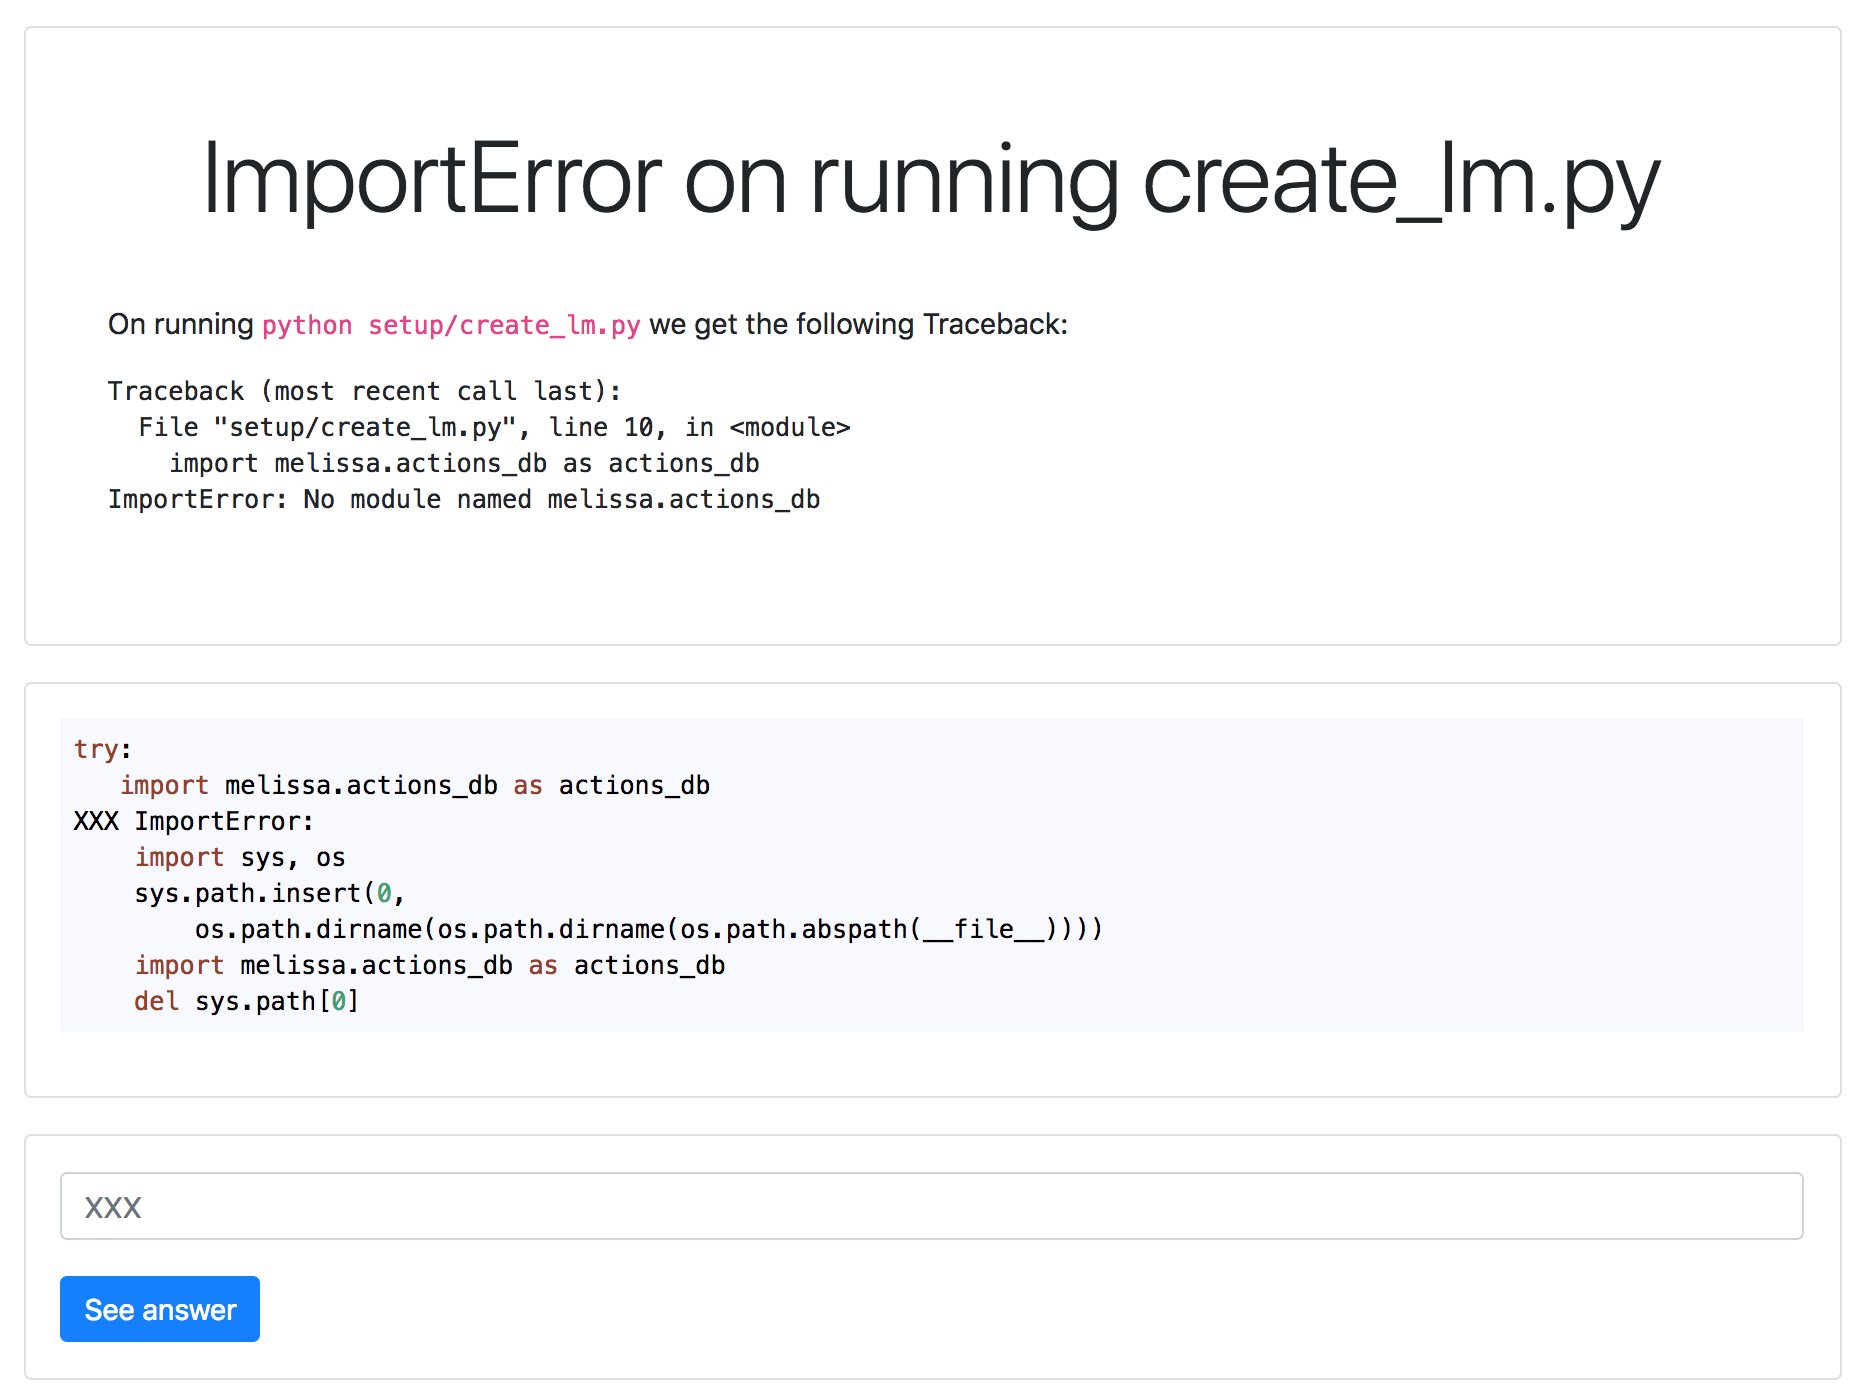
\includegraphics[width=0.9\columnwidth]{20181228-interface-fill-blank.png}
        \subcaption{回答前のインターフェース.ユーザは解答コード中の``XXX''に該当するPythonのコードを記述する.}
        \label{fig:fill-before}
      \end{minipage} \\ 
      %---- Flip card, after --------------------------
      \begin{minipage}[t]{0.95\columnwidth}
        \vspace{10 mm}
        \centering
        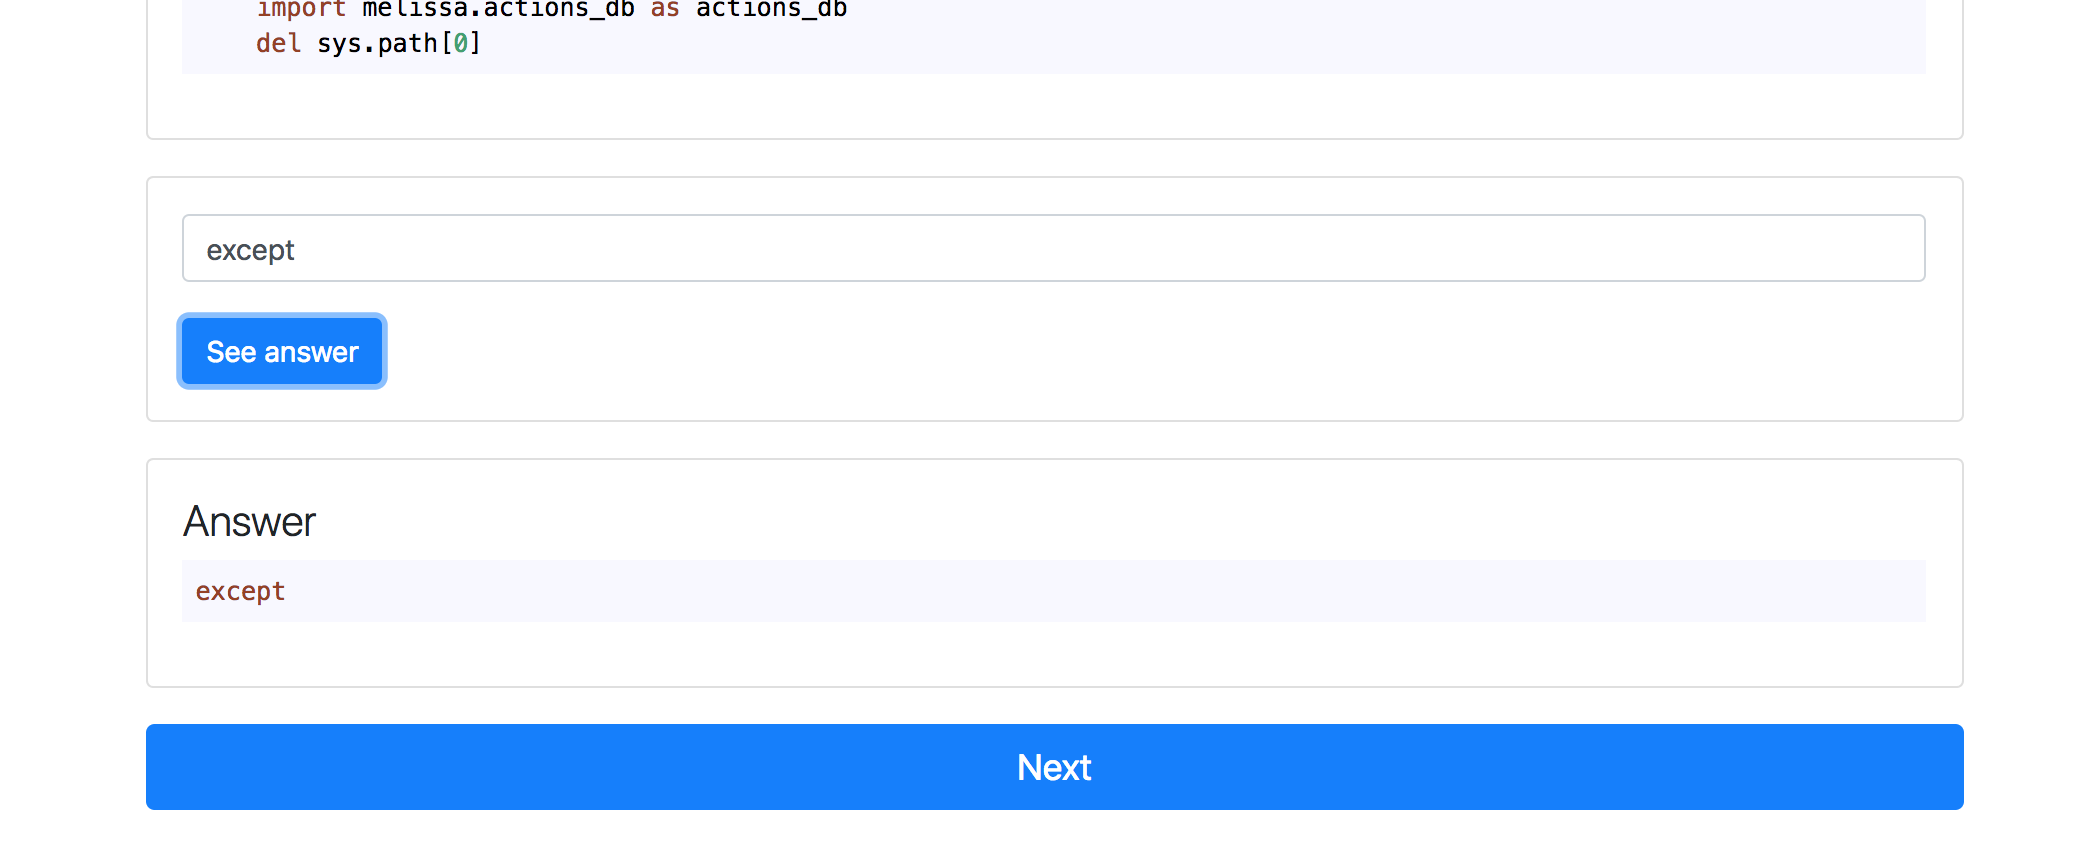
\includegraphics[width=1.0\columnwidth]{20181228-interface-fill-blank-after.png}
        \subcaption{回答後のインターフェース.}
        \label{fig:fill-after}
      \end{minipage}
    \end{tabular}
    \caption{RealCodeの穴埋め式のインターフェース.}
    \label{fig:fill}
\end{figure}

\section{穴埋め式}

図\ref{fig:fill}に示す穴埋め式のインターフェースでは,ユーザは問題文を読んだ後に解答コード中の空欄に該当するPythonのコードを記述する(例えば``for''や``except''など).
RealCodeはPythonで書かれた解答コードの構文木をあらかじめ作成し,その中からランダムに一か所を空欄とする.
現在のプロトタイプでは穴埋め式のインターフェースはPythonのみ対応しているが,構文解析を導入することで他のプログラミング言語にも対応することができる.
また,空欄とする構文をランダムでなくユーザが求める学習内容に応じて決定することができるようになれば,より体系的な学習体験を提供できるようになる可能性があると考える.

% The \textit{FillBlack} interface offers an advanced exercise by asking learners to fill a blank with a Python syntactic component (e.g., closures).
% Our system parses Python answer keys, and randomly selects one of components for a blank.
% Our current implementation supports this mode only in Python although extension to other languages is possible by integrating corresponding parsers.




%#
%# Evaluation chapters
%############################
%!TEX root = ../thesis.tex
%*******************************************************************************
%****************************** Fifth Chapter **********************************
%*******************************************************************************
\chapter{RealCodeが出題する演習問題の独自性評価}
\graphicspath{{Chapter5/Figs/}}


\label{section:ta_evaluation}


\ref{section:issue-classification}章にて述べたGitHubのイシューの抽出により,プログラミング演習問題に転用可能なイシューのデータセットを構築することができた.
しかし,教科書や授業で使用されている既存の演習問題とRealCodeが提供する演習問題がどう異なっているのかはまだ明らかになっていない.
そこで,大学でのプログラミングの講義においてティーチングアシスタント(TA)経験のある学生3名(PB1--PB3, 全て男性)によって,RealCodeが提供する演習問題の評価を行なった.
PB1とPB2は共に学部2年生を対象としたC言語の講義にて,TAとして授業中に様々な質問への回答や,テスト問題の作成を行なった経験がある.
PB3は学部3年生を対象とした別のC言語の講義において,C言語全般およびTCP/IPプロトコルについての質問対応と,最終レポートとプレゼンテーションの採点を担当していた.
% \ref{section:interview-study}章にてRealCodeのプログラミング演習問題を学生がどう感じるのかを理解するためのインタビューを行なった.
% その結果,GitHubに実在するイシューとプルリクエストを用いる事で実現されたRealCodeの長所を見つけ出す事が出来た.
% しかし,本研究の目的である実践的なプログラミング演習問題を提供できているのかは依然として明らかとなっていない.
% 特に,教科書や授業で使用されている既存の演習問題とRealCodeが具体的にどう異なっているのかを理解し,GitHub上に実在するデータを利用する事で提供可能となる新たな学習体験を明らかにする必要がある.


\section{実験方法}
現在のRealCodeのプロトタイプに存在する116件のPythonの演習問題に対し,実験参加者は以下の質問に5段階で評価を行った(1: 全く同意しない -- 5: 強く同意する).
また,評価の理由を自由記述の形式で述べることのできる項目を質問の最後に設けた.

\begin{itemize}
  \item[Q1.] 自分が担当した授業やそれ以外の授業・教科書で見たことのない・扱われている可能性がない内容か?
  \item[Q2.] 自分が担当した授業やそれ以外の授業・教科書と,この問題の違いは何か?
  \begin{itemize}
  	  \item Q2-1. 教科書で全く扱われていない範囲である
   	  \item Q2-2. 新しいAPIやライブラリの知識を必要とする
      \item Q2-3. あまり知られていないバグの修正を題材にしている
      \item Q2-4. 本番環境におけるバグの影響を実感できる
      \item Q2-5. ソフトウェアを本番稼働するための知識を必要とする
      \item Q2-6. チーム開発を意識したコードの書き方
  \end{itemize}
\end{itemize}

\subsection{実験結果}

\begin{table}[t]

  \centering
  \caption{TAによるシステム評価実験のQ2に関する,授業で扱われていないと判断された課題数.(表中の``agreed''は,「授業で扱われていないと判断された」を意味する. また,母数はQ1に対し3人中2人以上が「同意する」または「強く同意する」と回答し,かつ残りの一人が「全く同意しない」以外を回答した75問の演習問題である.)
%   (\masaki{母数}{「母数」って言い方合ってましたっけ..}はQ1に対し3人中2人以上が「同意する」または「強く同意する」と回答し,かつ残りの一人が「全く同意しない」以外を回答した75問の演習問題)\sakaguchi{}{表の中の「agree」が文中で述べられていないのであれ?となってしまいました…加えて,「結果」でもいいのですが,できれば「授業で扱われていないと判断された課題数」など具体的にあると嬉しいです}
}
  \label{table:ta_evaluation_result}
    
  \begin{tabular}{l | c c} \Hline
  
  & \# of agreed & 率[\%] \\ \hline \hline
  Q2-1(教科書の範囲外) & 50 & 66.67 \\
  Q2-2(新しいAPIやライブラリ) & 40 & 53.33 \\
  Q2-3(知られていないバグの修正) & 35 & 46.67 \\
  Q2-4(バグの影響の実感) & 55 & 73.33 \\
  Q2-5(実際のシステムに必要な知識) & 49 & 65.33 \\
  Q2-6(チーム開発の実感) & 20 & 26.67 \\  \Hline
  \end{tabular}
\end{table}

Q1に関して,3人中2人以上が「同意する」または「強く同意する」と回答し,かつ残りの一人が「全く同意しない」以外を回答した演習問題を,「授業・教科書では扱われていない課題」とみなすこととした.
これは半数以上の同意が得られたと同時に,強い反対がなかった演習問題を抽出するためである.
評価の結果,116問中75問(63.6\%)が授業・教科書では扱われていない課題と判断されたことがわかった.
その75問において,Q2の各選択肢に対してQ1と同様に,3人中2人以上が「同意する」または「強く同意する」と回答し,かつ残りの一人が「全く同意しない」以外を回答した演習問題の数を表\ref{table:ta_evaluation_result}に示す.

\subsection*{本番環境におけるバグの影響の体験}

本実験の結果,Q2-4(本番環境におけるバグの影響を実感できる)が最も同意を得られた項目であった.
RealCodeでは,実際のソフトウェアにおいて発生したバグを修正するイシューを転用した演習問題が多く提供されているからであると考えられる.
例えば,異なるOSで実行した際に発生するエラーを修正する演習問題において,RealCodeが実践的なバグ修正方法に関する知識を提供可能であることが示唆された.

\myquote{windowsとlinuxの違いを意識させられるし,OSの違いをうまく吸収するコーディングを学べる}{PB1}

また,実際のソフトウェア開発で頻発する問題の現実的な解決方法をRealCodeの演習問題が提供していることも確認された.

\myquote{不安定なコネクションという課題に対して実際に用いられている対策を学ぶことができる}{PB3}

\myquote{「この実行方法はサポートされていない」ということを明示的に出す経験は教科書や授業では扱わないと感じた}{PB1}


\subsection*{既存の学習環境で扱われていない内容の学習}

Q2-1(教科書で全く扱われていない範囲)はQ2-4に次いで同意が得られた項目であった.
例えばソフトウェアのテストを書くことは,既存の授業や教科書ではあまり扱われていない.
しかし,実際のソフトウェア開発においてテストは品質を保証する上で推奨される慣習である.
RealCodeではソフトウェアのテストに関する演習問題も提供されていることが確認された.

\myquote{授業でテストやテスティングライブラリを扱うことはあまりない}{PB2}

\myquote{テストを書くのは,既存のコードに合わせて書く必要があるので,その場で考える実践的な訓練になりそう}{PB1}

実際のソフトウェア開発では,ユーザにとって使いやすいシステムを実装することが求められる.
しかし,既存の教育素材においてシステムの利便性の向上を目指すといった正解のない演習問題はあまり見られない.
PB1の次のコメントは,RealCodeがシステムの使いやすさを向上するための知見を提供できることを示唆している.

\myquote{アルゴリズムの勉強というより,使いやすくするためにどうすればよいか?ということを考えさせられる部分が,授業や教科書では得られない体験}{PB1}




\subsection*{ソフトウェアの本番稼働に関する知識の習得}

また,Q2-5(ソフトウェアを本番稼働するための知識を必要とする)は,Q2-1に次いで同意が得られた項目であった.
ソフトウェアを安定的に本番稼働させるためには,コード変更を本番環境に反映させたり,本番環境のサーバの状況を監視したりする必要がある.
しかし,本番稼働に関する知見が教科書に記載されていることは少なく,RealCodeが既存の学習環境とは異なる視点から知見を提供できる可能性がある.

\myquote{continuous integrationができるように修正する経験は,授業や教科書ではあまりできない}{PB3}




























%!TEX root = ../thesis.tex
%*******************************************************************************
%****************************** 6th Chapter **********************************
%*******************************************************************************
\chapter{RealCodeが出題する演習問題の学習者視点から主観的評価}
\graphicspath{{Chapter6/Figs/}}

\label{section:interview-study}

\ref{section:ta_evaluation}章にて述べたRealCodeが出題する演習問題のTA経験者による独自性評価により,GitHubのイシューを転用することで実現された演習問題の特徴を明らかにすることができた.
続いて我々は,学習者がRealCodeの演習問題をどう感じるのか理解するために,プログラミングの講義の受講経験とPythonの使用経験を持つ8人の大学生(PC1--PC8, 全て男性)にインタビューを行った.
RealCodeのインターフェースの簡単な説明の後に,実験参加者に自由にRealCodeを操作してもらった.
実験参加者の主観的な印象に先入観を与えないため,RealCodeがどのようにプログラミング演習問題を生成しているのかの説明は意図的に省略した.
そして,実験の最後にRealCodeに対する印象や感想について約20分のインタビューを行った.


% \ref{section:issue-classification}章にて述べたイシューの分類により,プログラミング演習問題として活用出来ると考えられるデータセットを構築することができた.
% しかしRealCodeが提供する演習問題のユーザ・エクスペリエンスはまだ明らかとなっていない.
% そこで我々はユーザがRealCodeの演習問題をどう感じるのか理解するために,ソフトウェアの講義の受講経験がありかつPythonの使用経験がある8人の大学生(PC1--PC8, 全て男性)にインタビューを行った.
% 簡単なRealCodeのインターフェースの説明の後に,実験参加者に自由にRealCodeを操作してもらった.
% 実験参加者の主観的な印象に先入観を与えないために,我々はRealCodeがどのようにプログラミング演習問題を生成しているのかを意図的に説明しなかった.
% そして,実験の最後にRealCodeに対する印象や感想について約20分のインタビューを行った.
% 本章ではインタビューの結果について述べる.

% %Our quantitative examination on selection heuristics revealed a potential to extract appropriate issues and code diffs for exercise creation.
% %However, the user experience of programming exercises generated by RealCode is still unknown.
% We next conducted an informal qualitative study to understand how learners perceive exercises in our system.
% We recruited eight university students (PC1--PC8, all male) who had taken at least one software course and had Python programming skills.
% After we explained our interfaces, participants were asked to freely explore the system.
% We deliberately provided no explanation about how our system generated exercises to avoid potential biases in their subjective impressions.
% Our post-experimental interviews were conducted to examine how our participants described RealCode exercises.
% %We offered approximately 10 USD in local currency as a compensation. % 1000 yen.

% We transcribed the interviews and performed open-ended coding to categorize quotes.
% We faithfully translated quotes as faithfully as possible for report because our interviews were conducted in a local language.

\section*{開発にて実際に発生したバグ・トラブルの体験}
RealCodeの最も特徴的な要素は,プログラミング演習問題をGitHub上に実在するイシューおよびプルリクエストから生成していることにある.
例えばバグ修正は実践的なソフトウェア開発における一般的な作業であるが,一般的なプログラミング演習問題ではあまり扱われていない.
PC2とPC3はバグ修正に関するRealCodeの演習問題が彼らにとって新鮮な体験であると述べた.

% The most unique aspect of exercises in RealCode is that they are based on actual issues and code diffs.
% Bug fixes are a common activity in real-world software development, but existing programming exercises do not cover in general.
% PC2 and PC3 were excited when they saw a bug fix exercise because it is not what they would normally see in textbooks.
% Such exercises also encouraged our participants to consider what they would need to learn as PC1 commented.

% P2: トラブルシューティングみたいな問題は見たことないから,結構面白いかも

% P3: あんまりこういうエラーが発生してそれにどう対処すべきか,みたいな問題を経験したことがないから,なんか新鮮で面白そう.
\myquote{トラブルシューティングみたいな問題は見たことないから,結構面白いかも.}{PC2}

\myquote{あんまりこういうエラーが発生してそれにどう対処すべきか,みたいな問題を経験したことがないから,なんか新鮮で面白そう.}{PC3}
% \myquote{I have never tried exercises on how to solve an error code. It is eye-opening and intriguing to me.}{PC3}

PC1は,このようなバグ修正の演習問題は実践的な知識の学習意欲を向上させる可能性があると述べており,これはRealCodeが提供する演習問題の1つの利点であると考えられる.


% P1: 開発における問題点の解決のためのプログラミング知識を意識させられるなあと感じた
\myquote{(RealCodeの演習問題は)開発における問題点の解決のためのプログラミング知識を意識させられるなあと感じた.}{PC1}
% \myquote{[Exercises in our system] made me think of what programming knowledge I would need to solve problems in real development.}{PC1}

PC6はRealCodeの演習問題はソフトウェア開発の授業においてより適当であるという感想を述べている.
これもRealCodeが教科書等とは違った演習問題を提供できていることを示唆するコメントである.

% PC6 ultimately summarized the characteristics of exercises in RealCode by emphasizing that they would fit to development-oriented learning.

% P6: 普通の授業で使うのは少し違う気がする.授業で扱うべきは基礎だと思うし.ただ,プロジェクト型の授業とか,学ぼうというより開発系の授業なら全然いいと思う.
\myquote{普通の授業で使うのは少し違う気がする.授業で扱うべきは基礎だと思うし.ただ,プロジェクト型の授業とか,学ぼうというより開発系の授業なら全然いいと思う.}{PC6}
% \myquote{I feel [RealCode] would not work in normal classes. They should teach basics. But if you are in project-based or development-oriented classes, [RealCode] would be really good.}{PC6}

\section*{プログラミング知識の実践的な活用方法の体験}

実験参加者は講義や教科書を通じてPythonを学んだ経験があるが,Pythonの実践的な開発経験は必ずしもなく,RealCodeでの演習問題を通して,Pythonの様々な利用法を見ることが可能となっていた.

% Our participants had learning experience of Python through courses and textbooks.
% But they did not necessarily experience different applications of the language due to lack of development opportunities.
% Two participants (PC2 and PC8) commented their excitement of discovering new Python use.

% P2: (問題をみて)へーPythonってこんな低レイヤーなことできるんですね
\myquote{(問題をみて)へーPythonってこんな低レイヤーなことできるんですね.}{PC2}
% \myquote{(Seeing one exercise,) I did not know that Python can do this low-level thing.}{PC2}

% P8: 今までやったPythonって文法とデータ分析くらいで,web周りに使ってるのは初めて見たし面白い
\myquote{今までやったPythonって文法とデータ分析くらいで,web周りに使ってるのは初めて見たし面白い.}{PC8}
% \myquote{I've learned Python only about the syntax and for data analysis. This is my first time to see Python for Web development, and it makes the exercises interesting.}{PC8}

上記のような例は実際のソフトウェア開発はよく見られる可能性があるものの,教科書等では記載されていることが少なく,RealCodeが既存の教育素材とは違った視点で,演習問題を提供できていることを示す1つの例である.

また,RealCodeの演習問題は問題文に開発目的や背景知識を含んでいるものが多い.
そういった情報は開発の動機を説明しており,演習問題が実践的なソフトウェア開発を想定していることを実験参加者に実感させることも可能となっていた.

% Similarly, exercises on RealCode often contain background stories and explanations of development objectives.
% They explain motivations for revising code, and improve the perceived practicality of exercises on RealCode.

% P4: 開発の背景というか現状把握に時間がかかるけど,話にストーリーがあって面白い.(~ would be great, というセリフを見て)何かのサービスを改善したい,から問題が始まってるのは,学習のモチベーション的にいい.
\myquote{開発の背景というか現状把握に時間がかかるけど,話にストーリーがあって面白い.(``would be great'' という一文を見て)何かのサービスを改善したい,から問題が始まってるのは,学習のモチベーション的にいい.}{PC4}

% \myquote{It takes time to understand the background of an exercise. But such a story makes the exercise interesting. This problem has a story like a person wants to improve a service. That's a good motivation for learning too.}{PC4}


\section*{開発チームにおけるコミュニケーションの体験}


ソースコードの可読性はチーム開発における開発速度やソフトウェアの質そのものに大きく寄与するが,可読性に重点をおいているプログラミング演習問題は少ない.
一方,RealCodeは実際のコード変更を演習問題に転用しているため,可読性の高いコードやコード中のコメントを含んでいることが実験参加者によって指摘されていた.
そのような解答コード例は学習者の可読性に対する意識を高めることができる可能性があり,RealCodeはコードの書き方に関する教育的効果をもたらす可能性が示唆された.

% Source code readability is critical for quality control as well smooth communication among developers.
% But existing exercises do not typically emphasize readability.
% PC2 and PC5 noticed that answer keys on RealCode often contain readable code and many comments.
% These answer keys can contribute to increasing learner's awareness of code readability.

%P2: なんかコードが形式ばってないですね,わりと可読性を意識して書かれてる気がします.

% P5: コード内にコメントがたくさんあって,なんとなくこう可読性というか人に見られることを意識していていいね.
\myquote{コード内にコメントがたくさんあって,なんとなくこう可読性というか人に見られることを意識していていいね.}{PC5}

% \myquote{Answer code includes many comments. Looks like the code is intended to be seen by others, and that's good.}{PC5}


また,PC8はソフトウェア開発におけるコミュニケーション特有の用語や略語が多く含まれている事を指摘した.
実際の開発ログから演習問題を生成する事で開発特有の表現が含まれるようになるため,実践的な開発の一部を垣間見ることができることが示唆されている.

% Participants also noticed slangs and abbreviations that are commonly used in communication among developers. 
% Exercises in textbooks do not contain such terms, and our participants felt more reality by seeing them.

\myquote{英語というか,実践的な表現が学べて面白い.開発特有の表現とか.LGTMとかエラーの表現とか今まで知る機会がなかった.}{PC8}

% \myquote{It is interesting to see expressions exercises use. I did not have an opportunity to know ``LGTM (looks good to me)'' or other error-related expressions until now.}{PC8}



% Comparison to programming classes
% P1: 講義は教養的な知識が多すぎる
% P6: 授業の方がもっと根本からプログラミングを学べるけど,少しハイレイヤーというか俯瞰的に学ぶための問題としてなら結構いいと思う






\section*{各インターフェースの特徴}

8人の実験参加者のうち,7人が選択式のインターフェースが最も良いと述べた.
選択式のインターフェースでは解答方法が簡単であるため,プログラミング学習を始めたばかりの学習者に適していると考えられる.

% Seven of the participants preferred \textit{MultiChoice} the most.
% They agreed that \textit{MultiChoice} offered a good starting point for learning as answering does not necessarily require proficient knowledge.

% P1: 1番目(MCQ)は気軽に取り組みやすそう.特に俺みたいな授業でPythonやっただけの人には答えやすい
\myquote{(選択式のインターフェース)は気軽に取り組みやすそう.特に俺みたいな授業でPythonやっただけの人には答えやすい}{PC1}
% \myquote{\textit{MultiChoice} looks a good entry point to me. Especially for those who learned Python only in a class like me, it is easy to answer.}{PC1}


% Fill
3人の実験参加者ら(PC5,PC6,PC8)は,穴埋め式のインターフェースではPythonの文法を詳しく学ぶことができると指摘した.
一方でPC2は,穴埋め式のインターフェースではPythonの文法のごく一部のみが扱われるため,選択式のインターフェースの方が学習に適していると述べた.
これらのことから,学習者が学習したい内容に合わせて,インターフェースが使い分けされることが想定される.
% Three interviewees (PC5, PC6, and PC8) also liked \textit{FillBlank} because they can learn details on Python syntax.
% However, PC2 pointed out that \textit{MultiChoice} is better because requires learners to examine the whole code changes instead of only a part of it.
% P2: 穴埋めだと一つの構文の勉強だけになっちゃうから,構文は結構わかるし,全体的に読む(MCQ)問題形式の方がいい
\myquote{穴埋めだと一つの構文の勉強だけになっちゃうから,構文は結構わかるし,全体的に読む問題形式(選択式)の方がいい}{PC2}
% \myquote{The fill-in-the-blank is more for studying one particular syntax rule. But I already know syntax well, so \textit{MultiChoice} is better for me because I need to read all lines [of code changes].}{PC2}




% Flip
他のインターフェースと異なり,単語帳形式のインターフェースは実験参加者らから不評であった.
特にプログラミング初心者にとって,イシューの説明文から解答となるコードを推測することは難易度が高すぎることが示唆されていた.

% Unlike the other interfaces, \textit{FlashCard} was not popular in our study.
% PC7 stated that it is too difficult for non-experts to give any similar code to the answer key.
% P7: この解答どうりに答えれることは無いし,答え合わせがしづらくて嫌かも.上級者にはいいのかもしれないが,僕には少し難しすぎるかもしれない
\myquote{この解答どうりに答えれることは無いし,答え合わせがしづらくて嫌かも.上級者にはいいのかもしれないが,僕には少し難しすぎるかもしれない.}{PC7}
% \myquote{It is impossible to give the exact same answer to the answer code. Also hard to check if I am correct. Maybe good for advanced learners, but a little too difficult to me.}{PC7}



% \subsection*{Areas for Improvements}
% Although the interviewees found benefits of \XXX, they also pointed out several limitations.
% P4, P6 and P7 stated that it is hard to understand contexts of exercises on \XXX.
% % P4: 何を問うているのかが少し分かりにくいかなあ,ただこれがそういう面の理解も含めての演習ならすごくいいと思う
% % P6: 前提知識が少し多い気がする,何を聞かれているのかが分かるまでに時間がかかる.
% % P7: 色々役立つtipsみたいなのが散らばってていいと思うが,何を聞かれているのかが少し分かりにくいと感じた.

% \myquote{Many advance knowledges are required. Difficult to understand what the exercise says.}{PA6}




% \newpage

% \subsection{Experiment Design}

% \subsubsection{Task}

% Dataset:
% \begin{itemize}
%   \item Quizzes created from the \XXX system
%   \item Quizzes created from Sanfoundry
% \end{itemize}

% Test:
% \begin{itemize}
%   \item 3 Tests (Test A, B, and C)
%   \item Each test has 20 Python quizzes created from the \XXX system.
% \end{itemize}

% Task:
% \begin{itemize}
%   \item Both groups first take Test A.
%   \item First learning for 3 days. (Group A: Quiz-GitHub, Group B: Quiz-Sanfoundry). Notice that participants have to answer more than 50 quizzes.
%   \item Both groups then take Test B.
%   \item Second learning for 3days (Group A: Quiz-Sanfoundry, Group B: Quiz-GitHub). Notice that participants have to answer more than 50 quizzes.
%   \item Both groups take Test C.
% \end{itemize}

% Compensation:
% \begin{itemize}
% 	\item 5,000 yen and additional rewards according to a number of answered quizzes
% \end{itemize}


% \subsubsection{Participants}

% We set the following criteria for participants: 1) they must be junior or senior; 2) they must have taken at least one computer science course; 3) they had not joined software development.
% Our participants thus would be students who have learned programming in a course but do not have joined software development in a real world.
% We recruited 10 students for our evaluation (\shibato{}{P1--10; 9 male and 1 female}).


% \subsubsection{Procedure}

% Our participants first were asked to come to our laboratory for this study.
% After they signed a consent form, we explained the \XXX system and tasks, and gave time for practice.
% The participants then took \textit{Test 1}.


% \subsection{Results}

% \subsubsection{3 Tests}
% We conducted multi-level linear regression analysis to quantitatively examine the contribution of \XXX.


% \subsubsection{Questionnaire}


% \subsubsection{Time and Location}


% \subsubsection{Final Questionnaire}
% TBD


















%#
%# Lab study
%# https://github.com/IIS-Lab/ShibatoM/wiki/Analysis-of-lab-study をまとめる.
%############################

\chapter{RealCodeが出題する演習問題の分類評価}
\label{section:lab-study}
\graphicspath{{Chapters_evaluation/Figs/}}


\ref{section:ta_evaluation},\ref{section:interview-study}章にて述べたRealCodeの評価実験により,イシューをプログラミング演習問題へと転用することで,既存の学習環境にはない独自の演習問題を提供できることが明らかとなった.
しかし,RealCodeの演習問題からどのような内容(例えば文法やアルゴリズム)を学習できるのかは明らかとなっていない.
そこで,RealCodeの演習問題から学習可能な内容を理解するために,著者によるRealCodeの演習問題の分類評価を行った.


\section{実験方法}

現在のRealCodeのプロトタイプに存在する116件のPythonの演習問題に対し,図\ref{fig:lab-study}に示す分類評価用のインターフェースから,著者は以下の質問に回答した.

\begin{itemize}
  \item[Q1.] This is a good exercise to you. (1: Disagree -- 3: Agree)
  \item[Q2.] What did you learn from this exercise?
  \begin{itemize}
  	  \item 文法
   	  \item アルゴリズム
      \item ライブラリやAPIの使い方
      \item 自分が経験した・見たことのあるバグの解決方法
      \item ソフトウェアのテスト
      \item デザイン
      \item ウェブ
      \item データベース
      \item 例外処理
      \item メンテナンス
      \item その他学んだこと(記述式)
  \end{itemize}
\end{itemize}

\begin{figure}[H]
 \centering
  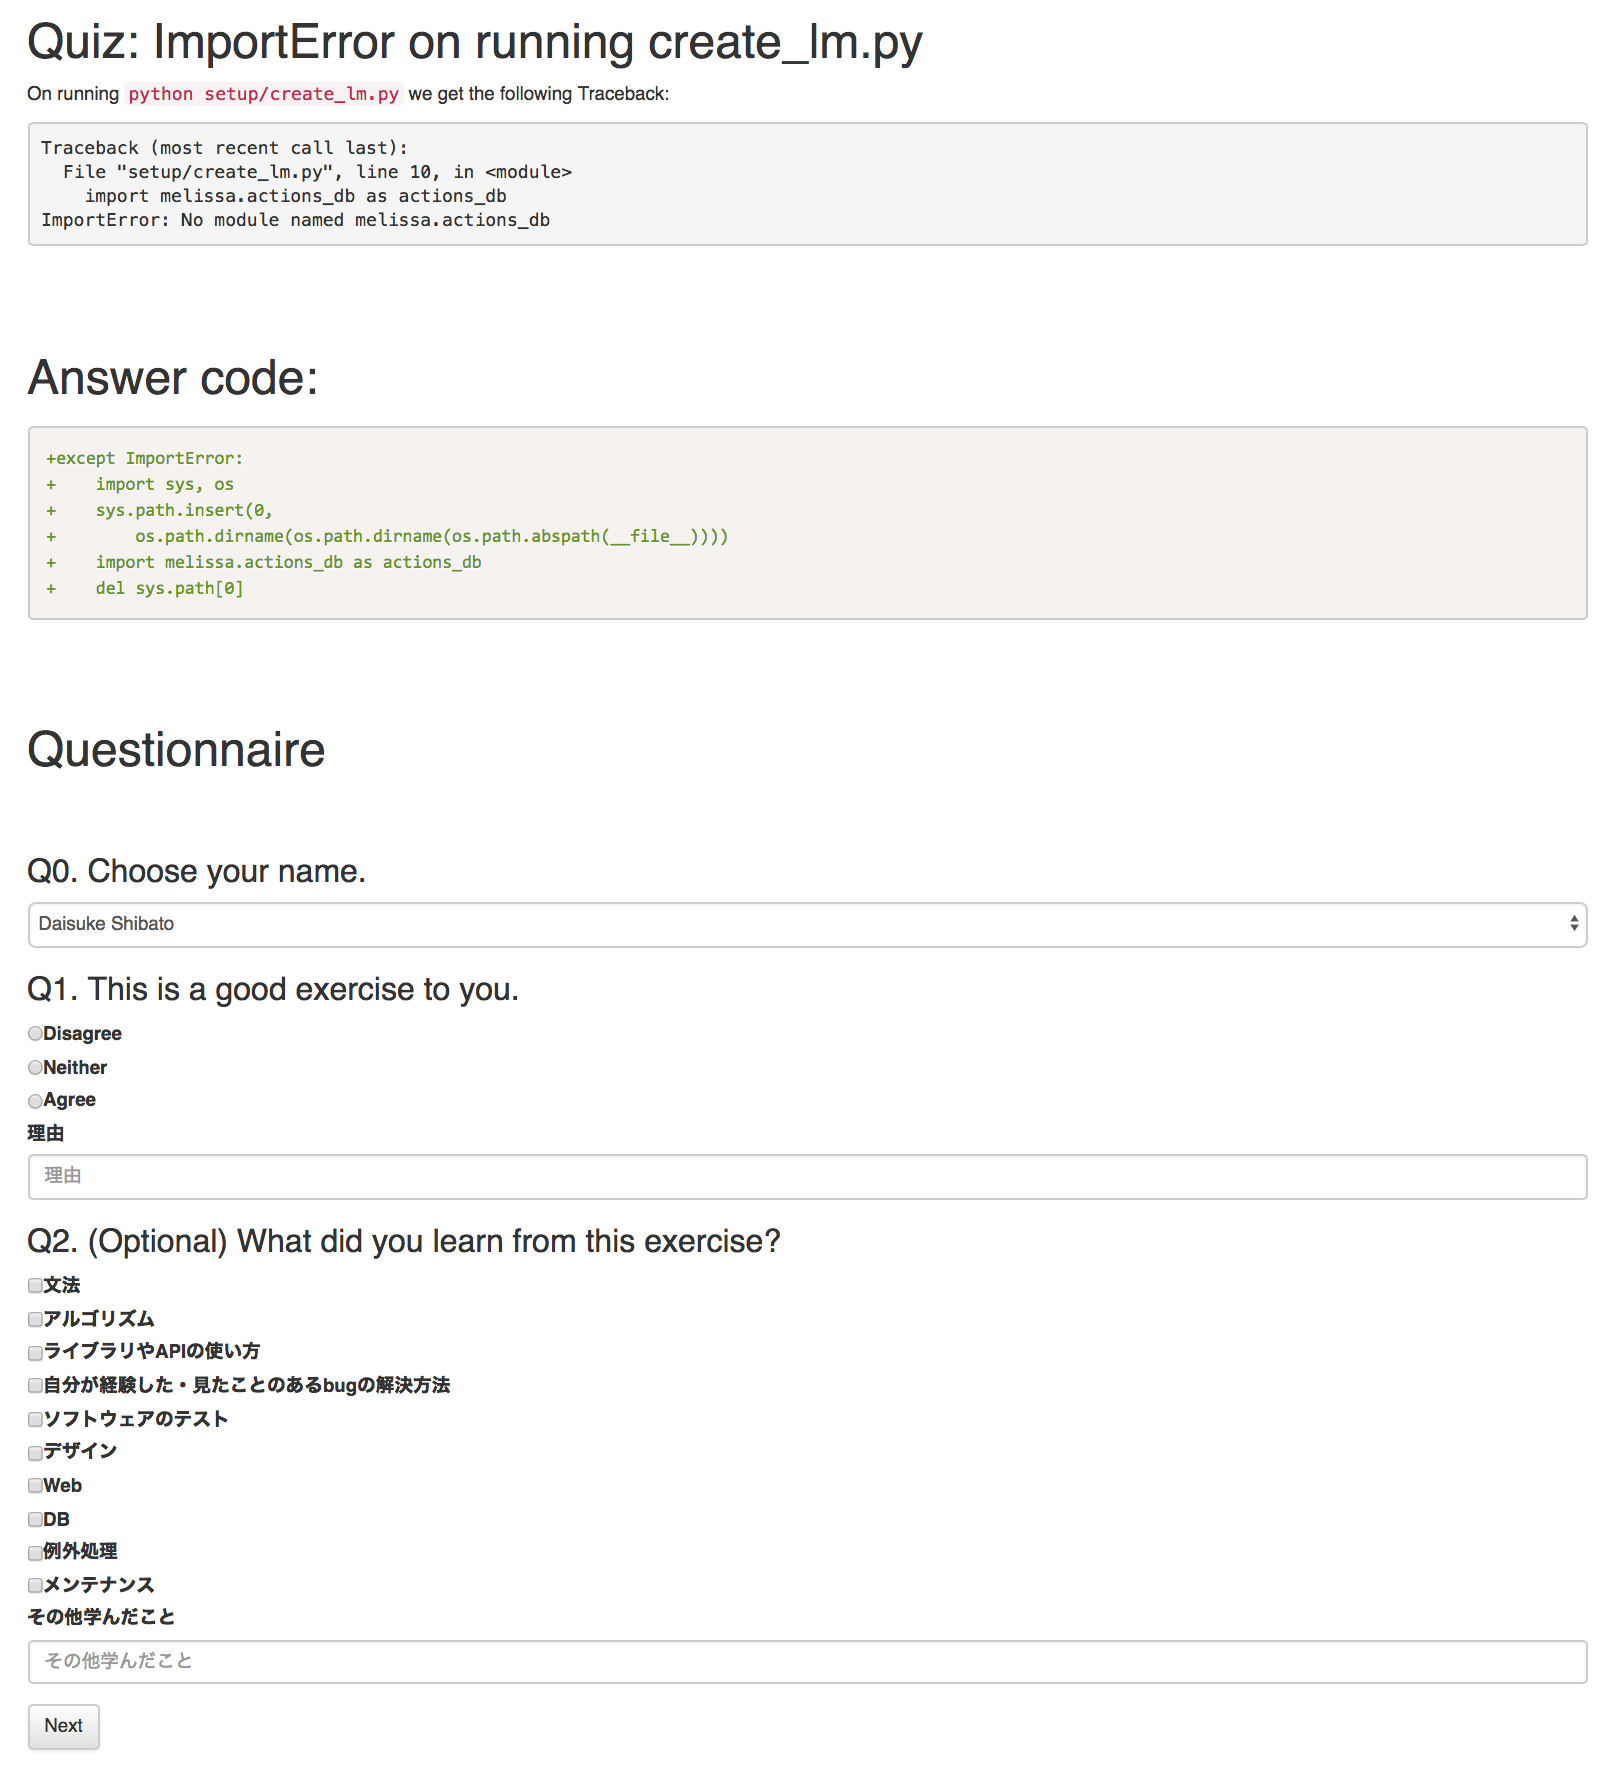
\includegraphics[width=1.0\columnwidth]{20181218-lab-study-interface-all.png}
  \caption{RealCodeが出題する演習問題の分類評価にて用いたインターフェース.}
  \label{fig:lab-study}
\end{figure}

\section{実験結果と考察}

\begin{table}[b]
  \centering
  \caption{RealCodeが出題する演習問題の分類評価におけるQ2の結果.但し,母数はQ1に対し``Agree''と回答された48問の演習問題である.}
  \label{table:lab-study-q2-result}
  \begin{tabular}{ l | c } \Xhline{3\arrayrulewidth}
      分類 & 割合(\%) \\ \hline \hline
      例外処理 & 12.85 \\
      メンテナンス & 12.29  \\
      自分が経験した・見たことのあるバグの解決方法 & 9.50 \\
      ライブラリやAPIの使い方 & 6.70 \\
      アルゴリズム & 2.79 \\
      Web & 2.79 \\
      文法 & 1.12 \\  
      デザイン & 0.56 \\
      DB & 0.56 \\
      \Xhline{3\arrayrulewidth}
  \end{tabular}
\end{table}

Q1に対して,41.4\%の演習問題が``Agree'',18.1\%が``Neither'',40.5\%が``Disagree''として回答した.
また``Disagree''の理由として,1)コード変更がわかりづらい,2)リファクタリングのみが行われている,3)著書が知らなかったライブラリのAPIが多く使用されている,の3つの要因が多く挙げられた.

回答結果を確認した結果,コード変更がわかりづらい要因として,コード変更量が数行程度といった断片的なものであることや,既存の関数の一部の変更といった局所的なものであることが明らかとなった.
また,使用されている変数の多くがコード変更の外で宣言されている場合も,コード変更がわかりづらいと判断した.
これらのような演習問題をデータセットから除外する手法の一つとして,演習問題のコード変更と全体のソースコードの構文解析を行い,外部変数の使用割合や文法的コード変更の分類を特徴量として決定木に与えることが考えられる.
しかし,現在のRealCodeのプロトタイプは様々なプログラミング言語に対応するために意図的に構文解析を導入していない.
RealCodeの演習問題において頻繁に使用されているプログラミング言語の構文解析を実装することで,RealCode上の演習問題数を保ちながら,コード変更がわかりづらい演習問題を除外できると考える.

また,リファクタリングのみが行われている演習問題からはプログラミングに関する知識を得ることができないと判断した.
なぜなら,リファクタリングのコード変更は変数名やインデントの変更などのみから構成されているためである.
コード変更がリファクタリングであるかどうかを判定するためには,構文解析を使用した手法と,コード変更の繰り返しを検出する手法が考えられる.
構文解析を用いてコード変更が構造的に変更されているかどうかを判定することで,一般的に構造的には変更しないリファクタリングを検出できると考えられる.
また,コード変更内に繰り返し発生する変更パターンを検出できた場合も,リファクタリングであると判断できる.
後者は構文解析を用いることなく実装できるため,様々なプログラミング言語に対応しながら実装することができる可能性がある.

また,著者が知らなかったライブラリのAPIが多く使用されている演習問題では,そもそもコード変更を理解することができなかったため``Disagree''と回答した.
このような演習問題の多くが,デバッグツールやコンソールアプリといった,著者にとってあまり馴染みのないリポジトリから生成されていた.
ユーザのプログラミング経験や知識に応じて,演習問題の生成元であるリポジトリをあらかじめ選定できるようになれば,ユーザが知らないライブラリが多く使用された演習問題を除外できる可能性がある.

次に,Q2の回答結果を表\ref{table:lab-study-q2-result}に示す.
特に回答の割合の高かった例外処理,メンテナンス,自分が経験した・見たことのあるバグの解決方法,ライブラリやAPIの使い方の4つの分類について考察を行う.


\subsection{例外処理に関する演習問題}

例外処理に関して学ぶことができるとラベル付けされた演習問題には,文字コードのエンコードエラーやネットワークの接続エラーが発生した際の対応策に関するものが多く含まれていた.
例えば図\ref{fig:lab-study-eg-exception}に示す演習問題では,Pythonのtry,catch構文を用いて``Unicode Encode Error''という例外に対応している.
ソフトウェアを本番稼働させるためには,起こりうる例外を想定しあらかじめ対策しておくことが重要であるが,一般的なプログラミング演習問題ではあまり扱われていない~\cite{Piteira_Learning_Computer_Programming}.
RealCodeの例外処理に関する演習問題を通じて,ソフトウェアを本番稼働させた際に発生しうる例外とその対応策に関する知識を習得できる可能性がある.

\begin{figure}[H]
  \centering
  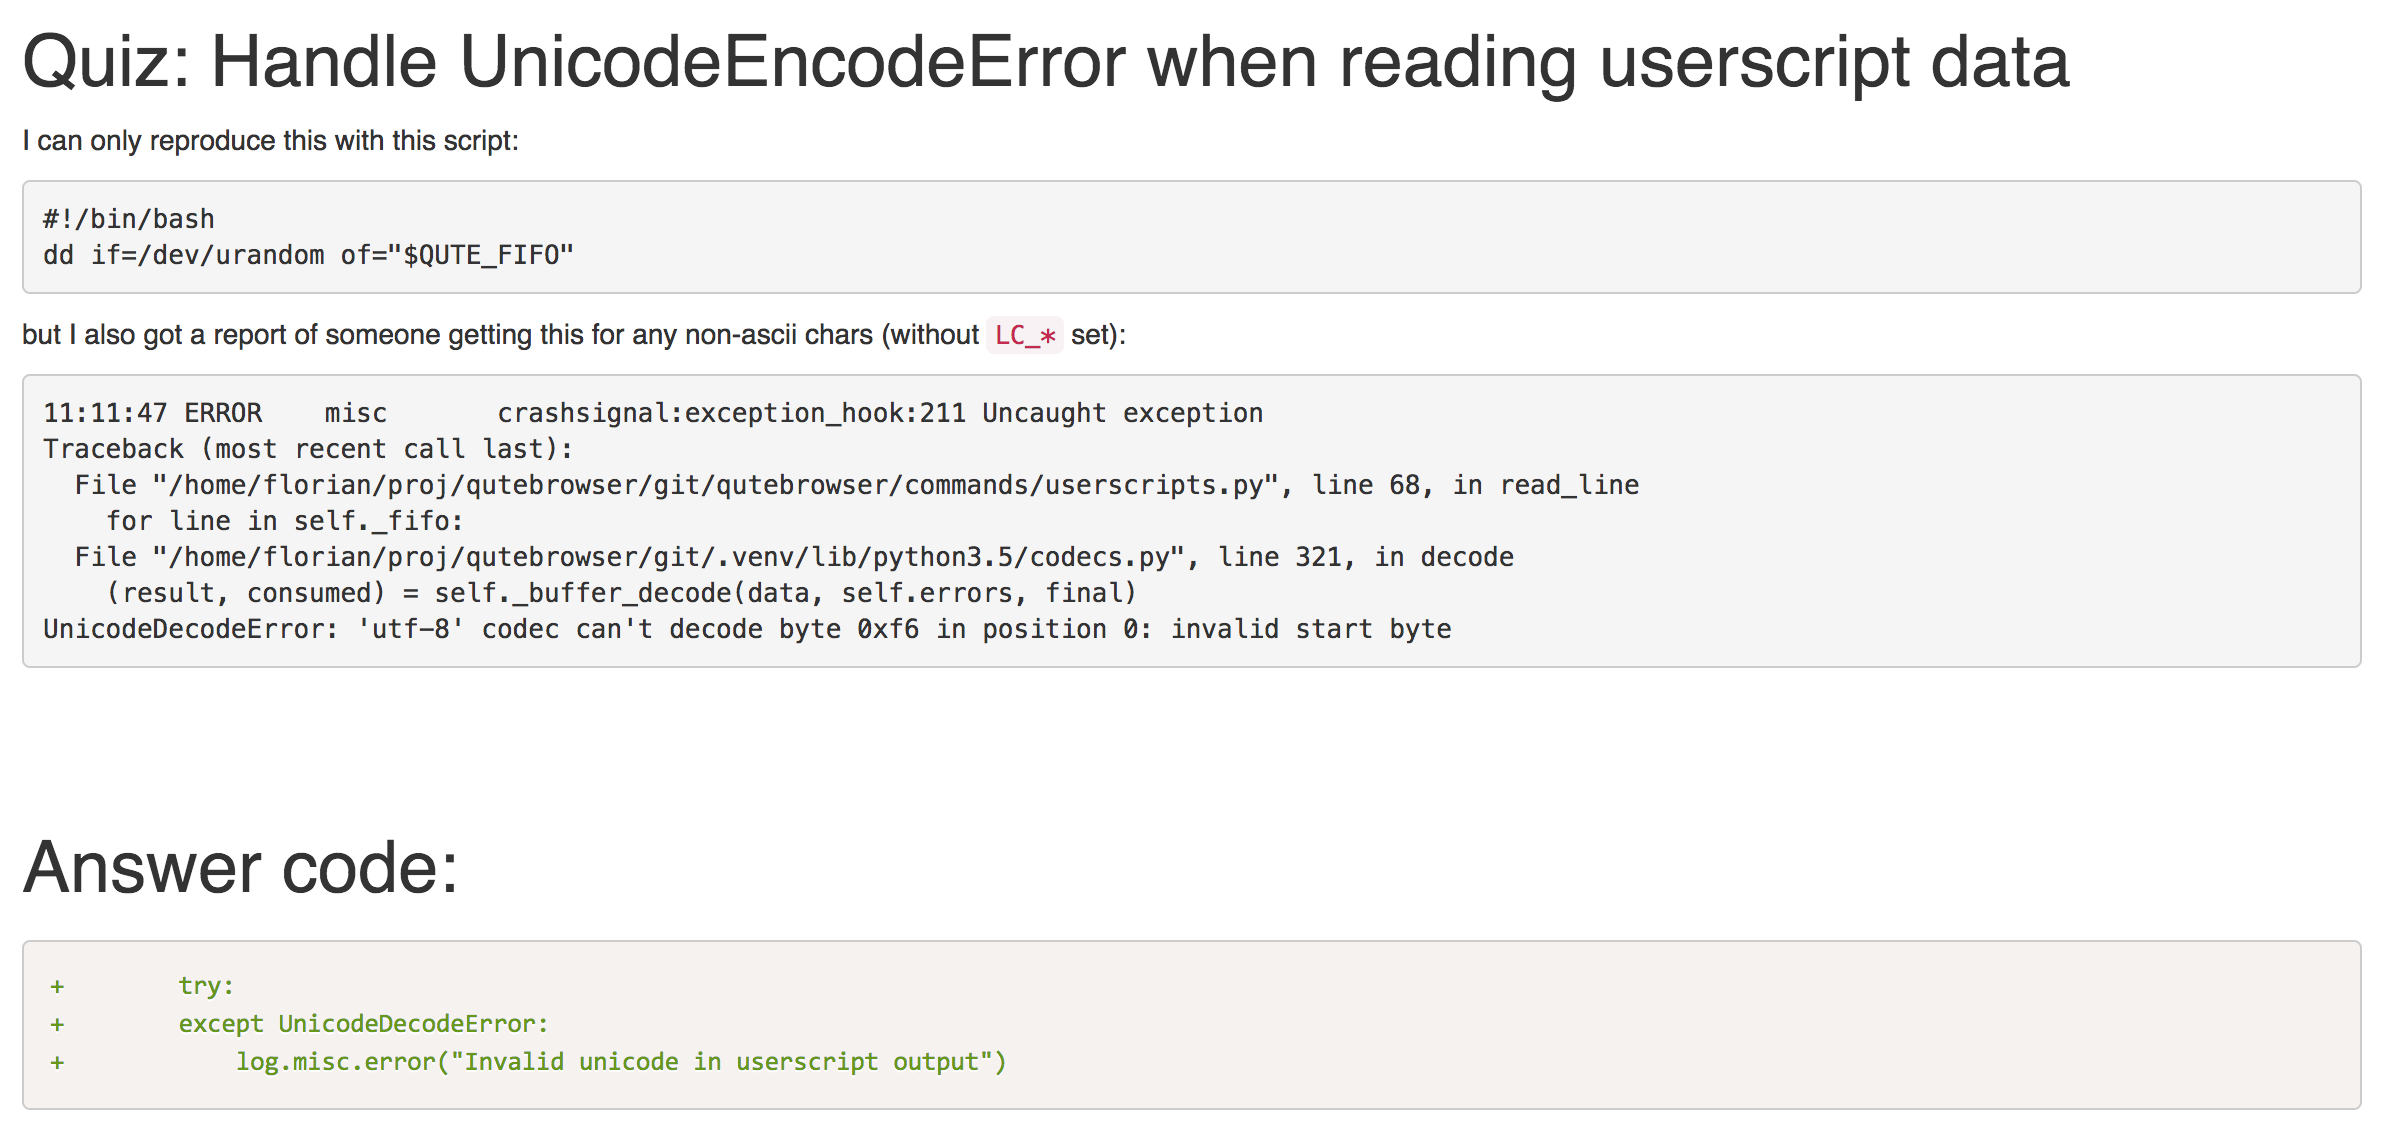
\includegraphics[width=1.0\columnwidth]{20190107-lab-study-exception-exercise2.png}
  \caption{例外処理に関する演習問題の例.``Unicode Encode Error''の例外に対して,Pythonのtry,catch構文を用いて対応している.}
  \label{fig:lab-study-eg-exception}
\end{figure}


\subsection{メンテナンスに関する演習問題}

本番稼働中のソフトウェアにて障害が発生した際に迅速に対応するためには,動作中のソフトウェアのログを取得しておくことが重要である~\cite{kernighan1999practice}.
図\ref{fig:lab-study-eg-maintenance}に示す演習問題の例では,動作しているソフトウェアのプロセス番号をログに追加するコード変更を行なっている.
プロセス番号があらかじめ分かっていれば,ソフトウェアの動作状況を監視できると同時に,障害発生時にも速やかな対応を行うことが可能となる.
RealCodeのメンテナンスに関する演習問題から,ソフトウェアの実装だけでなく,運用していく上での知識も学習できる可能性がある.

\begin{figure}[H]
\vspace{-0.05cm}
	\centering
  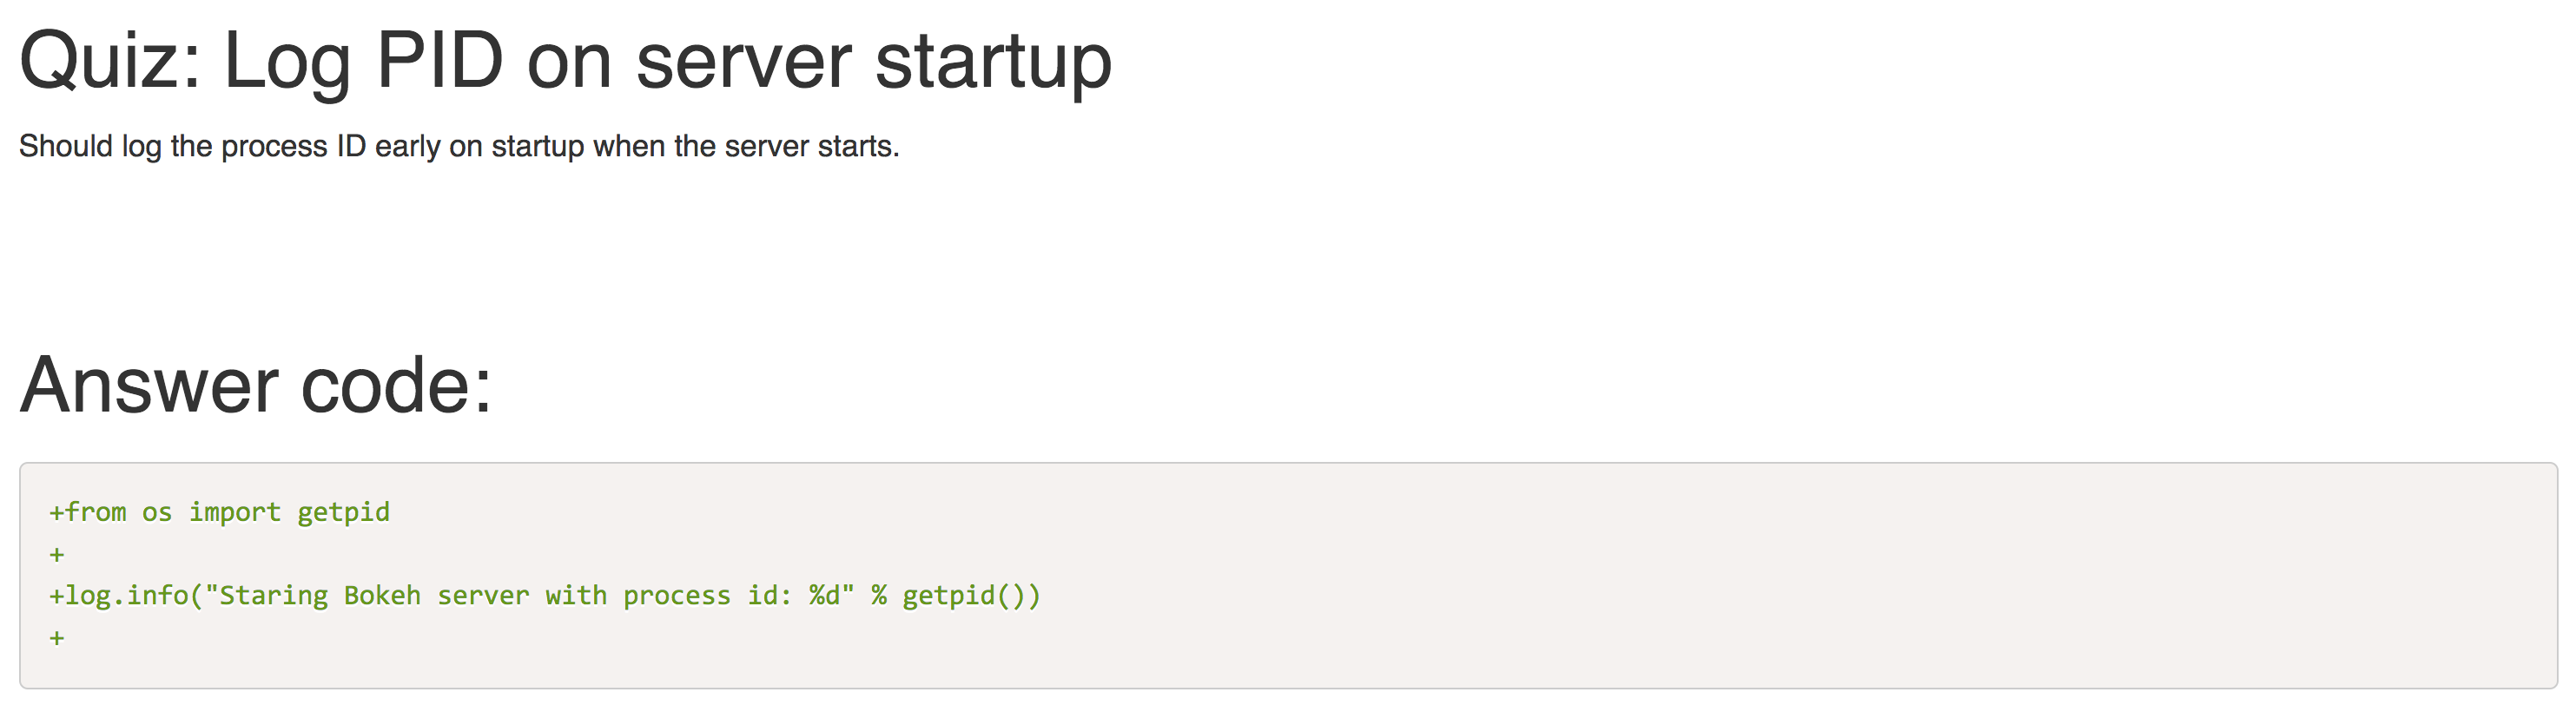
\includegraphics[width=0.95\columnwidth]{20190107-lab-study-maintenance-exercise.png}
  \vspace{-0.05cm}
  \caption{ソフトウェアのメンテナンスに関する演習問題の例.起動時にプロセス番号をログに出力している.}
  \label{fig:lab-study-eg-maintenance}
  \vspace{-0.35cm}
\end{figure}

\subsection{自分が経験した・見たことのあるバグの解決方法に関する演習問題}

RealCodeの演習問題はGitHubに実在するイシューとプルリクエストから生成されており,頻発するバグに関する演習問題が多く含まれている.
図\ref{fig:lab-study-eg-experience}に示す演習問題では,データベースの名前にピリオドは使用できないという,データベースを扱う際に頻発するバグを取り扱っている.
このようなプログラミングの基礎知識ではないが実装する上でよく発生する問題は一般的なプログラミング学習材料では扱われておらず,RealCode特有の演習問題であると言える.

\begin{figure}[H]
 \centering
 \vspace{-0.3cm}
 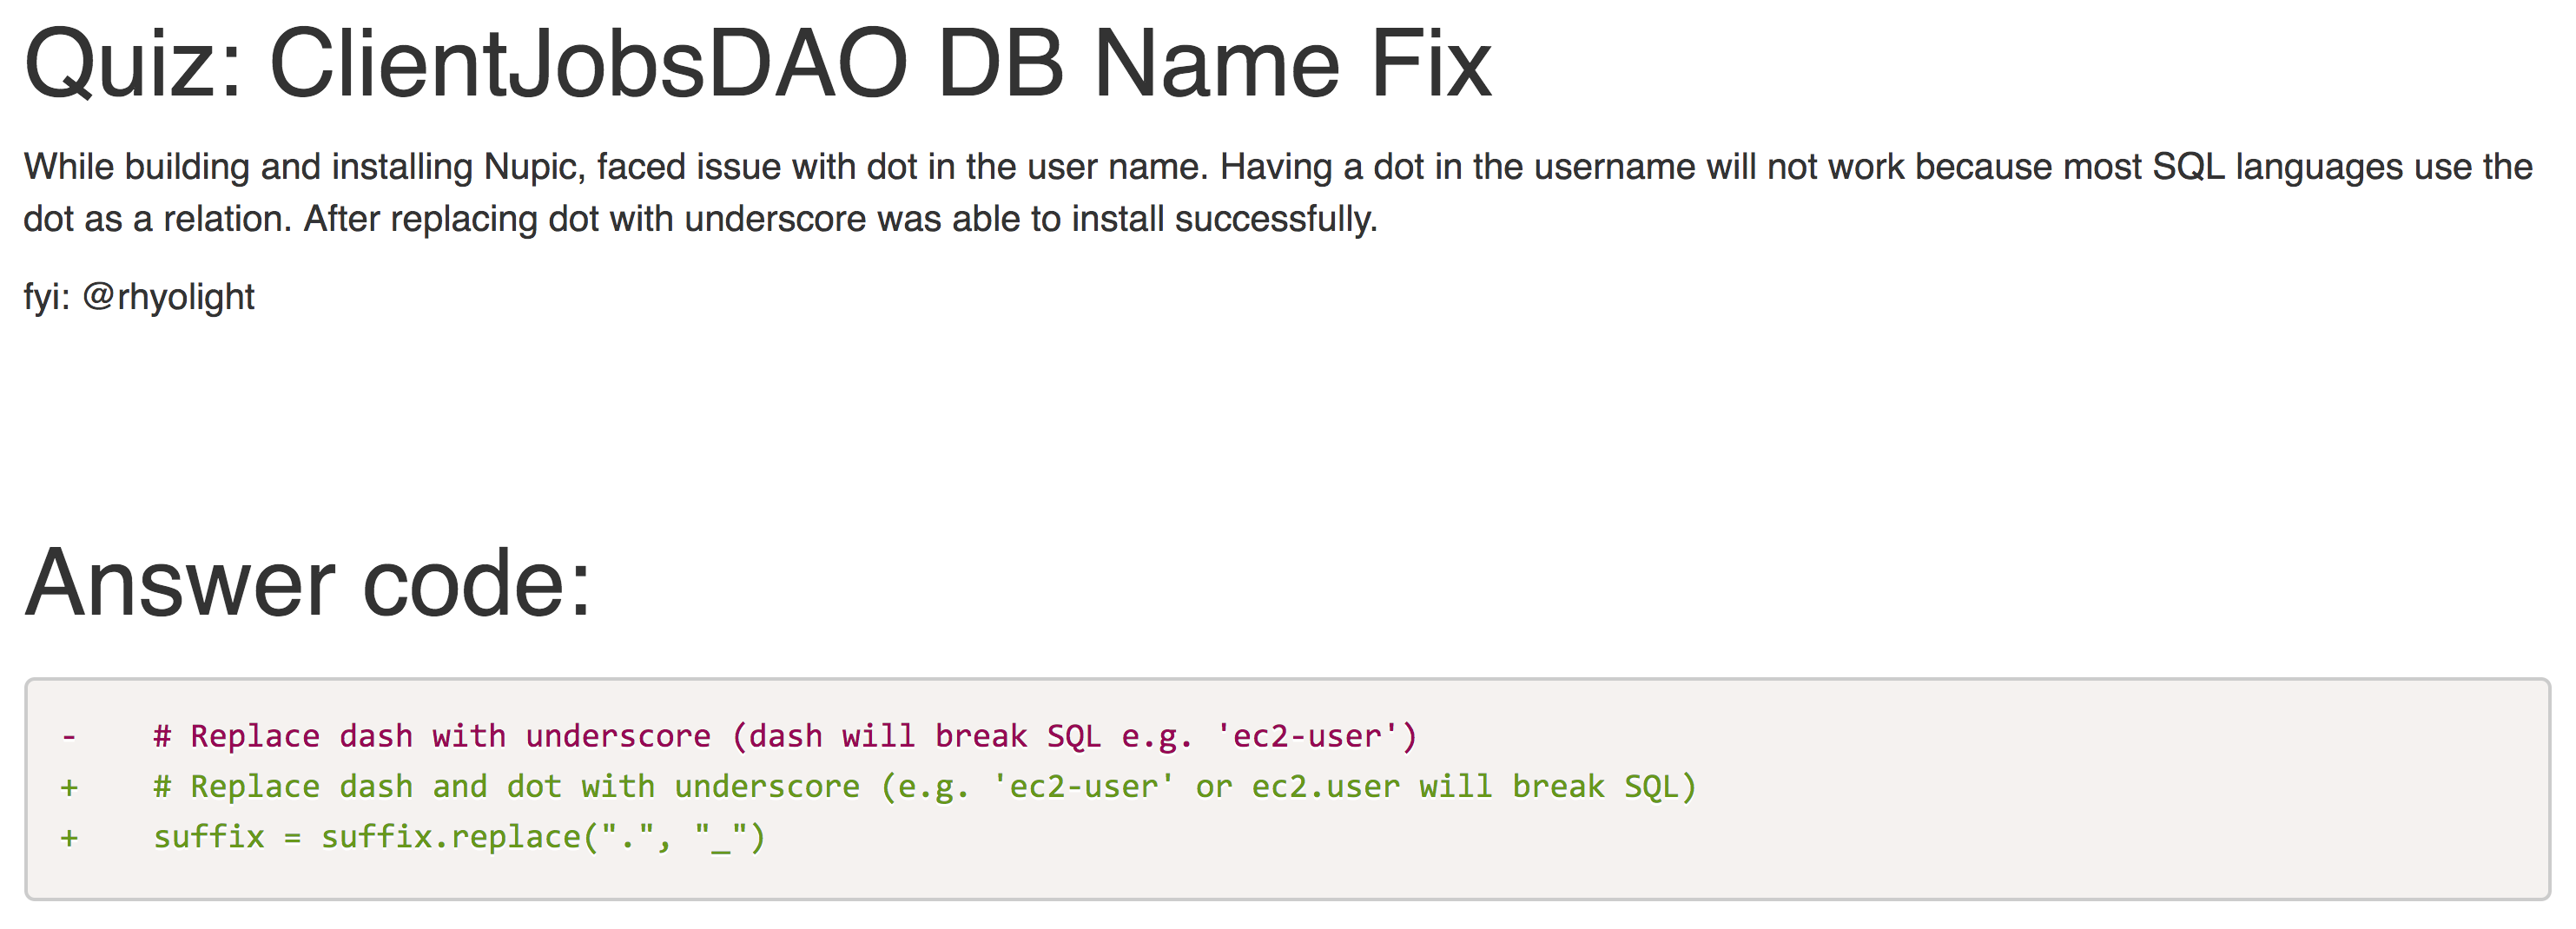
\includegraphics[width=0.95\columnwidth]{20190107-lab-study-experience-exercise.png}
  \caption{自分が経験した・見たことのあるバグの解決方法に関する演習問題の例.}
  \label{fig:lab-study-eg-experience}
  \vspace{-0.2cm}
\end{figure}


\subsection{ライブラリやAPIの使い方に関する演習問題}

実際のソフトウェア開発では,既に機能がパッケージとして実装されたライブラリを活用することで開発を効率的に進めている~\cite{Leveraging_API}.
図\ref{fig:lab-study-eg-lib}に示す演習問題の例は,Pythonのseaborn\footnote{\url{https://github.com/mwaskom/seaborn}}というデータの可視化に使用されるライブラリにおける,表のグリッド線の表示方法に関する問題である.
このように,RealCodeの演習問題を通じてライブラリを使用する上で発生しうる問題を学習できる可能性がある.

\begin{figure}[H]
\vspace{0.3cm}
	\centering
  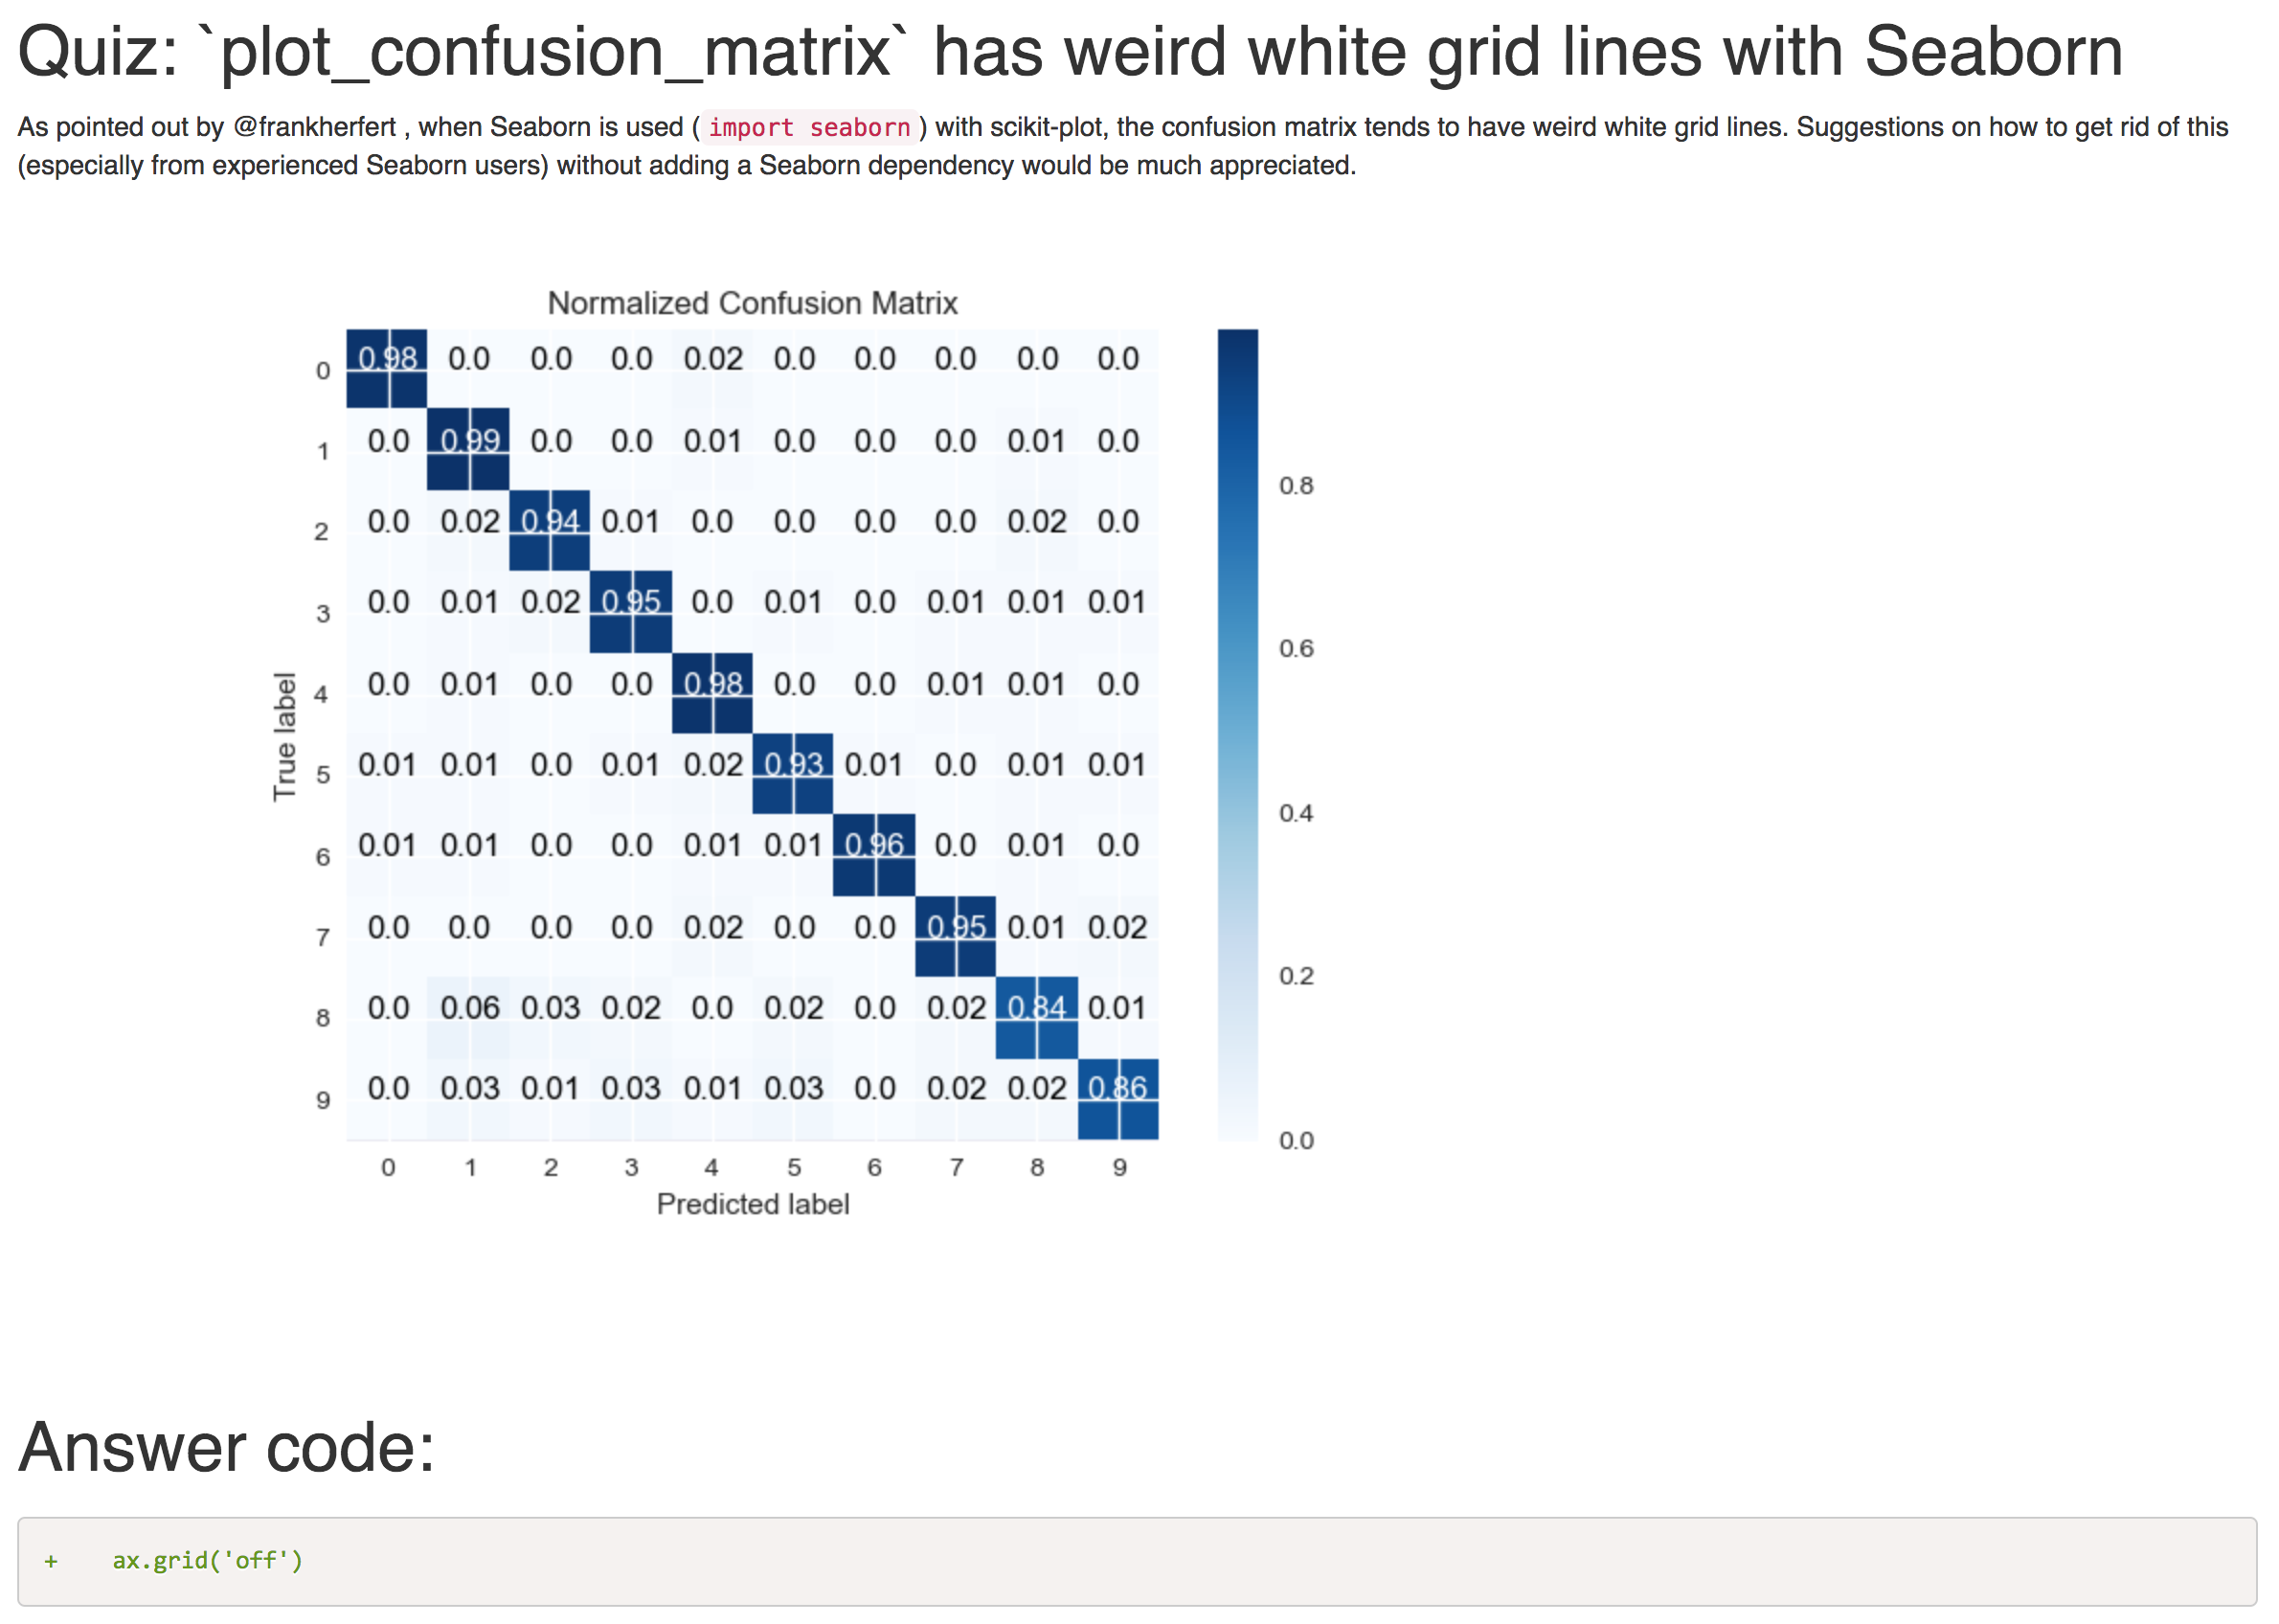
\includegraphics[width=1.0\columnwidth]{20190107-lab-study-lib-exercise.png}
  \caption{ライブラリやAPIの使い方に関する演習問題の例.}
  \label{fig:lab-study-eg-lib}
\end{figure}


%!TEX root = ../thesis.tex
%*******************************************************************************
%****************************** 7th Chapter **********************************
%*******************************************************************************
\chapter{考察}
\graphicspath{{Chapter7/Figs/}}

% Discussion

GitHubの膨大なイシューのデータから,プログラミング演習問題への転用に適さないイシューを分類するために,我々はヒューリスティックにより事前処理と決定木によるイシューの分類を行った.
決定木の精度を評価した結果,F値の平均が0.79の精度で転用に適さないイシューを取り除くことができた.
また,決定木による分類においては,変更行数が重要な特徴量であることが明らかとなった.
今後,イシューの説明文やコード変更内容に関する特徴量を新たに用いることで,より精度の高い分類器を実装できる可能性がある.

% Our quantitative examinations found a decision tree to select GitHub issues and code diff appropriate to repurpose to programming exercises.
% In particular, the numbers of lines in code diffs is the primary feature for classification.
% But the other features seemingly offered small contributions to the classification.
% Our work encourages future investigations on additional features in issue descriptions and code diffs as well as use of advanced machine learning methods.

% Sophisticated code syntax and semantic analysis could also contribute to selection accuracy.
% However, our investigation shows that a na\"{i}ve application of syntax analysis (i.e., whether a code diff causes a syntax error or not) does not perform well.
% Research may need an approach that exploits information in both issue descriptions and code diffs to identify valid exercises.
% This is a unique problem in a system like RealCode, and our work encourages future work to further investigate.

RealCodeが出題する演習問題の独自性評価から,GitHubのイシューを演習問題に転用する事で実現されたRealCodeの特徴が明らかとなった.
特に「本番環境におけるバグの影響を実感できる」という項目は実験参加者から多くの同意を得られた.
既存の学習環境とは異なり,本番環境ではソースコード中のバグがシステム障害やビジネスへの影響に直結する.
RealCodeの演習問題では,バグが引き起こす影響の大きさを体感することができ,これは実際のイシューを演習問題に転用する事で提供可能となった学習内容である.
% 一方でQ1(授業や教科書の問題と異なるか)に対し「同意しない」と判断された演習問題の多くが,プログラミング学習のために作られたリポジトリのイシューから出題されていた.
% 例えばPython-Guide-for-Beginners\footnote{\url{https://github.com/HarendraSingh22/Python-Guide-for-Beginners}}では,Python初学者を対象としたサンプルのプログラムを多く掲載しており,簡単な演算を実装する演習問題をイシューの形式で提供している.
% このようなリポジトリでは本研究が対象とするソフトウェア開発は行われていないので,RealCodeのデータセットから除外する仕組みが必要であると考える.





8人の学生に対するRealCodeに関するインタビューにおいて,実験参加者らはRealCodeが出題する演習問題が実践的であると指摘した.
特に授業で扱われているプログラミングと実際のソフトウェア開発の違いがインタビューから明らかとなった.
RealCodeの演習問題のさらなる検証が必要ではあるものの,RealCodeが出題する演習問題では既存の学習環境にはない内容を提供可能である事が分かった.

% The informal qualitative study uncovered participants' agreement on perceived uniqueness RealCode exercises demonstrate.
% They appreciated connections with real-world development, and it is exactly the outcome this work aims at.
% Although future work needs further validations, we show a strong potential of RealCode in capabilities to offer programming exercises that are not commonly available in existing learning materials.


一方,本研究にはさらなる検証や改良を要する点が存在する.
本研究の目的はGitHubのイシューをプログラミング演習問題に転用する事の実現可能性を検証することであるため,RealCodeが出題する演習問題の学習効果の評価を行っていない.
また,現在のRealCodeのプロトタイプは,選択されたプログラミング言語に該当する演習問題をランダムに提供している.
例えば難易度や内容に応じて演習問題を出題されるようになれば,ユーザのより体系的な学習を支援できるだろう.
そのためには,イシューの説明文やコード変更内容を解析し,演習問題の難易度や内容を推定する仕組みを調査する必要があると考える.

また,RealCodeが出題する演習問題の独自性評価では,Q1(授業や教科書の内容と異なるか)に対し36.44\%の演習問題が「同意しない」と判断された.
これらの演習問題を分析した結果,多くがプログラミング学習のために作られたリポジトリのイシューから出題されていた.
例えばPython-Guide-for-Beginners\footnote{\url{https://github.com/HarendraSingh22/Python-Guide-for-Beginners}}では,Python初学者を対象としたサンプルのプログラムを多く掲載しており,簡単な演算を実装する演習問題をイシューの形式で提供している.
このようなリポジトリでは本研究が対象とするソフトウェア開発は行われていないので,RealCodeのデータセットから除外する仕組みが必要であると考える.

学生に対するRealCodeのインタビュー評価では,3人の実験参加者ら(PC4,PC6,PC7)が,RealCodeの演習問題の背景を理解することが難しいと指摘した.
例えばPC6は,「前提知識が少し多い気がする,何を聞かれているのかが分かるまでに時間がかかる」と述べた.
イシューやプルリクエストの説明文だけでなく,リポジトリの説明文やファイル構造なども提供することで,演習問題の解答に必要な情報を補足することができると考える.


% This work has several limitations to be noted.
% It does not examine the learning effect of RealCode as our main scope is to uncover the feasibility of repurposing GitHub issues and code diffs to programming exercises.
% The current RealCode prototype na\"{i}vely chooses an exercise at random.
% This does not necessarily support strategic learning, such as starting with easy problems and moving to more advanced, or concentrating on a particular topic.
% Future work may study how useful issue descriptions in addition to code diffs could be to determine the difficulty and scope of a given exercise.

% Our issue screening and selection heuristics resulted in 4,722 issues, and are sufficient for the RealCode prototype.
% Exercises using these issues cover 61 different programming, markup, and configuration languages.
% RealCode thus can support learning of minor languages and experiencing infrequent development activities.


% % Limitation
% Although our informal qualitative study revealed a strong potential of RealCode, currently there are several limitation in the system.
% Most existing programming exercises clearly define what learners can study from them (e.g., exercises to learn List).
% However, the current RealCode prototype randomly provide exercises of a given programming language.
% Future work should investigate categorization of exercises by not only code content (e.g., list and method) but also development content (e.g., network and database).

% Our tool extracts only issues that satisfy our issue screening and selection heuristics.
% However, still there are other appropriate issues and pull requests on GitHub for programming learning.
% Exploring another approach of issue extraction for exercise use is important for future work.




%!TEX root = ../thesis.tex
%*******************************************************************************
%****************************** Eighth Chapter *********************************
%*******************************************************************************
\chapter{おわりに}
\graphicspath{{Chapter8/Figs/}}


本論文では,GitHubのイシューをプログラミング演習問題へと転用するシステムであるRealCodeについて述べた.
TA経験者および学生によるシステム評価を通して,イシューをプログラミング演習問題へと転用することで,既存の学習環境にはない独自の演習問題を提供可能であることが明らかとなった.

今後の課題として,考察で述べたシステムのさらなる改良,および学習効果の評価のほか,演習問題を提供するインタフェースの改良が挙げられる.
例えば,よりインタラクティブ性のあるもの(例えば,解答に時間がかかっている場合にはヒントを与えるなど)などを取り入れることが考えられる.
また,スマートフォンなどのモバイルデバイス上で学習できるようにすることで,学習者のすきま時間を利用した学習を支援するなど,新しい形のプログラミング学習を実現できると考える.
本研究で得られた知見をもとにして,プログラミング演習問題システムがさらに発展していくことを期待する.

% ********************************** Back Matter *******************************
% Backmatter should be commented out, if you are using appendices after References
%\backmatter

% ********************************** Bibliography ******************************
\begin{spacing}{0.9}

% To use the conventional natbib style referencing
% Bibliography style previews: http://nodonn.tipido.net/bibstyle.php
% Reference styles: http://sites.stat.psu.edu/~surajit/present/bib.htm

%%発表文献------------------------------------------------
\chapter*{Publications}
\addcontentsline{toc}{chapter}{Publications}

\section*{本研究に関する発表}
% \subsection*{国内研究会}
\begin{itemize}
\item \underline{柴藤大介},矢谷浩司.「GitHubのプルリクエストを用いたプログラミング課題自動生成システムの実現可能性に関する検討」第80回情報処理学会全国大会,2018年3月.\textbf{学生奨励賞受賞}.
\item \underline{柴藤大介},三島潤平,矢谷浩司.「GitHubのプルリクエストを用いた プログラミング課題自動生成システム」第4回SIGPX勉強会,2018年3月.
\end{itemize}

\section*{その他の発表}
\begin{itemize}
\item\underline{下尾波輝}, 矢谷浩司, KnowledgeDeck: ビジネス資料作成向け情報収集・整理支援システム,情報処理学会 第80回全国大会(発表予定).
\end{itemize}
% \renewcommand{\bibname}{Publications}
% \begin{thebibliography}{9}
%     \bibitem{hashizume_ubi} 橋爪崇弘, 矢谷浩司, 指尖容積脈波を同時に取得する指紋認証システムの試作と評価, 第53回情報処理学会UBI研究会, Vol.2017-UBI-53, No.56, March 2017.
%     \bibitem{hashizume_imwut} Takahiro Hashizume, Takuya Arizono, Koji Yatani, ``Auth `n' Scan: Opportunistic Photoplethysmography in Mobile Fingerprint Authentication,'' Proceedings of the ACM on Interactive, Mobile, Wearable and Ubiquitous Technologies (IMWUT), vol.1, No.4, Article \xxx, December 2017.
% \end{thebibliography}
%%------------------------------------------------------

\renewcommand{\bibname}{References}
\bibliographystyle{References/ACM-Reference-Format}
\cleardoublepage
\bibliography{References/master} % Path to your References.bib file


% If you would like to use BibLaTeX for your references, pass `custombib' as
% an option in the document class. The location of 'reference.bib' should be
% specified in the preamble.tex file in the custombib section.
% Comment out the lines related to natbib above and uncomment the following line.

%\printbibliography[heading=bibintoc, title={References}]

\end{spacing}

% ********************************** Appendices ********************************

% \begin{appendices} % Using appendices environment for more functunality

% \include{Appendix1/appendix1}
% \include{Appendix2/appendix2}

% \end{appendices}

% *************************************** Index ********************************
% \printthesisindex % If index is present

\end{document}